%Compiling with XeLaTeX
\documentclass[twoside,
			   openright, %chapter starts on the right, take care of the manually placed cleardoublepage commands
			   parskip=half, %1.5 line distance
			   11pt]{scrreprt}

%Presettings			   
%Personel Data
\title{Spectral Functions of Ultracold Fermi Gases \\ from Dyson-Schwinger Equations}
\author{Eugen Dizer}
\date{\today}

%Statements
\newtheorem{statements}{Statements}[chapter]


%Page Layout and Geometry
\usepackage{fancyhdr}
\fancyhfoffset{0pt}

\usepackage[a4paper,
			width = 150mm,
			top = 30mm,
		    bottom=30mm,
		    bindingoffset = 7mm
		    ]{geometry}

\usepackage{nicefrac}


%Chapter Layout (simple delete for standard appearance)
\KOMAoption{chapterprefix}{true}
\renewcommand*\raggedchapter{\centering}
\RedeclareSectionCommand[beforeskip=0pt,afterskip=2\baselineskip]{chapter}
\setkomafont{chapterprefix}{\Large\normalfont}
\addtokomafont{disposition}{\rmfamily}
\renewcommand*{\chapterformat}{%
  \chapappifchapterprefix{\nobreakspace}\thechapter%
  \IfUsePrefixLine{%
    \par\nobreak\vspace{-\parskip}\vspace{-.6\baselineskip}%
    \rule{0.9\textwidth}{0pt}\vspace{-1\baselineskip}%
  }{\enskip}%
}

%Quotes
\makeatletter
\newenvironment{chapquote}[2][2em]
  {\setlength{\@tempdima}{#1}%
   \def\chapquote@author{#2}%
   \parshape 1 \@tempdima \dimexpr\textwidth-2\@tempdima\relax%
   \itshape}
  {\par\normalfont\hfill--\ \chapquote@author\hspace*{\@tempdima}\par\bigskip}
\makeatother

%Bold Math in Titles
\makeatletter
\DeclareRobustCommand*{\bfseries}{%
   \not@math@alphabet\bfseries\mathbf
   \fontseries\bfdefault\selectfont
   \boldmath
}
\makeatother


%Page Layout For Beginning Of Chapter
\fancypagestyle{plain}{%
	\fancyhf{}  %clear all header and footer fields
	\fancyfoot[C]{\bfseries{\thepage}}
	\renewcommand{\headrulewidth}{0pt}
	\renewcommand{\footrulewidth}{0pt}
	}

%Page Layout For Other Pages
\pagestyle{fancy}
\renewcommand{\sectionmark}[1]{\markright{\thesection ~ \ #1}}
\renewcommand{\chaptermark}[1]{\markboth{ \chaptername\ \thechapter ~ \ #1}{}}
	\fancyhf{}
	\fancyhead[LE]{\bfseries{\thepage}\ ~ \normalfont\leftmark}
	\fancyhead[RO]{\rightmark\ ~ \bfseries{\thepage}} 	
	\renewcommand{\headrulewidth}{0pt}
	\renewcommand{\footrulewidth}{0pt}
	
	
%Headings
\setkomafont{section}{\textsf\bfseries\Large}
\setkomafont{subsection}{\textsf\bfseries\large}
\setkomafont{subsubsection}{\textsf\bfseries\normalsize}


%Maths and Units
\usepackage{amsmath, amsthm, amssymb, commath, mathtools, bm} %amsthm conflicts with ntheorem
\usepackage{revsymb}
\usepackage{slashed}
%\usepackage[hyperref]{ntheorem}
\usepackage{xfrac}


%Tikz and Plots
\usepackage{tikz}
\usepackage{pgf}


\usepackage{calc}

%Tables
\usepackage{array} %math mode in tables
\usepackage{booktabs} %hline rules

%Language Settings and Microtype
\usepackage{fontspec, xunicode}
%\usepackage[utf8]{inputenc}
%\usepackage{lmodern}
\usepackage{microtype}

\usepackage[ngerman,english]{babel}
\usepackage{csquotes}

%Useful Packages
\usepackage{graphicx} %including images
\usepackage{pdfpages} %including pdfs
\usepackage{float} %better positioning for float environments
\usepackage{blindtext} %for testing the output
\usepackage[labelfont=bf]{caption} %nice captions
\usepackage{subfigure} %for multiple plots


%Appendix and Bibliography
\usepackage[toc,page]{appendix}

\usepackage{etoolbox}
\appto\appendix{\addtocontents{toc}{\protect\setcounter{tocdepth}{0}}}

%reinstate the correct level for list of tables and figures
\appto\listoffigures{\addtocontents{lof}{\protect\setcounter{tocdepth}{1}}}
\appto\listoftables{\addtocontents{lot}{\protect\setcounter{tocdepth}{1}}}

\usepackage[backend=biber]{biblatex}
\bibstyle{bib/utphys.bst}
\addbibresource{bib/msc.bib}

%Colorlinks etc.
\usepackage[colorlinks=True]{hyperref}
\hypersetup{allcolors=BScBlue}
%Statement environment
\newcommand{\statement}[1]{\stepcounter{statements}\begin{center}
	\textbf{#1}
	\end{center}
}

%Color Settings
\usepackage{xcolor}
\definecolor{BScRed}{RGB}{157,0,0}
\definecolor{BScBlue}{RGB}{1,1,141}


%Useful definitions
\newcommand{\rstate}[1]{\left\vert #1 \right\rangle}
\newcommand{\lstate}[1]{\left\langle #1 \right\vert}
\newcommand{\expectation}[1]{\left\langle #1 \right\rangle}
\newcommand{\vacuum}[1]{\langle 0 \vert #1 \vert 0 \rangle}
\newcommand{\xint}[1]{\int d^3x \ #1}
\newcommand{\pint}[1]{\int \frac{d^4p}{(2\pi)^4} \ #1 \ e^{-i p (x-x')}}





\begin{document}

\pagenumbering{roman}
%Introductory stuff, abstracts and toc
{\hypersetup{allcolors=black}
\begin{titlepage}

	\begin{center}
		\makeatletter
		\vspace{2cm}
		\Large\textbf{Department of Physics and Astronomy\\
			Heidelberg University}
		
		%\vspace{13cm}
		\vfill
		\normalsize
		Master Thesis in Physics\\
		\normalsize
		submitted by\\[0.4cm]
		\Large
		\textbf{\href{mailto:eugen9898@web.de}{\@author}}\\[0.4cm]
		\normalsize
		born in Omsk (Russia)\\[0.4cm]
		\Large
		\textbf{2023}
		
        \thispagestyle{empty}
		\cleardoublepage
		\thispagestyle{empty}
		\LARGE\textbf{\@title}\\[.4cm]

		\vfill
		\normalsize
		This Master Thesis has been carried out by \\ 
		\vspace{3pt}
		\textbf{\href{mailto:eugen9898@web.de}{\@author}}  \\ 
		\vspace{3pt}
		at the\\
		\vspace{3pt}
		\textbf{Institute for Theoretical Physics in Heidelberg}\\
		\vspace{5pt}
		under the supervision of\\
		\vspace{5pt}
		\textbf{Prof. Dr. Jan M. Pawlowski} 
		
		\makeatother
	\end{center}
\cleardoublepage
\end{titlepage}
}
{\hypersetup{allcolors=black}
\thispagestyle{plain}

\makeatletter

\begin{center}
\textbf{\Large\@title} \\
\vspace{.1cm}
\@author \\
\end{center}

\makeatother

\vspace*{1cm}

%Abstract in english language
\statement{\large Abstract}
A single-channel model with Hubbard-Stratonovich field is used to study ultracold Fermi gases at finite temperature in the normal and superfluid phase. Non-perturbative real-time Green's functions with full frequency and momentum dependence are computed iteratively from Dyson-Schwinger equations. Employing the spectral representation, Matsubara sums are evaluated and analytically continued to real frequencies. In this way, the full spectral functions are calculated directly without the need of numerical reconstruction methods. Finally, these techniques are applied to the unitary Fermi gas and the Fermi polaron.

\vfill

%Abstract in german language
\begin{otherlanguage}{ngerman}
\statement{\large Zusammenfassung}
Ein Einkanal-Modell mit Hubbard-Stratonovich Feld wird verwendet, um ultrakalte Fermi\-gase bei endlicher Temperatur in der normalen und suprafluiden Phase zu untersuchen. Nicht-perturbative Realzeit-Greensfunktionen mit voller Frequenz- und Impulsabhängigkeit werden iterativ aus Dyson-Schwinger Gleichungen berechnet. Unter Verwendung der spektralen Darstellung werden Matsubarasummen ausgewertet und analytisch zu reellen Frequenzen fortgesetzt. Auf diese Weise werden die vollen Spektralfunktionen direkt berechnet, ohne auf numerische Rekonstruktionsmethoden angewiesen zu sein. Schließlich werden diese Techniken auf das unitäre Fermigas und das Fermi Polaron angewendet.
\end{otherlanguage}
\vfill
}
{\hypersetup{linkcolor=black}
\tableofcontents  
}
\cleardoublepage


\setcounter{tocdepth}{1}
\pagenumbering{arabic}

%Main part
	\chapter{Introduction}
\label{chapter:introduction}

\begin{chapquote}[2em]{Jan M. Pawlowski}
``There is no free lunch.''
\end{chapquote}

The experimental control of ultracold Fermi gases provides a powerful tool for studying strongly correlated quantum systems including the BCS-BEC crossover~\cite{Randeria2014} and Fermi polarons~\cite{Parish2023}. Understanding these exotic quantum phenomena is essential for the future development of high-temperature superconductors and quantum computers.

Various non-perturbative approaches, such as Quantum Monte Carlo (QMC) simulations \cite{Magierski2009,Prokofev2008}, selfconsistent T-matrix theory~\cite{Hanai2013,Pini2019} or the Luttinger-Ward formalism~\cite{Haussmann1999,Haussmann2007}, as well as Dyson-Schwinger equations (DSEs)~\cite{Boettcher2013,Diener2008} and functional Renormalization Group (fRG) methods~\cite{Diehl2006-2,Diehl2010} have been employed to describe strongly interacting fermions.

A central object of interest in real-time applications is the spectral function~\cite{Kallen1952,Lehmann1954} which encodes information about scattering properties and the energy spectrum of the system. Its determination requires knowledge of correlation functions at real frequencies. However, the approaches mentioned above are usually formulated in imaginary frequencies by construction or due to significantly reduced computational costs for the calculation of thermodynamic observables~\cite{Frank2018}. This leaves an ill-conditioned numerical problem when analytically continuing to real frequencies~\cite{Wink2020}.

Numerical reconstruction methods, such as Padé approximations~\cite{Schmidt2011} or the Maximum Entropy Method~\cite{Haussmann2009} have been utilized to obtain spectral functions from imaginary-time data. However, these techniques are plagued by large systematic uncertainties and cannot guarantee a correct result. Therefore, a direct real-time computation is favorable.

In this Thesis, functional methods are used to calculate spectral functions of ultracold Fermi gases directly in real frequencies without the need of numerical reconstruction methods. As a proof of principle, the selfconsistent real-time framework is applied to the well-known spin-balanced BCS-BEC crossover and the Fermi polaron problem. Previous results are verified and novel spectral functions are presented.

This work is organized as follows. In Chapter~\ref{chapter:functional-methods}, the functional description of Quantum Field Theories (QFTs) at finite temperature and the spectral representation of propagators are introduced briefly. In Chapter~\ref{chapter:ultracold-gases}, the theoretical background of ultracold Fermi gases is presented. In this context, the microscopic model of the theory and first mean-field considerations are discussed. The main part of this work is summarized in Chapter~\ref{chapter:bcs-bec-crossover} and deals with the spectral properties of the BCS-BEC crossover phase diagram, see Fig.~\ref{fig:crossover-phase-diagram}. In particular, the normal phase above the critical temperature is investigated in detail and a brief outlook towards the superfluid phase is given. Analytical and numerical results are discussed and compared to other works. In Chapter~\ref{chapter:fermi-polaron}, the selfconsistent functional approach is applied to the Fermi polaron problem and compared with previous works. Finally, in Chapter~\ref{chapter:conclusion}, important results are summarized and a small outlook for future work is given.


\begin{figure}[h]
\centering
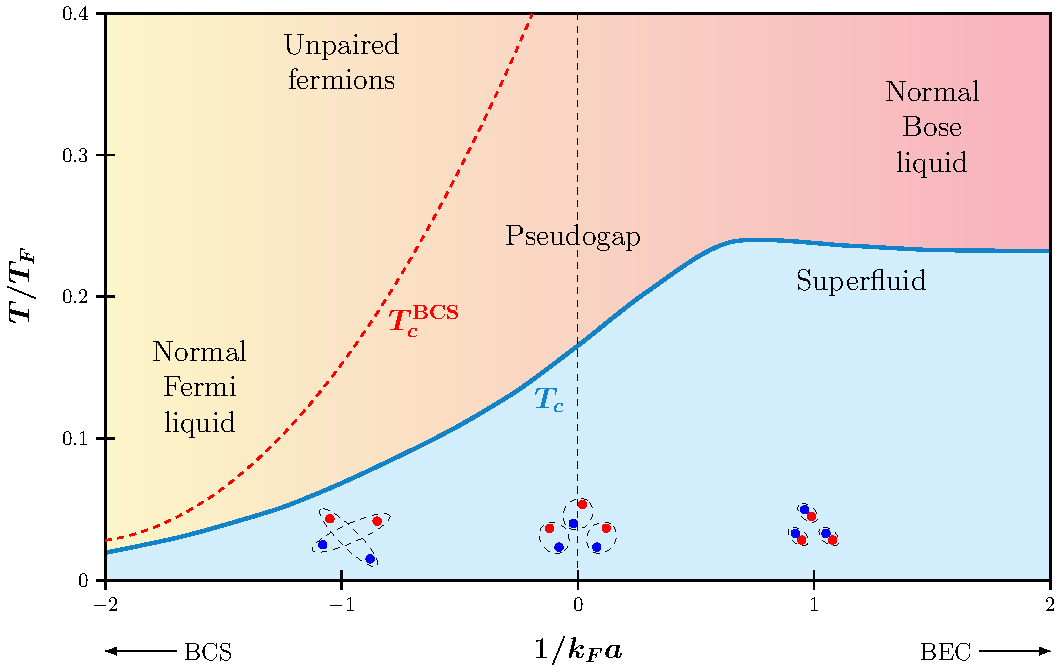
\includegraphics[width=0.75\linewidth]{figs/bcs-bec.pdf}
\caption[Phase diagram of the BCS-BEC crossover]{Phase diagram of the BCS-BEC crossover as a function of temperature $T/T_F$ and coupling strength $1/k_Fa$, where $T_F$ and $k_F$ is the Fermi temperature and momentum, respectively, and $a$ is the two-body scattering length. Inspired by~\cite{Randeria2014} with new results from~\cite{Haussmann2007}.}
\label{fig:crossover-phase-diagram}
\end{figure}


\section*{Notation and Units}

In this Thesis, natural units with $\hbar = c = k_B = 2m = 1$, where $m$ is the fermion mass, are used. All dimensionful quantities are measured in terms of the density $n$, or Fermi momentum $k_F=(3\pi^2n)^{1/3}$. Temperature and energy-like quantities are measured in terms of Fermi energy $T_F=\varepsilon_F=k_F^2$. Sometimes, dimensionful constants are reintroduced to remind the reader of the correct units. Three-vectors are denoted by bold letters. For the sake of simplicity, we use the same notation for the fields $\psi_{\sigma}$, with fermion species $\sigma=(\uparrow,\downarrow)$, and $\phi$ in the classical and effective action.

We use the integral conventions
\begin{align}
	\int_x = \int d^dx \quad \mathrm{and} \quad  \int_p = \int \frac{d^dp}{(2\pi)^d} \,.
\end{align}

	\chapter{Functional Methods}
\label{chapter:functional-methods}

In this Chapter, the basic theoretical tools of this work are introduced briefly. Functional methods, such as the DSEs or the fRG, provide non-perturbative relations for the full correlation functions of a quantum field theory. For more detailed reviews, see~\cite{Swanson2010} (DSEs) and~\cite{Kopietz2010,Pawlowski2007} (fRG). In the following, we will put emphasis on Dyson-Schwinger equations and field theories at finite temperature. At the end of this Chapter, we discuss the spectral representation.

\section{Dyson-Schwinger equations}
\label{section:dyson-schwinger-equations}

Functional methods are based on the path integral formulation of QFT. In general, a QFT is described by the microscopic action $S[\phi]$. Analogously to statistical physics, the generating functional $Z[J]$ can be written in Euclidean spacetime as
%
\begin{align}
	\label{eq:generating-functional}
	Z[J] = \frac{1}{\mathcal{N}} \int \mathcal{D}\phi\; \mathrm{e}^{-S[\phi]+J\cdot\phi} \quad \mathrm{with} \quad J\cdot\phi\equiv\int_x\;J(x)\phi(x)\,,
\end{align}
%
where $\mathcal{N}$ is a normalization constant, $J(x)$ is some external source field, and $\int\mathcal{D}\phi$ is the functional integral over all possible field configurations $\phi$. The correlation functions are then obtained by functional derivatives with respect to the source fields,
%
\begin{align}
	\label{eq:correlation-functions}
	\langle \phi(x_1)\dots\phi(x_n)\rangle = \frac{1}{Z[0]}\frac{\delta^n Z[J]}{\delta J(x_1)\dots\delta J(x_n)} \Bigg|_{J=0} \,.
\end{align} 
%
By the reconstruction theorem, a quantum field theory is completely determined by its correlation functions~\cite{Wightman1956}. Thus, the path integral contains the full information of the theory. 
However, it can be shown that the correlation functions in Eq.~\eqref{eq:correlation-functions} contain redundant information and can be split into a connected and disconnected part. In case of a two-point function~\cite{Peskin1995},
%
\begin{align}
	\label{eq:two-point-function}
	\langle \phi(x_1)\phi(x_2)\rangle = \langle \phi(x_1)\phi(x_2)\rangle_c + \langle\phi(x_1)\rangle\langle\phi(x_2)\rangle \,,
\end{align}
%
where $c$ denotes the connected part of the correlation function in which all external lines of the Feynman diagrams are connected. This redundancy is removed by the Schwinger functional $W[J]$, which generates only connected correlation functions,
%
\begin{align}
	\label{eq:schwinger-functional}
	W[J] = \ln Z[J] \,.
\end{align}
%
In particular, the full propagator is defined by the connected two-point function~\cite{Peskin1995},
%
\begin{align}
	\label{eq:propagator-schwinger}
	G(x_1,x_2) = \langle \phi(x_1)\phi(x_2)\rangle_c = \frac{\delta^2 W[J]}{\delta J(x_1)\delta J(x_2)} \Bigg|_{J=0} \,,
\end{align}
%
and can be obtained by Dyson resummation of amputated one-particle-irreducible (1PI) contributions. Here, 1PI refers to Feynman diagrams which cannot be divided into two separate diagrams by cutting one internal line. 

Thus, the entire information of the theory is already encoded in the 1PI diagrams. The generating functional of 1PI correlation functions is the quantum effective action $\Gamma[\Phi]$, which is defined as the Legendre transform of the Schwinger functional,
%
\begin{align}
	\label{eq:effective-action}
	\Gamma[\Phi] = \sup_J\big[J\cdot\Phi - W[J]\big] = J_{\sup}\cdot\Phi - W[J_{\sup}] \,,
\end{align}
%
where $\Phi=\langle\phi\rangle$ is now the mean field and $J_{\sup} = J_{\sup}[\Phi]$ is the field-dependent current that minimizes~\eqref{eq:effective-action}. From a physical point of view, the effective action $\Gamma$ is the quantum analogue of the classical action $S$, which accounts for all quantum corrections. A non-perturbative connection between the quantum and classical equations of motion is provided by the Dyson-Schwinger equation (DSE)~\cite{Dyson1949,Schwinger1951},
%
\begin{align}
	\label{eq:DSE}
	\frac{\delta\Gamma}{\delta\Phi}\left[\Phi\right] = \frac{\delta S}{\delta\phi}\left[\phi=\Phi+G\cdot\frac{\delta}{\delta\Phi}\right] \,,
\end{align}
%
which follows from the shift independence of the path integral measure. A more detailed derivation and discussion can be found in~\cite{Pawlowski2021}. The product in the argument of Eq.~\eqref{eq:DSE} is defined by
%
\begin{align}
	\label{eq:propgator-derivative}
	G\cdot\frac{\delta}{\delta\Phi} = \int_x G(x_1,x)\cdot\frac{\delta}{\delta\Phi(x)} \,.
\end{align}
%
All higher order 1PI correlation functions are obtained by functional derivatives with respect to the mean field $\Phi$,
%
\begin{align}
	\label{eq:1PI-correlation-functions}
	\Gamma^{(n)}(x_1,\dots,x_n)=\frac{\delta^n\Gamma[\Phi]}{\delta\Phi(x_1)\dots\delta\Phi(x_n)} \,.
\end{align}
%
It can be shown that the two-point function is exactly the inverse of the full propagator,
%
\begin{align}
	\label{eq:propagator-gamma}
	\Gamma^{(2)}(x_1,x_2) = G^{-1}(x_1,x_2) \,.
\end{align}
%
Note that this is a matrix equation in general. Thus, the inversion must account for all off-diagonal terms. In the following, we summarize the main extensions when dealing with multiple fields of different species.

For a general set of fermionic and bosonic fields, one can introduce a superfield $\Phi$ which collects all field indices and species. In case of ultracold Fermi gases, the superfield is given by $\Phi=(\psi_{\sigma},\psi_{\sigma}^*,\phi,\phi^*)$ with fermion species $\sigma=(\uparrow,\downarrow)$. The Dyson-Schwinger equation takes the form
%
\begin{align}
	\label{eq:DSE-general}
	\frac{\delta\Gamma}{\delta\Phi_a}\left[\Phi\right] = \frac{\delta S}{\delta\phi_a}\left[\phi_b=\Phi_b+G_{bc}\cdot\frac{\delta}{\delta\Phi_c}\right] \,,
\end{align}
%
where a sum over repeated indices is implied. Correlation functions are denoted by
%
\begin{align}
	\label{eq:super-correlation-functions}
	\Gamma^{(n)}_{\Phi_{a_1}\dots\Phi_{a_n}}=\frac{\delta}{\delta\Phi_{a_1}}\dots \frac{\delta}{\delta\Phi_{a_n}}\, \Gamma[\Phi] \,.
\end{align}
%
Finally, derivatives of propagators with respect to the mean fields are given by~\cite{Pawlowski2021}
%
\begin{align}
	\label{eq:derivative-propagator}
	\frac{\delta}{\delta\Phi_a} G_{bc} = -(-1)^{ab}(-1)^{ee} \, G_{bd}\cdot\Gamma^{(3)}_{dae}\cdot G_{ec} \,,
\end{align}
%
where $(-1)^{ab}=-1$, if $a$ and $b$ are fermionic, and $(-1)^{ab}=1$ otherwise. The relation between propagator and two-point function becomes $G_{ac}\cdot\Gamma^{(2)}_{cb}=(-1)^{ab}\delta_{ab}$.

This summarizes all necessary identities to work with functional methods in arbitrary theories involving fermions and bosons.

\section{Finite temperature and density}
\label{section:finite-temperature-density}

For a quantum field theory in thermal equilibrium, finite temperature can be introduced in analogy to classical statistical physics via the so called Matsubara formalism. More general approaches using e.g. Schwingers closed time path can be found in~\cite{LeBellac1996}. Here, we are mainly interested in the implications for the calculation of Feynman diagrams. 

In classical statistical physics, inverse temperature $\beta=1/T$ is the prefactor in front of the Hamiltonian in the partition function and can be viewed as a finite extent along imaginary times with $\tau=i\beta$. As a consequence, the imaginary time direction is compactified to the interval $\tau\in[0,\beta]$ and bosonic fields $\phi$ have to be periodic with period $\beta$, i.e.
%
\begin{align}
	\label{eq:periodic-condition}
	\phi(\tau+\beta,\bm{x})=\phi(\tau,\bm{x}) \,.
\end{align}
%
The finite temperature path integral can written as
%
\begin{align}
	\label{eq:finite-temperature-path-integral}
	Z = \int_{\phi(\beta,\bm{x})=\phi(0,\bm{x})} \mathcal{D}\phi\; \mathrm{e}^{-S[\phi]} \quad \mathrm{with} \quad S[\phi]=\int_0^{\beta}d\tau\int d^3x\, \mathcal{L}[\phi] \,,
\end{align}
%
where $\mathcal{L}$ is the imaginary-time (Euclidean) Lagrangian of the theory. The finite extent of the imaginary time axis and the periodic boundary condition have important consequences for the Fourier transform of fields,
%
\begin{align}
	\label{eq:matsubara-fourier-transform}
	\phi(\tau,\bm{x}) = T\sum_{\omega_n}\int\frac{d^3p}{(2\pi)^3}\, e^{-i(\tau\omega_n-\bm{x}\cdot\bm{p})}\, \phi(\omega_n,\bm{p})  \,,
\end{align}
%
where $\omega_n=2\pi n T$ with $n\in\mathbb{Z}$ are the so called Matsubara frequencies. Thus, the zero component of the momentum becomes discrete and the continuous integral turns into an infinite Matsubara sum, which can be evaluated using the residue theorem from complex analysis. To summarize, for the transformation of a QFT in vacuum to a QFT at finite temperature, one needs to perform the following replacement in appearing momentum integrals
%
\begin{align}
	\label{eq:finite-temperature-integrals}
	\int\frac{d^dp}{(2\pi)^d} \rightarrow T\sum_{\omega_n}\int\frac{d^{d-1}p}{(2\pi)^{d-1}}  \,.
\end{align}
%
In case of fermionic fields $\psi$, the path integral has to fulfill anti-periodic instead of periodic boundary conditions, i.e. $\psi(\tau+\beta,\bm{x})=-\psi(\tau,\bm{x})$. The Matsubara frequencies are given by $\omega_n=(2n+1)\pi T$ with $n\in\mathbb{Z}$.

The inclusion of a finite chemical potential $\mu$ leads to a finite density and follows also from the path integral in analogy to the grand canonical ensemble. Recall that the particle number is related to the chemical potential via derivative of the grand potential with respect to $\mu$. In order to include a chemical potential in the path integral, we add the respective term to the Euclidean action. In frequency space, this amounts to the following shift into the complex plane
%
\begin{align}
	\label{eq:chemical-potential}
	\omega_n \rightarrow \omega_n - i\mu \,.
\end{align}
%
Note that finite temperatures or densities break Lorentz and Galilei invariance in general, since they single out a specific frame of reference.

\section{Spectral representation}
\label{section:spectral-representation}

The spectral representation of the propagator plays a central role in the spectral functional approach. Usually, computations are performed in imaginary-time on discrete Matsubara frequencies $\omega_n$ which results in an ill-defined problem when analytically continuing to the real frequency axis, see Fig.~\ref{fig:spectral-properties}. In the present work, we assume the following Källén-Lehmann representation of the full propagators~\cite{Abrikosov1975,Fetter1971,Haussmann2009}
%
\begin{align}
	\label{eq:spectral-representation}
	G(\omega_n,\bm{p}) = \int_{-\infty}^{\infty} d\lambda \, \frac{\rho(\lambda,\bm{p})}{-i\omega_n+\lambda} \,,
\end{align}
%
where $\rho$ is the spectral function. In this way, the propagator is a symbolic expression in $\omega_n$ which can be evaluated at arbitrary frequencies in the complex plane. Physically, the spectral function acts as a linear response function of the propagator, encoding the energy spectrum of the theory, see also Fig.~\ref{fig:spectral-properties}. Eq.~\eqref{eq:spectral-representation} leads to the following inverse relation between the spectral function and the retarded propagator,
%
\begin{align}
	\label{eq:spectral-relation}
	\rho(\omega,\bm{p}) = \frac{1}{\pi}\, \mathrm{Im}\, G^R(\omega,\bm{p}) \,,
\end{align}
%
where $G^R(\omega,\bm{p})=G(-i(\omega+i0^+),\bm{p})$ and $\omega$ is now a real frequency. The existence of a spectral representation restricts all
non-analyticities of the propagator to lie on the real
frequency axis. For a more detailed discussion on the analytic properties, see~\cite{Perali2002,Rohe2001,Wink2020}. The fermionic spectral function satisfies the sum rule~\cite{Fratini2013}
%
\begin{align}
	\label{eq:spectral-sum-rule}
	\int_{-\infty}^{\infty} d\lambda\,\rho_{\psi}(\lambda,\bm{p}) = 1 \,.
\end{align}
%
However, while fermionic spectral functions satisfy $\rho_{\psi}(\omega,\bm{p}) \geq 0$, bosonic spectral functions satisfy $\mathrm{sgn}(\omega) \rho_{\phi}(\omega,\bm{p}) \geq 0$~\cite{Fetter1971}.
Note that the negative sign of the boson spectral function for negative frequencies guarantees the positivity of the boson momentum distribution function.
Moreover, the boson spectral function has not to be normalized.

\begin{figure}[b]
	\centering
	\subfigure[]{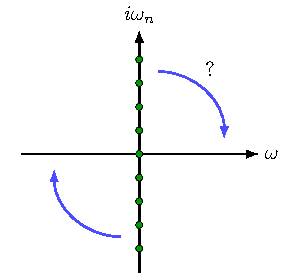
\includegraphics[width=0.3\textwidth]{figs/wick.pdf}} 
	\subfigure[]{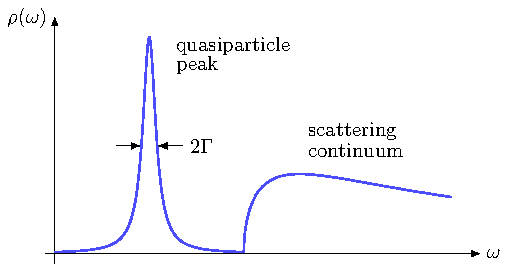
\includegraphics[width=0.55\textwidth]{figs/spectral.pdf}}
	\caption[Analytic continuation and spectral function]{(a) The problem of analytic continuation from discrete imaginary Matsubara frequencies $\omega_n$ to real frequencies $\omega$. (b) Sample spectral function $\rho(\omega,\bm{p}=0)$ featuring a broadened mass peak and a scattering continuum.}
	\label{fig:spectral-properties}
\end{figure}
	\chapter{Ultracold Fermi Gases}
\label{chapter:ultracold-gases}

In this Chapter, a short introduction to the physics of ultracold Fermi gases is given. First, the concept of Feshbach resonances, which allow to tune the interaction strength inside the gas, and their connection to scattering physics is introduced. Then, the microscopic model and first mean-field descriptions are discussed. For more details, see~\cite{Boettcher2012,Randeria2014,Zwerger2016}.

\section{Feshbach resonances}
\label{section:feshbach-resonances}

In ultracold fermionic gases, the interaction strength can be tuned by means of Feshbach resonances. In order to understand this statement, we have to recover the basic notion of two-body scattering physics at low energies. The relevant parameter, which can be extracted from experiments, is the scattering length $a$. For sufficiently short range interaction potentials, the scattering length describes the scattering process completely. At low temperatures, the s-wave scattering amplitude is given by~\cite{Zwerger2016}
%
\begin{align}
	\label{eq:scattering-amplitude}
	f(k) = \frac{1}{-1/a-ik+\mathcal{O}(k^2)} \,,
\end{align}
%
where $k$ is the center of mass momentum. In real gases, the effective range of interactions is essentially the van der Waals length $l_{\mathrm{vdw}}$ which is much smaller then the average interparticle spacing $n^{-1/3}$ at density $n$. At the same time, the temperature has to be small enough such that the thermal wavelength $\lambda_T$ is larger than the interparticle spacing. Ultracold gases are thus characterized by the following hierarchy of length scales~\cite{Zwerger2016}
%
\begin{align}
	\label{eq:hierarchy-of-scales}
	l_{\mathrm{vdw}} \ll n^{-1/3} \ll \lambda_T \,.
\end{align}
%
The difference between weak and strong interactions is characterized by the relative magnitude of the scattering length with respect to the interparticle distance. Using Feshbach resonances, the scattering length can be tuned to values much larger then the typical interparticle distance while keeping the effective range of order $l_{\mathrm{vdw}}$. In this way, strongly interacting Fermi gases with $n^{-1/3}a\gg 1$ can be realized.

In general, Feshbach resonances can be described with the two-channel model, see Fig.~\ref{fig:feshbach-resonances}. When a bound state in a closed channel is coupled resonantly with the scattering continuum of an open channel, the scattering cross section can be enhanced. Here, one uses the fact that the atoms can virtually change their spin configuration during the collision. In the different spin configuration, they interact with a different scattering potential which can be tuned with a magnetic field $B$ according to the Zeeman splitting $\Delta E=\Delta\mu B$, where $\Delta\mu$ is the difference in magnetic moment between closed and open channel. The energetic distance of the bound state in the closed channel to the scattering threshold $E=0$ is called detuning~\cite{Faigle-Cedzich2022}
%
\begin{align}
	\label{eq:detuning}
	\nu(B) = \Delta\mu (B-B_0) \,,
\end{align}
%
where $B_0$ is the resonance position of the Feshbach resonance, see Fig.~\ref{fig:feshbach-resonances}.

On a phenomenological level, the scattering length can be written as
%
\begin{align}
	\label{eq:scattering-length}
	a(B) = a_{\mathrm{bg}} \left(1-\frac{\Delta B}{B-B_0}\right) \,,
\end{align}
%
where $a_{\mathrm{bg}}$ is a background scattering length without coupling to the closed channel and $\Delta B$ is the width of the resonance. For more discussions about the width $\Delta B$, as well as broad and narrow Feshbach resonances, see e.g.~\cite{Diehl2006-1}. Note that the resonance occurs when the detuning vanishes $\nu(B)\rightarrow 0$. In this case, we are in the so called strongly correlated, unitary regime. To summarize, the following three regimes can be identified in the three-dimensional BCS-BEC crossover, as function of the dimensionless interaction strength $(k_Fa)^{-1}$,
%
\begin{align*}
	(k_F a)^{-1} \rightarrow -\infty \,&: \qquad \text{weakly interacting fermionic gas ,} \\
	|(k_F a)^{-1}| \leq 1 \,&: \qquad \text{strongly interacting regime ,} \\
	(k_F a)^{-1} \rightarrow \infty \,&: \qquad \text{weakly interacting bosonic gas .}
\end{align*}
%
In the following, we are interested in the strongly correlated case close to a broad Feshbach resonance which is described sufficiently by the single-channel model introduced below.


\begin{figure}[t]
	\centering
	\subfigure[]{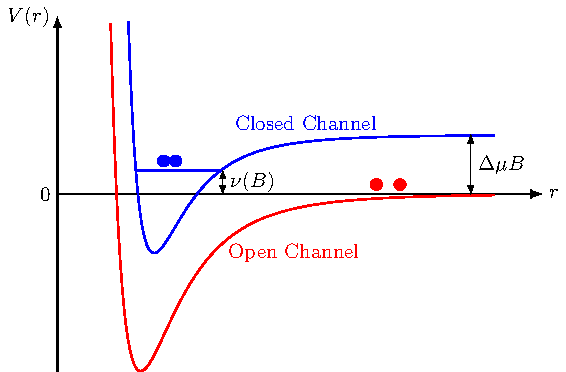
\includegraphics[width=0.49\textwidth]{figs/feshbach.pdf}} 
	\subfigure[]{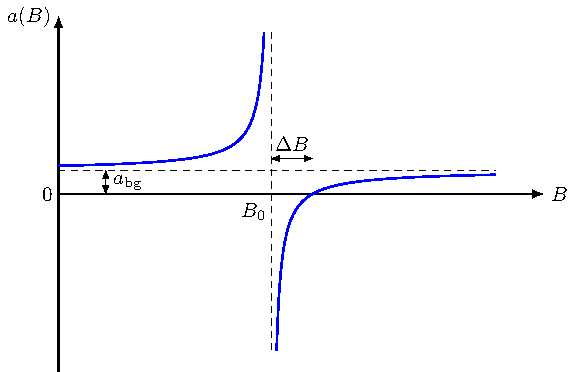
\includegraphics[width=0.49\textwidth]{figs/scattering.pdf}}
	\caption[Feshbach resonance model and scattering length]{(a) Two-channel Feshbach resonance model as described in the main text. (b) Scattering length $a$ as a function of magnetic field $B$, see Eq.~\eqref{eq:scattering-length}.}
	\label{fig:feshbach-resonances}
\end{figure}


\section{Single-channel model}
\label{section:single-channel-model}

We consider a non-relativistic two-component Fermi gas with contact interaction described by the Euclidean action (single-channel model)~\cite{Zwerger2016}
%
\begin{align}
	\label{eq:microscopic-action}
	S[\psi] = \int_{0}^{\beta} d\tau \int d^3 x\,
	\Big[ \sum_{\sigma=\uparrow,\downarrow} \psi_{\sigma}^* (\partial_{\tau} - \nabla^2 - \mu_{\sigma}) \psi_{\sigma}
	+ \lambda \psi_{\uparrow}^*\psi_{\downarrow}^*\psi_{\downarrow}\psi_{\uparrow} \Big] \,,
\end{align}
%
where $\lambda$ is the coupling constant, which is connected to the s-wave scattering length $a$, and $\mu_{\sigma}$ is the chemical potential of fermion species $\sigma = (\uparrow, \downarrow)$.
The fermionic fields $\psi_{\sigma}(\tau,\bm{x})$ are Grassmann valued and depend on the Euclidean time $\tau$, which is restricted to the circumference $\beta=1/T$. Notation and units are as described at the end of the introduction.

Motivated by the Feshbach resonance model, a partially bosonised spin-balanced system ($\mu_{\uparrow}=\mu_{\downarrow}=\mu$) is used, where the contact interaction of fermions is mediated by the exchange of bosonic dimers. Mathematically, this bosonic field enters the microscopic action~\eqref{eq:microscopic-action} via a Hubbard–Stratonovich transformation and the new action is given by
%
\begin{align}
	\label{eq:single-channel-action}
	S[\psi, \phi] = \int_{0}^{\beta} d\tau \int d^3 x\,
	\Big[ \sum_{\sigma=\uparrow,\downarrow} \psi^*_{\sigma} (\partial_{\tau} - \nabla^2 - \mu) \psi_{\sigma}
	+ \nu \phi^* \phi - h (\phi^* \psi_{\uparrow} \psi_{\downarrow} - \phi \psi^*_{\uparrow} \psi^*_{\downarrow}) \Big] \,,
\end{align}
%
where $h$ is the Feshbach coupling between the fermions and bosons, and $\nu$ is the detuning of the dimer. This action is also called single-channel model and is depicted diagrammatically in Fig.~\ref{fig:single-channel-model}. Note that the four-fermion interaction has dropped out, which requires that $\lambda = - h^2 / \nu$~\cite{Floerchinger2009}. Indeed, performing the Gaussian functional integral over the bosonic fields recovers the fermionic action~\eqref{eq:microscopic-action}. This is diagrammatically shown in Fig.~\ref{fig:interaction}. While the four-fermion coupling $\lambda$ gets strongly affected by fluctuations, the Feshbach coupling $h$ which is connected to the width of the resonance can be approximated by its classical value. As a consequence, the bare detuning $\nu$ needs appropriate renormalization, which is described in detail in Appendix~\ref{app:renormalization}. Here, we just state that the bare detuning $\nu$ is related to the two-body scattering length $a$ via~\cite{Diehl2008,Haussmann2007,Frank2018-1}
%
\begin{align}
	\label{eq:renormalized-detuning}
	\nu = -\frac{h^2}{8\pi a} + \int\frac{d^3p}{(2\pi)^3} \frac{1}{2\bm{p}^2} \,.
\end{align}
%
By tuning the dimensionless interaction strength $(k_Fa)^{-1}$, the system can be driven from a BCS-type superfluid to a Bose-Einstein condensed state, allowing for the exploration of the BCS-BEC crossover~\cite{Randeria2014}. On the BCS side of the crossover, $(k_Fa)^{-1}<0$, the bosonic dimer $\phi$ describes weakly bound Cooper pairs. On the BEC side, $(k_Fa)^{-1}>0$, $\phi$ describes tightly bound bosonic molecules. Bose-Einstein condensation of the bosonic pairs, i.e. a non-vanishing expectation value of $\phi$, leads to superfluidity in the system~\cite{SadeMelo1993}. In the following, we will consider the BCS-BEC crossover with a special focus on the strongly correlated, unitary regime at $(k_Fa)^{-1}=0$.

\begin{figure}[t]
	\centering
	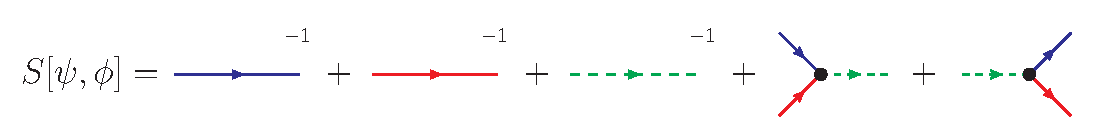
\includegraphics[width=\textwidth]{figs/action.pdf}
	\caption[Single-channel model]{Diagrammatic representation of the single-channel model in Eq.~\eqref{eq:single-channel-action}.
	The two classical fermion propagators are denoted by the blue and red full line, and the classical boson propagator is denoted by the green dashed line.}
	\label{fig:single-channel-model}
\end{figure}


\begin{figure}[b]
	\centering
	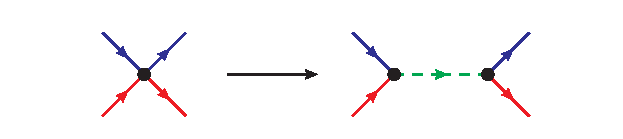
\includegraphics[width=0.6\textwidth]{figs/interaction.pdf}
	\caption[Microscopic interaction]{Diagrammatic representation of the Hubbard-Stratonovich transformation. The four-fermion interaction is modeled by the exchange of a bosonic dimer.}
	\label{fig:interaction}
\end{figure}


\section{Mean-field description} %%% or mean-field theory?
\label{section:nambu-gorkov-formalism}

Before diving into the fully non-perturbative description of the BCS-BEC crossover, it is worth investigating the theory on a mean-field level to get some physical intuition and to introduce the basic notation. In this context, the Nambu-Gorkov formalism~\cite{Boettcher2012} comes in handy, which is also used in other theories of superconductivity~\cite{Strinati2018}. This will also provide us with the mean-field propagators which will be used as initial guess for further computations. Let us define the Nambu spinors in momentum space, with $Q=(\omega_n,\bm{q})$,
%
\begin{align}
	\label{eq:nambu-spinors}
	\Psi^{\dagger}(Q) = \left(\psi_{\uparrow}^*(Q), \, \psi_{\downarrow}(-Q)\right) \,, \quad
	\Psi(Q) = \begin{pmatrix}\psi_{\uparrow}(Q) \\ \psi_{\downarrow}^*(-Q)\end{pmatrix} \,.
\end{align}
%
With these spinors, the fermionic part of the action~\eqref{eq:single-channel-action} can be written as
%
\begin{align}
	\label{eq:fermionic-action}
	S_F[\Psi] = \int_{0}^{\beta} d\tau \int d^3 x\,\, \Psi^{\dagger}
	\begin{pmatrix} \partial_{\tau}-\nabla^2-\mu  & h\phi \\
	h\phi^* & \partial_{\tau}+\nabla^2+\mu \end{pmatrix}
	\Psi \,.
\end{align}
%
From this expression, the inverse classical propagator $S^{(2)}_{\Psi\Psi^{\dagger}}(Q,Q')$
with constant background field $\Delta = h\phi$ can be derived~\cite{Diehl2010}
%
\begin{align}
	\label{eq:fermion-propagator}
	S^{(2)}_{\Psi\Psi^{\dagger}}(Q,Q') = \frac{\delta^2 S_F}{\delta\Psi(Q)\delta\Psi^{\dagger}(Q')} 
	= \delta(Q-Q')
	\begin{pmatrix} -i\omega_n+\varepsilon_{\bm{q}}-\mu & \Delta \\
	\Delta^* & -i\omega_n-\varepsilon_{\bm{q}}+\mu \end{pmatrix} \,,
\end{align}
%
where we defined the classical momentum dispersion $\varepsilon_{\bm{q}}=\bm{q}^2$. The parameter $\Delta$ is often called the gap parameter. A more detailed derivation of the propagators can be found in Appendix~\ref{app:propagators}. Note that a propagator comes always with an energy-momentum conserving delta function $G(Q,Q')=\delta(Q-Q')G(Q)$. In the following, we will call $G(Q)$ the propagator. From Eq.~\eqref{eq:fermion-propagator}, the classical fermion propagator, or BCS propagator, can be obtained via matrix inversion~\cite{VanLoon2020}
\begin{align}
	\label{eq:bcs-propagator}
	G^{(0)}_{\Psi\Psi^{\dagger}}(Q) = \frac{1}{\omega_n^2+\xi_{\bm{q}}^2+\Delta^2}
	\begin{pmatrix} i\omega_n+\xi_{\bm{q}} & \Delta \\
	\Delta^* & i\omega_n-\xi_{\bm{q}} \end{pmatrix} \,,
\end{align}
where $\xi_{\bm{q}}=\varepsilon_{\bm{q}}-\mu$. The components of the BCS propagator can be rewritten in terms of the Bogoliubov coefficients $u_{\bm{q}}, v_{\bm{q}}$ and a new BCS dispersion relation $E_{\bm{q}}=\sqrt{\xi_{\bm{q}}^2+\Delta^2}$,
%
\begin{align}
	\label{eq:bogoliubov-coefficients}
	u_{\bm{q}}^2 = \frac{1}{2}\left[1 + \frac{\xi_{\bm{q}}}{E_{\bm{q}}}\right] \,, \quad
	v_{\bm{q}}^2 = \frac{1}{2}\left[1 - \frac{\xi_{\bm{q}}}{E_{\bm{q}}}\right] \,, \quad
	u_{\bm{q}} v_{\bm{q}} = \frac{\Delta}{2E_{\bm{q}}} \,.
\end{align}
%
We call the diagonal entries of the propagator ($\uparrow\uparrow$, $\downarrow\downarrow$) the normal components,
%
\begin{align}
	\label{eq:normal-components}
	G^{(0)}_{\uparrow\uparrow}(Q) = \frac{i\omega_n+\xi_{\bm{q}}}{\omega_n^2+E_{\bm{q}}^2} = \frac{u_{\bm{q}}^2}{-i\omega_n+E_{\bm{q}}} + \frac{v_{\bm{q}}^2}{-i\omega_n-E_{\bm{q}}}	= - G^{(0)}_{\downarrow\downarrow}(-Q) \,,
\end{align}
%
and the off-diagonal entries ($\uparrow\downarrow$, $\downarrow\uparrow$) the anomalous components,
%
\begin{align}
	\label{eq:anomalous-components}
	G^{(0)}_{\uparrow\downarrow}(Q) = \frac{\Delta}{\omega_n^2+E_{\bm{q}}^2} = u_{\bm{q}} v_{\bm{q}}
	\left[\frac{1}{-i\omega_n+E_{\bm{q}}} - \frac{1}{-i\omega_n-E_{\bm{q}}}\right] = G^{(0)}_{\downarrow\uparrow}(Q) \,.
\end{align}
%
In the last equation, we chose $\Delta$ to be real without loss of generality~\cite{Fetter1971}.

The physical meaning of these components is very intuitive. In the normal phase where there is no condensate, i.e. $\Delta=0$, the off-diagonal components are zero and we are left with a standard fermionic propagator with classical dispersion relation. In the symmetry-broken phase, or superfluid phase, the gap parameter is non-zero ($\Delta\neq 0$) and we obtain a modified BCS dispersion relation, see Fig.~\ref{fig:dispersion-relation}. Thus, the anomalous components are directly related to the presence of a condensate field~\cite{Fetter1971}.

From Eq.~\eqref{eq:normal-components} and~\eqref{eq:anomalous-components}, the general initial spectral functions can be derived,
%
\begin{align}
	\label{eq:initial-spectral-functions}
	\rho^{(0)}_{\uparrow\uparrow}(\lambda,\bm{q}) &= u_{\bm{q}}^2\, \delta(\lambda-E_{\bm{q}}) + v_{\bm{q}}^2\, \delta(\lambda+E_{\bm{q}}) \,, \\
	\rho^{(0)}_{\uparrow\downarrow}(\lambda,\bm{q}) &= u_{\bm{q}} v_{\bm{q}} \left[\delta(\lambda-E_{\bm{q}}) - \delta(\lambda+E_{\bm{q}})\right] \,.
\end{align}
%
In the normal phase ($\Delta=0$), the spectral functions simplify to
%
\begin{align}
	\label{eq:normal-spectral-functions}
	\rho^{(0)}_{\uparrow\uparrow}(\lambda,\bm{q}) &= \delta(\lambda-\bm{q}^2+\mu) \,, \\
	\rho^{(0)}_{\uparrow\downarrow}(\lambda,\bm{q}) &= 0 \,.
\end{align}
%
Since the diagonal components, as well as the off-diagonal components, are related to each other for the spin- and mass-balanced Fermi gas, the system is completely described by one normal and one anomalous spectral function. Note that the anomalous spectral function satisfies the sum rules~\cite{Pieri2004-1}
%
\begin{align}
	\label{eq:anomalous-sum-rules}
	\int_{-\infty}^{\infty} d\lambda\, \rho_{\uparrow\downarrow}(\lambda,\bm{p}) &= 0 \,, \\
	\int_{-\infty}^{\infty} d\lambda\,\lambda\, \rho_{\uparrow\downarrow}(\lambda,\bm{p}) &= \Delta \,.
\end{align}
%
In the single-channel model, the bosonic dimer acts as an interaction exchange particle and has no classical dispersion relation. Thus, it has no clear interpretation as a probability distribution and is not normalized. In this way, it carries also no contribution to the total density. For a more detailed discussion of dynamic bosons within the two-channel model, see~\cite{Diehl2006-1,Diehl2007,Schmidt2013}.


\begin{figure}[b]
	\centering
	\subfigure[]{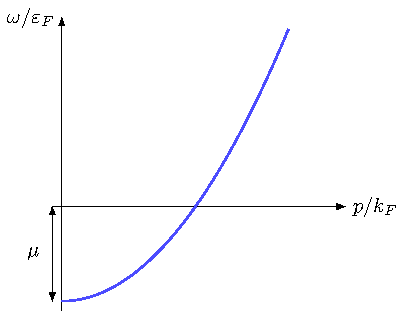
\includegraphics[width=0.42\textwidth]{figs/dispersion1.pdf}} 
	\subfigure[]{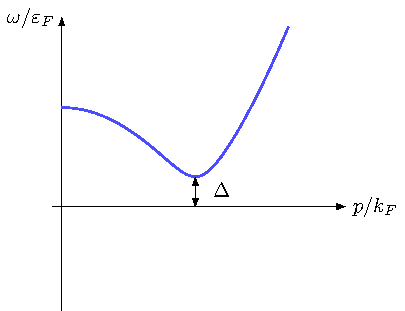
\includegraphics[width=0.42\textwidth]{figs/dispersion2.pdf}}
	\caption[Dispersion relations]{(a) Classical dispersion relation in the normal phase vs. (b) BCS dispersion relation in the superfluid phase.}
	\label{fig:dispersion-relation}
\end{figure}
	\chapter{BCS-BEC Crossover}
\label{chapter:bcs-bec-crossover}

In this Chapter, we investigate the spectral properties of the BCS-BEC crossover and present the main results of this work. A fully non-perturbative functional method~\cite{Horak2020} is applied to obtain spectral functions directly in real-time. We start with a simplified discussion of the normal phase and then present the general treatment in the superfluid phase. Numerical results of this work are compared to other approaches and existing results from the literature. In the end, the numerical framework is applied to describe recent experimental data from MIT~\cite{Mukherjee2019}.


\section{Normal phase}
\label{section:normal-phase}

Let us start with a discussion of the normal phase of the BCS-BEC crossover and introduce the basic concepts of the selfconsistent framework. As mentioned before, we are dealing with a balanced system in which the propagators of the $\uparrow$ and $\downarrow$ species are the same and we are left with only one fermion propagator $G_{\psi\psi^*} = G_{\psi_{\uparrow}\psi_{\uparrow}^*} = G_{\psi_{\downarrow}\psi_{\downarrow}^*}$. Since we are restricting ourselves to the normal phase, the gap parameter $\Delta$ is zero and the matrix propagator is diagonal. The Dyson-Schwinger equations for this system can be derived from the master DSE~\eqref{eq:DSE-general} by using the single-channel action in Eq.~\eqref{eq:single-channel-action}. Schematically, the fermion DSE reads
%
\begin{align}
	\label{eq:fermion-DSE}
	\Gamma^{(2)}_{\psi\psi^*} = S^{(2)}_{\psi\psi^*}
	+ S^{(3)}_{\psi^*_{\downarrow}\psi^*_{\uparrow}\phi} \cdot G_{\phi\phi^*}
	\cdot \Gamma^{(3)}_{\psi_{\uparrow}\psi_{\downarrow}\phi^*}
	\cdot G_{\psi\psi^*}  \,,
\end{align}
%
where $G_{\phi\phi^*}$ and $G_{\psi\psi^*}$ are the full boson and fermion propagators, and $S^{(3)}$ and $\Gamma^{(3)}$ are the classical and full vertices, respectively. The boson DSE reads analogously
%
\begin{align}
	\label{eq:boson-DSE}
	\Gamma^{(2)}_{\phi\phi^*} = S^{(2)}_{\phi\phi^*}
	- S^{(3)}_{\psi_{\downarrow}\psi_{\uparrow}\phi^*} \cdot G_{\psi\psi^*}
	\cdot \Gamma^{(3)}_{\psi^*_{\uparrow}\psi^*_{\downarrow}\phi}
	\cdot G_{\psi\psi^*}  \,.
\end{align}
%
Note the different sign from the fermionic loop. For a detailed derivation of the above equations, we refer the reader to Appendix~\ref{app:derivation-dse}.
The classical inverse propagators can be obtained from the microscopic action~\eqref{eq:single-channel-action}, see Appendix~\ref{app:propagators},
%
\begin{align}
	\label{eq:classical-propagators}
	S^{(2)}_{\psi\psi^*} = -i\omega_n+\bm{p}^2-\mu \,, \qquad
	S^{(2)}_{\phi\phi^*} = \nu \,.
\end{align}
%
The coupled Dyson-Schwinger equations for the fermion and boson propagator are depicted diagrammatically in Fig.~\ref{fig:prop_DSEs}. In this way, quantum fluctuations are included in the calculation and the classical propagators are related to the full ones. The full vertex $\Gamma^{(3)}$ could be included in principle, as has been done in~\cite{Horak2020}, but for this work it is approximated by the classical vertex, i.e. $\Gamma^{(3)}=S^{(3)}$. Referring to Section~\ref{section:single-channel-model}, we note that this approximation corresponds to a theory without background interaction, i.e., there is no quantum correction to the classical vertex without a background four-fermion coupling~\cite{Diehl2006-1}. Thus, this truncation is equivalent to the well-known T-matrix approach from the literature~\cite{Haussmann2007,Hanai2013}. However, the functional method can be generalized straightforwardly by taking the full three-point function $\Gamma^{(3)}$ into account.

\begin{figure}[t]
	\begin{center}
		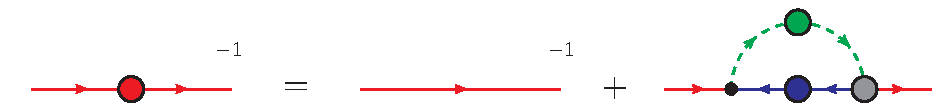
\includegraphics[width=0.8\textwidth]{figs/fermion_prop_DSE.pdf} \\
		\vspace{0.5cm}
		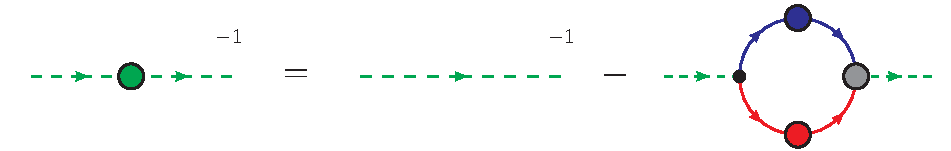
\includegraphics[width=0.8\textwidth]{figs/boson_prop_DSE.pdf} 
	\end{center}
	\caption[Coupled Dyson-Schwinger equations]{Coupled Dyson-Schwinger equations for the fermion and boson propagator. The red, blue and green blobs denote the full fermion and boson propagators. The black dot denotes the classical vertex $S^{(3)}$ and the gray blob denotes the full vertex $\Gamma^{(3)}$.}
	\label{fig:prop_DSEs}
\end{figure}

Inserting the classical propagators and the renormalized detuning from Eq.~\eqref{eq:renormalized-detuning} into the Dyson-Schwinger equations above yields the central equations of this work. Renaming the fermion propagator $G_{\psi} = G_{\psi\psi^*}$ and using $G^{-1}_{\psi} = \Gamma^{(2)}_{\psi\psi^*}$ and similarly for the boson gives
%
\begin{align}
	\label{eq:selfconsistent-equations}
	G^{-1}_{\psi}(\omega_n,\bm{p}) &= -i\omega_n+\bm{p}^2-\mu + \Sigma_{\psi}(\omega_n,\bm{p}) \,, \notag \\
	G^{-1}_{\phi}(\omega_n,\bm{p}) &= -\frac{h^2}{8\pi a} - \Pi_{\phi}(\omega_n,\bm{p}) \,,
\end{align}
%
where we defined the fermionic and bosonic self-energy, $\Sigma_{\psi}$ and $\Pi_{\phi}$, respectively. Using the classical Yukawa coupling $h$ for the vertices, the self-energies are given by
%
\begin{align}
	\label{eq:self-energies}
	\Sigma_{\psi}(\omega_n,\bm{p}) &= h^2 \int\frac{d^{3}q}{(2\pi)^{3}}\,T\sum_{\Omega_m} G_{\phi}(\Omega_m,\bm{q}) G_{\psi}(\Omega_m-\omega_n,\bm{q-p}) \,, \notag \\
	\Pi_{\phi}(\omega_n,\bm{p}) &= h^2 \int\frac{d^{3}q}{(2\pi)^{3}}\left[ T\sum_{\Omega_m} G_{\psi}(\Omega_m,\bm{q}) G_{\psi}(\omega_n-\Omega_m,\bm{p-q}) - \frac{1}{2\bm{q}^2} \right] \,,
\end{align}
%
where the last term was absorbed from the renormalized detuning to regularize the integral. Note that in the fermionic self-energy $\Sigma_{\psi}$, the sum is over bosonic Matsubara frequencies $\Omega_m=2m\pi T$, whereas in the bosonic self-energy $\Pi_{\phi}$, the sum is over fermionic Matsubara frequencies $\Omega_m=(2m+1)\pi T$.

Using the spectral representation in Eq.~\eqref{eq:spectral-representation} for the fermion and boson propagator, the self-energies can be written in terms of spectral loop integrals, 
%
\begin{align}
	\label{eq:spectral-self-energies}
	\Sigma_{\psi}(\omega_n,\bm{p}) &= h^2\int_{\bm{q},\lambda_1,\lambda_2}
	\rho_{\phi}(\lambda_1,\bm{q}) \rho_{\psi}(\lambda_2,\bm{q}-\bm{p})\,
	I_{\psi}(\omega_n,\lambda_1,\lambda_2) \,, \notag \\
	\Pi_{\phi}(\omega_n,\bm{p}) &= h^2\int_{\bm{q}} \left[\int_{\lambda_1,\lambda_2}
	\rho_{\psi}(\lambda_1,\bm{q}) \rho_{\psi}(\lambda_2,\bm{p}-\bm{q})\,
	I_{\phi}(\omega_n,\lambda_1,\lambda_2) - \frac{1}{2\bm{q}^2} \right] \,.
\end{align}
%
We use the notation $\int_{\bm{q}}=\int d^3q/(2\pi)^3$ and $\int_{\lambda}=\int_{-\infty}^{\infty}d\lambda$. The Matsubara summation in $I_{\psi}(\omega_n,\lambda_1,\lambda_2)$ and $I_{\phi}(\omega_n,\lambda_1,\lambda_2)$ can be carried out analytically, leaving us with symbolic expressions in terms of the argument $\omega_n$ for both self-energies, which can be evaluated at any complex frequency. The explicit calculation of the Matsubara sums can be found in Appendix~\ref{app:matsubara-sums} and a more detailed discussion in~\cite{Punk2010}.

The resulting expressions for $I_{\psi}(\omega_n,\lambda_1,\lambda_2)$ and $I_{\phi}(\omega_n,\lambda_1,\lambda_2)$ are given by
%
\begin{align}
	\label{eq:spectral-sums}
	I_{\psi}(\omega_n,\lambda_1,\lambda_2) &= T\sum_{\Omega_m} \frac{1}{i\Omega_m-\lambda_1}\frac{1}{i(\Omega_m-\omega_n)-\lambda_2} = \frac{-n_B(\lambda_1)-n_F(\lambda_2)}{-i\omega_n+\lambda_1-\lambda_2} \,, \notag \\
	I_{\phi}(\omega_n,\lambda_1,\lambda_2) &= T\sum_{\Omega_m} \frac{1}{i\Omega_m-\lambda_1}\frac{1}{i(\omega_n-\Omega_m)-\lambda_2} = \frac{1-n_F(\lambda_1)-n_F(\lambda_2)}{-i\omega_n+\lambda_1+\lambda_2} \,,
\end{align}
%
where $n_F(\lambda)=1/(e^{\lambda/T}+1)$ is the Fermi distribution function and $n_B(\lambda)=1/(e^{\lambda/T}-1)$ is the Bose-Einstein distribution function. For $T\rightarrow0$, the results simplify according to $n_B(\lambda)\rightarrow-\theta(-\lambda)$ and $n_F(\lambda)\rightarrow\theta(-\lambda)$, where $\theta(\lambda)$ is the Heaviside step function.

%%%%%%%%%%%%%%%%%%%%%%%%%%%%
\subsection*{Evaluation at real frequencies}
\label{sec:evaluation-real-frequencies}

The regularized and coupled DSEs in~\eqref{eq:selfconsistent-equations} can be evaluated at arbitrary complex frequencies. For the extraction of the spectral functions with~\eqref{eq:spectral-relation}, we choose $\omega_n=-i(\omega+i\varepsilon)$ with $\omega$ real and $\varepsilon\rightarrow 0^+$. The limit $\varepsilon\rightarrow 0^+$ is performed analytically using the relation
%
\begin{align}
	\label{eq:principal-value}
	\frac{1}{x\pm i0^+} = P\frac{1}{x} \mp i\pi\delta(x) \,,
\end{align}
%
where $P$ denotes the principal value. The delta function eliminates one spectral integration which allows us to write the imaginary part of the retarded self-energies as
%
\begin{align}
	\label{eq:imaginary-part-self-energies}
	\mathrm{Im}\,\Sigma^R_{\psi}(\omega,\bm{p}) &= \pi h^2\int_{\bm{q},\lambda}
	\rho_{\phi}(\omega+\lambda,\bm{q}) \rho_{\psi}(\lambda,\bm{q}-\bm{p})
	\left[-n_B(\omega+\lambda)-n_F(\lambda)\right] \,, \notag \\
	\mathrm{Im}\,\Pi^R_{\phi}(\omega,\bm{p}) &= \pi h^2\int_{\bm{q},\lambda}
	\rho_{\psi}(\omega-\lambda,\bm{q}) \rho_{\psi}(\lambda,\bm{p}-\bm{q})
	\left[1-n_F(\omega-\lambda)-n_F(\lambda)\right] \,.
\end{align}
%
Note that the pole of $n_B(\omega+\lambda)$ in the fermion self-energy is exactly canceled by the zero crossing of the boson spectral function $\rho_{\phi}$, see Section~\ref{section:spectral-representation}.

The real part of the retarded self-energies is obtained very efficiently from the imaginary part via the Kramers-Kronig relation~\cite{Abrikosov1975,Veillette2008},
%
\begin{align}
	\label{eq:kramers-kronig}
	\mathrm{Re}\,\Sigma^R(\omega,\bm{p}) = \frac{1}{\pi}\, P\int_{\lambda} \frac{\mathrm{Im}\, \Sigma^R(\lambda,\bm{p})}{\lambda-\omega} \,,
\end{align}
%
avoiding the 4-dimensional integrals in~\eqref{eq:spectral-self-energies} and performing a controlled 1-di\-men\-sio\-nal principal value integral instead. The fermionic self-energy decays for large values of the argument $\lambda$, see Appendix~\ref{app:fermion-self-energy-calculation}. Thus, the Kramers-Kronig relation can be used without further manipulations to compute the real part. As we will see later, the bosonic self-energy grows indefinitely for large values of $\lambda$ and requires special subtraction schemes to treat the divergent parts analytically. This has to do with the counterterm in~\eqref{eq:spectral-self-energies} and is discussed in detail in Appendix~\ref{app:boson-self-energy-calculation}.

Having obtained the real and imaginary part of the retarded self-energies, the spectral functions can be calculated with Eq.~\eqref{eq:spectral-relation}. More explicitly, for the fermions,
%
\begin{align}
	\label{eq:spectral-extraction}
	\rho_{\psi}(\omega,\bm{p}) = \frac{1}{\pi}\, \mathrm{Im}\, G^R_{\psi}(\omega,\bm{p}) = \frac{-\mathrm{Im}\,\Sigma^R_{\psi}(\omega,\bm{p})/\pi}{\left[\omega-\bm{p}^2+\mu-\mathrm{Re}\,\Sigma^R_{\psi}(\omega,\bm{p})\right]^2+\left[\mathrm{Im}\, \Sigma^R_{\psi}(\omega,\bm{p})\right]^2} \,.
\end{align}
%
This updated spectral function can be used in the next iteration to solve the coupled DSEs in Fig.~\ref{fig:prop_DSEs} selfconsistently until convergence is reached.


%%%%%%%%%%%%%%%%%%%%%%%%%%%%
\subsection*{First iteration of the boson self-energy}
\label{sec:first-iteration}

The iterative procedure is initialized with the first iteration of the boson self-energy, for which analytic results at finite and zero temperature can be derived. Inserting the classical fermion spectral function $\rho_{\psi}(\lambda,\bm{p})=\delta(\lambda-\bm{p}^2+\mu)$ in Eq.~\eqref{eq:spectral-self-energies} and performing the spectral integrals, we obtain the well-known expression for the non-selfconsistent retarded boson self-energy
%
\begin{align}
	\label{eq:non-selfconsistent-boson-self-energy}
	\Pi^R_{\phi}(\omega,\bm{p}) = h^2 \int_{\bm{q}}\left[ \frac{1-n_F(\varepsilon_{\bm{q}}-\mu) -n_F(\varepsilon_{\bm{p-q}}-\mu)}{-\omega+\varepsilon_{\bm{q}} + \varepsilon_{\bm{p-q}}-2\mu-i0^+} - \frac{1}{2\bm{q}^2}\right] \,,
\end{align}
%
where $\varepsilon_{\bm{p}}=\bm{p}^2$ is the classical momentum dispersion. At finite temperature, the imaginary part can be calculated analytically. The full calculation of the boson self-energy with general mass and spin-imbalance can be found in Appendix~\ref{app:boson-self-energy-calculation}. Here, we just state the result for the balanced case with equal mass and chemical potential.

For $y\geq 0$, the imaginary part at finite temperature is given by
%
\begin{align}
	\label{eq:boson-imaginary-part-finite-temp}
	\text{Im}\,\Pi^R_{\phi}(\omega,\bm{p}) = \frac{h^2}{8\pi} \left[ \sqrt{y} -
	\begin{cases}
		2\sqrt{y}\,n_F\left(y-\mu\right) & ,\, \bm{p}=\bm{0} \\
		\frac{T}{p} \ln\left( \frac{n_F(\mu-q_{+}^2)}{n_F(\mu-q_{-}^2)} \right) & ,\, \bm{p}\neq\bm{0}
	\end{cases} \right] \,,
\end{align}
%
where we have defined $y=\omega/2-p^2/4+\mu$ and $q_{\pm} = \sqrt{y}\pm p/2$, with $p=|\bm{p}|$. For $y<0$, the imaginary part vanishes identically. The real part at finite temperature cannot be solved analytically and has to be calculated numerically. However, at zero temperature, analytic expressions for both parts can be found. At $T=0$, the imaginary part is
%
\begin{align}
	\label{eq:boson-imaginary-part-zero-temp}
	\text{Im}\,\Pi^R_{\phi}(\omega,\bm{p}) = \frac{h^2}{8\pi} \left[ \sqrt{y} -
	\begin{cases}
		2\sqrt{y}\,\theta\left(\mu-y\right) & ,\, \bm{p}=\bm{0} \\
		\frac{\theta\left( \mu-
			q_{-}^2 \right)}{p} \left[
		\mu-q_{-}^2 -
		\left(\mu-q_{+}^2\right)
		\theta\left( \mu-q_{+}^2 \right)
		\right] & ,\, \bm{p}\neq\bm{0}
	\end{cases} \right] \,.
\end{align}
%
Note that the second term only contributes for $\mu>0$. The real part at vanishing spatial momentum, see Appendix~\ref{app:boson-self-energy-calculation}, is given for $\mu>0$ by
%
\begin{align}
	\label{eq:boson-real-part-zero-momentum}
	\text{Re}\, \Pi^R_{\phi}(\omega,\bm{0}) &= \frac{h^2}{2\pi^2} \left[ \sqrt{\mu} - \sqrt{|y|}
	\begin{cases}
		\text{arctanh}\left(\sqrt{\frac{\mu}{y}}\right) & ,\, y \geq 0 \\
		\arctan\left( \sqrt{\frac{\mu}{|y|}}\right)-\frac{\pi}{4} & ,\, y < 0
	\end{cases} \right]	\,.
\end{align}
%
For general non-zero spatial momentum, the expression is slightly more complicated
\begin{align}
	\label{eq:boson-real-part-general-momentum}
	\text{Re}\, \Pi^R_{\phi}(\omega,\bm{p}) =\,
	&\frac{h^2}{4\pi^2} \left[
	\sqrt{\mu} - \frac{y-\mu+p^2/4}{2p}\log\left(\frac{y-\tilde{q}^2_{+}}{y-\tilde{q}^2_{-}}\right)\right. \notag \\
	&- \sqrt{|y|}\left.
	\begin{cases}
		\text{arctanh}\left(\frac{\tilde{q}_{-}}{\sqrt{y}}\right) + 
		\text{arctanh}\left(\frac{\tilde{q}_{+}}{\sqrt{y}}\right) & ,\, y \geq 0 \\
		\text{arctan}\left(\frac{\tilde{q}_{-}}{\sqrt{|y|}}\right) +
		\text{arctan}\left(\frac{\tilde{q}_{+}}{\sqrt{|y|}}\right)-\frac{\pi}{2} & ,\, y < 0
	\end{cases}
	\right] \,,
\end{align}
with $\tilde{q}_{\pm} = \sqrt{\mu} \pm p/2$. For $\mu<0$, the real part is just given by $\text{Re}\, \Pi^R_{\phi}(\omega,\bm{p})=h^2\sqrt{-y}/(8\pi)$, where $y<0$. These results also agree with the formulas given in~\cite{Punk2010}.


\clearpage

\section{Superfluid phase}
\label{section:superfluid-phase}

In this Section, we consider the general case of a non-vanishing condensate expectation value ($\Delta\neq 0$). Now, we also have to account for the off-diagonal, also called anomalous, contributions. The general structure of the new DSEs is given by
%
\begin{align}
	\label{eq:matrix-DSE-structure}
	\begin{pmatrix}
		\Gamma^{(2)}_{11} & \Gamma^{(2)}_{12} \\
		\Gamma^{(2)}_{21} & \Gamma^{(2)}_{22}
	\end{pmatrix}
	=
	\begin{pmatrix}
		S^{(2)}_{11} & S^{(2)}_{12} \\
		S^{(2)}_{21} & S^{(2)}_{22}
	\end{pmatrix}
	-
	\begin{pmatrix}
		\Sigma_{11} & \Sigma_{12} \\
		\Sigma_{21} & \Sigma_{22}
	\end{pmatrix} \,,
\end{align}
%
and the components of the propagator are determined with Eq.~\eqref{eq:propagator-gamma} by a matrix inverse
%
\begin{align}
	\label{eq:matrix-propagator-inverse}
	\begin{pmatrix}
		G_{11} & G_{12} \\
		G_{21} & G_{22}
	\end{pmatrix}
	= \frac{1}{\Gamma^{(2)}_{11}\Gamma^{(2)}_{22}
		-\Gamma^{(2)}_{12}\Gamma^{(2)}_{21}}
	\begin{pmatrix}
		\Gamma^{(2)}_{22} & -\Gamma^{(2)}_{12} \\
		-\Gamma^{(2)}_{21} & \Gamma^{(2)}_{11}
	\end{pmatrix} \,.
\end{align}
%
This means that the fermion and boson propagators are now matrix objects with normal and anomalous components. For the balanced case, we choose the notation
%
\begin{align}
	\label{eq:matrix-propagators-components}
	G_{\Psi\Psi^{\dagger}} =
	\begin{pmatrix}
		G_{\uparrow\uparrow} & G_{\uparrow\downarrow} \\
		G_{\downarrow\uparrow} & G_{\downarrow\downarrow}
	\end{pmatrix} \,, \qquad
	G_{\Phi\Phi^{\dagger}} =
	\begin{pmatrix}
		G_{\phi\phi^*} & G_{\phi\phi} \\
		G_{\phi^*\phi^*} & G_{\phi^*\phi}
	\end{pmatrix} \,.
\end{align}
%
Owing to the symmetry identities introduced in Section~\ref{section:nambu-gorkov-formalism}, the only independent components for the balanced Fermi gas are $G_{\uparrow\uparrow}$, $G_{\uparrow\downarrow}$, $G_{\phi\phi^*}$ and $G_{\phi\phi}$. Thus, each propagator is described completely by one normal and one anomalous component. Consequently, we now have four, instead of two, coupled equations, i.e., the normal components also depend on the anomalous components. For more details, also on the more general spin-imbalanced case, see~\cite{Frank2018}. The additional DSEs for the anomalous components can be derived by the same means from the master DSE in Eq.~\eqref{eq:DSE-general}, see Appendix~\ref{app:derivation-dse}. Using the new notation, the fermion DSEs in the symmetry-broken phase are given by\footnote{Note the different sign as compared to~\cite{Haussmann2009} for the anomalous component, see also~\cite{Andrenacci2003,Frank2018,Pieri2004-1}.}
%
\begin{align}
	\label{eq:fermion-DSEs-general}
	\Gamma^{(2)}_{\uparrow\uparrow}(P) &= S^{(2)}_{\uparrow\uparrow}(P) + h^2 \int_Q G_{\phi\phi^*}(Q) \cdot G_{\uparrow\uparrow}(Q-P)  \,, \notag \\
	\Gamma^{(2)}_{\uparrow\downarrow}(P) &= S^{(2)}_{\uparrow\downarrow}(P) - h^2 \int_Q G_{\phi\phi}(Q) \cdot G_{\uparrow\downarrow}(Q-P) \,,
\end{align}
%
where $P=(\omega_n,\bm{p})$ and $\int_Q=T\sum_{\Omega_n}\int_{\bm{q}}$. Analogously, the boson DSEs are given by
%
\begin{align}
	\label{eq:boson-DSEs-general}
	\Gamma^{(2)}_{\phi\phi^*}(P) &= S^{(2)}_{\phi\phi^*}(P) - h^2 \int_Q G_{\uparrow\uparrow}(Q) \cdot G_{\uparrow\uparrow}(P-Q) \,, \notag \\
	\Gamma^{(2)}_{\phi\phi}(P) &= S^{(2)}_{\phi\phi}(P) + h^2 \int_Q G_{\uparrow\downarrow}(Q) \cdot G_{\uparrow\downarrow}(P-Q) \,.
\end{align}
%
The classical inverse fermion and boson Green's functions are given by
%
\begin{align}
	\label{eq:classical-propagators-components}
	S^{(2)}_{\Psi\Psi^{\dagger}} =
	\begin{pmatrix}
		-i\omega_n+\xi_{\bm{p}} & \Delta \\
		\Delta & -i\omega_n-\xi_{\bm{p}}
	\end{pmatrix} \,, \qquad
	S^{(2)}_{\Phi\Phi^{\dagger}} =
	\begin{pmatrix}
		\nu & 0 \\
		0 & \nu
	\end{pmatrix} \,.
\end{align}
%
For more details on the symmetries between the components and the evaluation at real frequencies, see Appendix~\ref{app:derivation-dse} and~\cite{Pieri2004-1}.


%%%%%%%%%%%%%%%%%%%%%%%%%%%%
\section{Results}
\label{section:results}

In this Section, we discuss the numerical results obtained in this work. In the first part, we focus on the novel results for the non-perturbative spectral functions calculated directly in real frequencies and compare with other approaches. In the following parts, we benchmark our method against existing results for the unitary Fermi gas and compare with experimental data from MIT~\cite{Mukherjee2019}.


\subsection*{Spectral functions}
\label{subsection:spectral-functions}

We start with a discussion of the results for the spin-balanced Fermi gas in the normal phase. For details on the numerical implementation, we refer the reader to Appendix~\ref{app:numerical-implementation}.

Physical properties and reconstructions of the fermion spectral function have been discussed extensively in the literature~\cite{Haussmann2009,Palestini2012,Reichl2015}. However, fully selfconsistent results obtained directly in real-time are limited. Simultaneously with the spectral approach developed in this work, there have been other unpublished works by Johannes Lang and Tilman Enss based on the Keldysh formalism. In particular, the code of Johannes Lang is based on a fast Fourier transform to real-times that renders the convolutions in the self-energy expressions to simple matrix multiplications~\cite{Lang2023}. It was originally developed for general dynamic systems out of equilibrium and will be used to compare with our results in thermal equilibrium. In this part, we also show the bosonic dimer spectral function which has not received much attention in the past.

\begin{figure*}[b]
	\centering
	\subfigure[$(k_Fa)^{-1}=-0.5$]{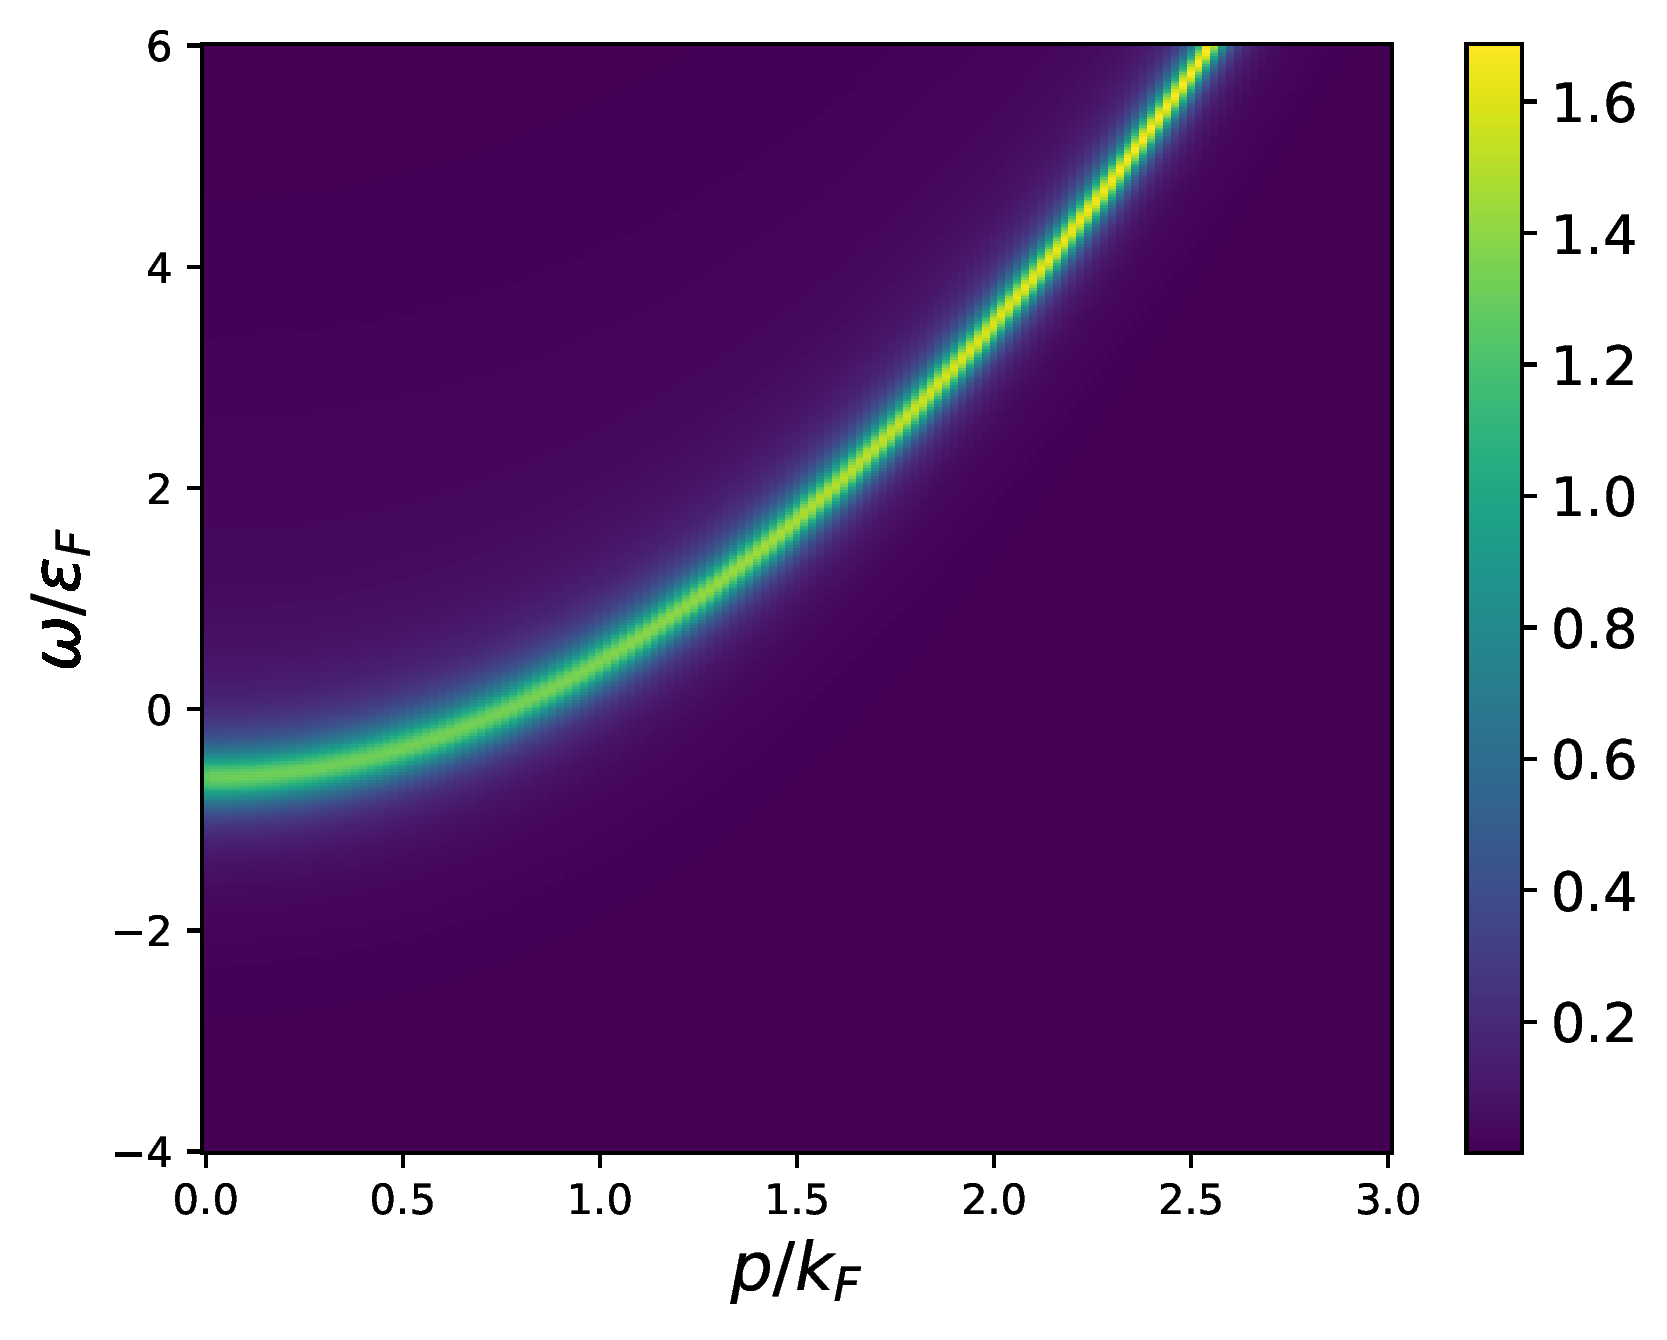
\includegraphics[width=0.32\textwidth]{figs/ferm_spec_kFa=-0.5.png}}
	\subfigure[$(k_Fa)^{-1}=0$]{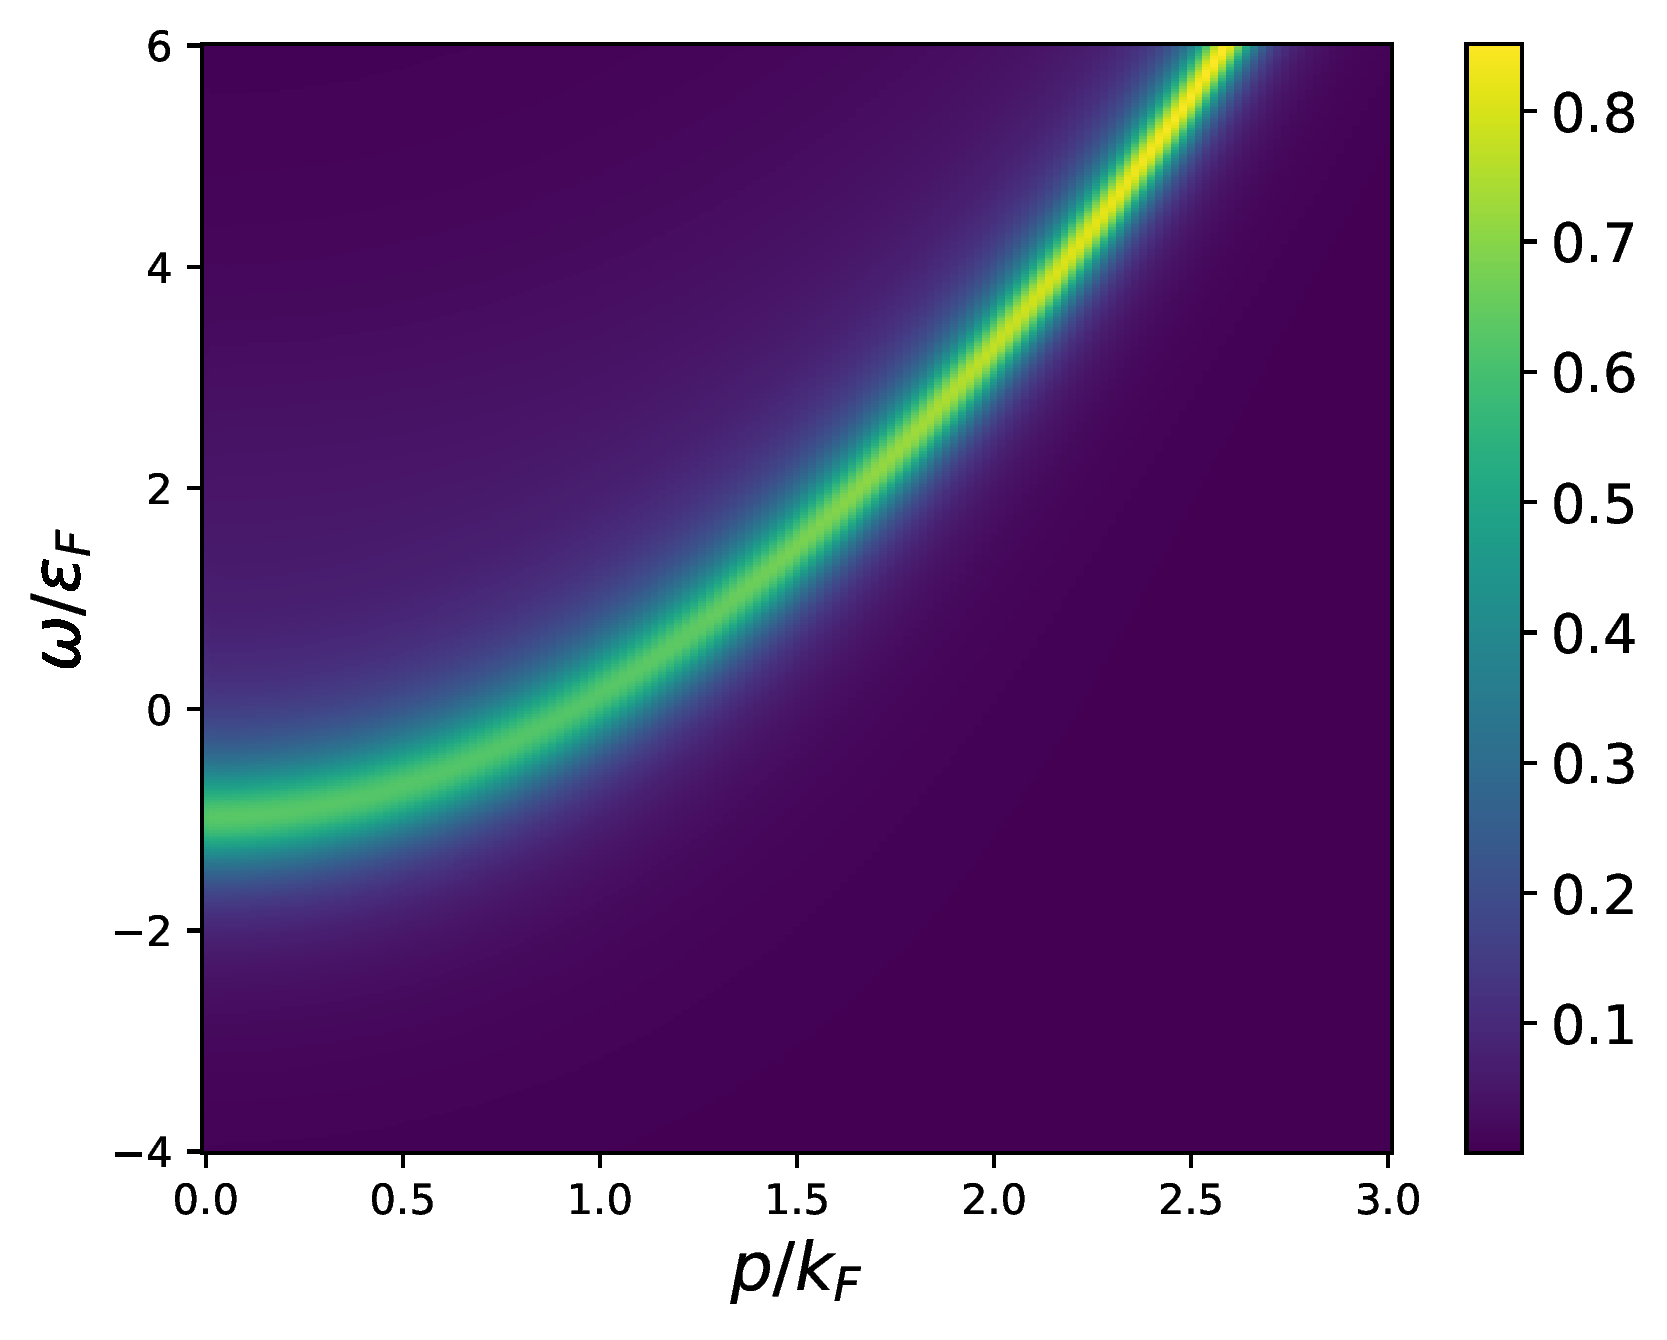
\includegraphics[width=0.32\textwidth]{figs/ferm_spec_kFa=0.png}}
	\subfigure[$(k_Fa)^{-1}=0.5$]{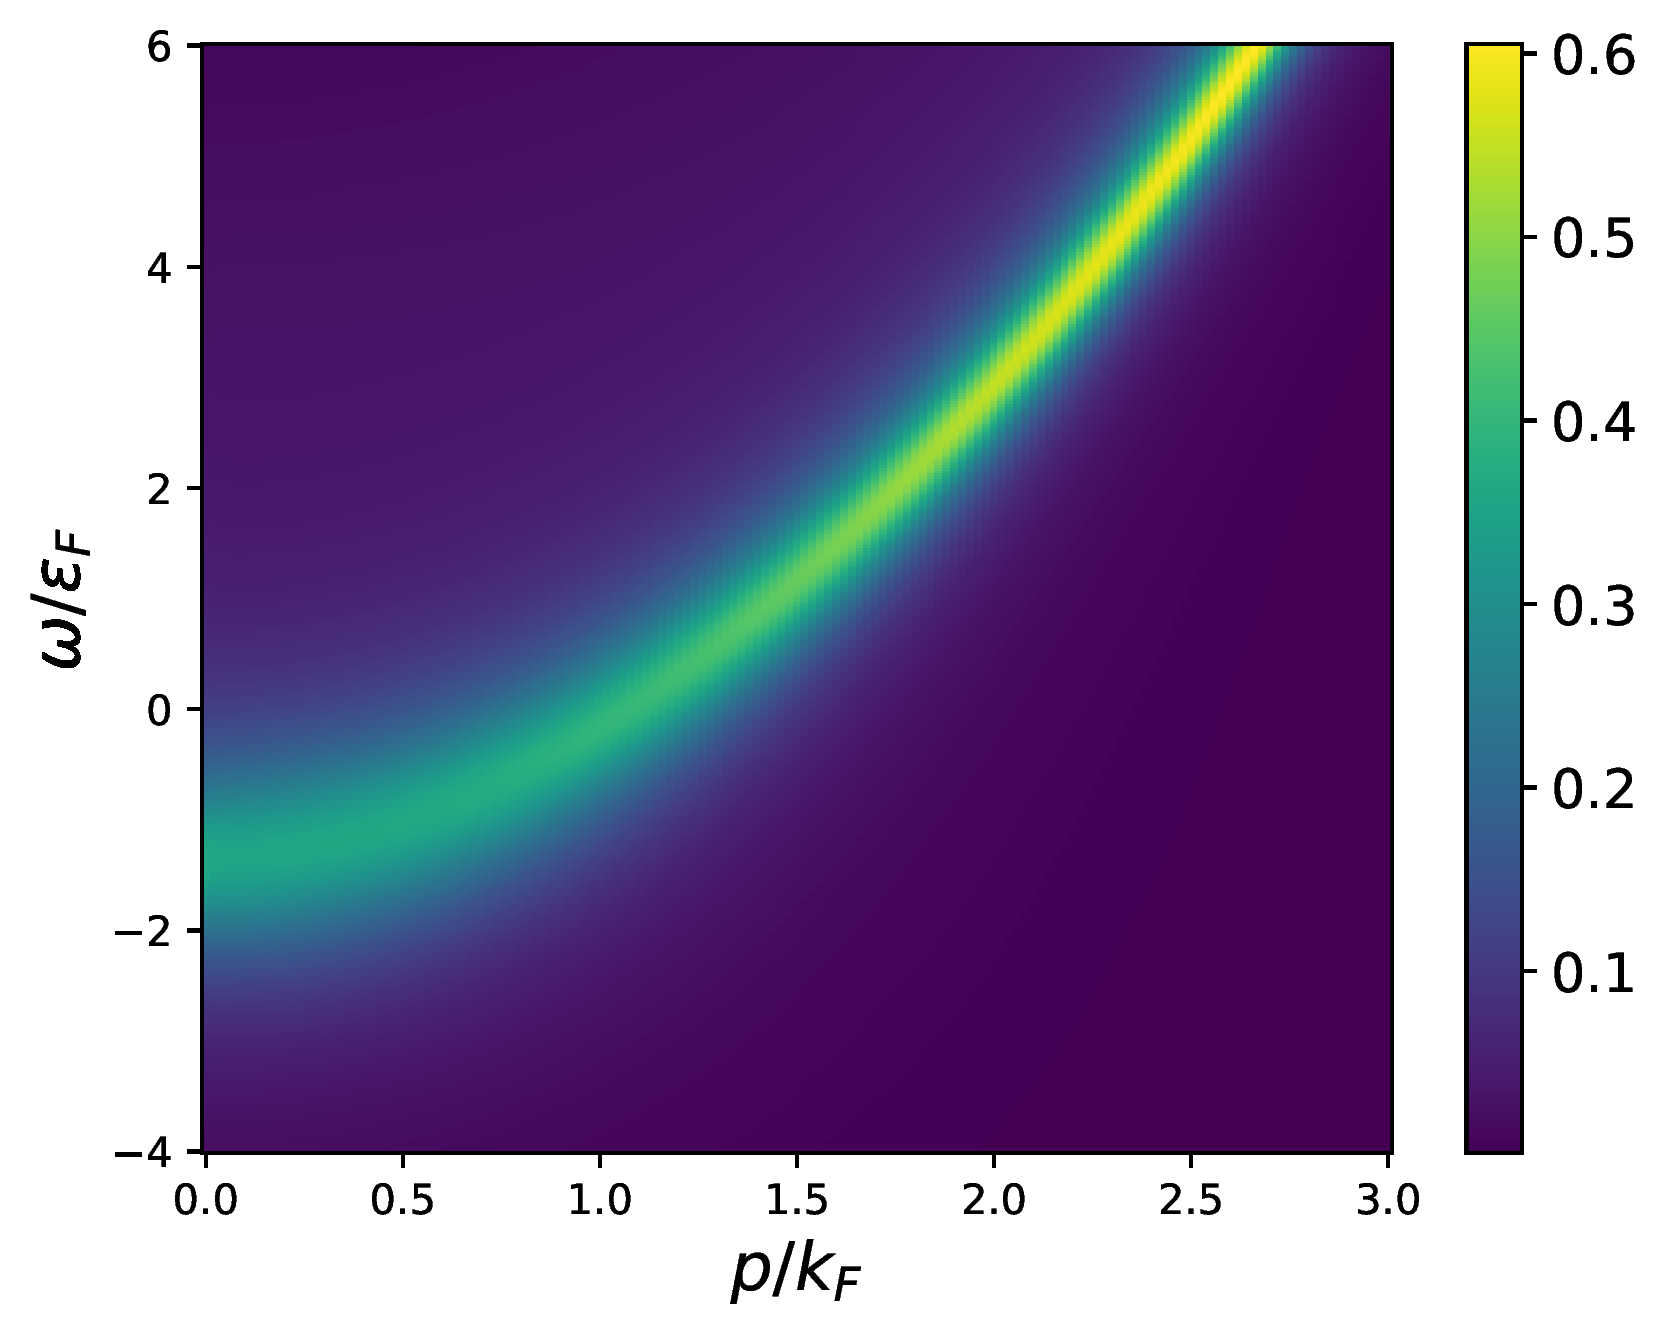
\includegraphics[width=0.32\textwidth]{figs/ferm_spec_kFa=0.5.png}}
	\caption[Fermion spectral function $\rho_{\psi}$ at different interaction strengths]{Results for the normalized fermionic spectral function $\rho_{\psi}\,\varepsilon_F$ for $\beta\mu=0.13146$ at different interaction strengths $(k_Fa)^{-1}$ which correspond to (a) BCS regime (b) unitarity (c) BEC regime.}
	\label{fig:fermion-specs}
\end{figure*}
%
\begin{figure*}[h]
	\centering
	\subfigure[$(k_Fa)^{-1}=-0.5$]{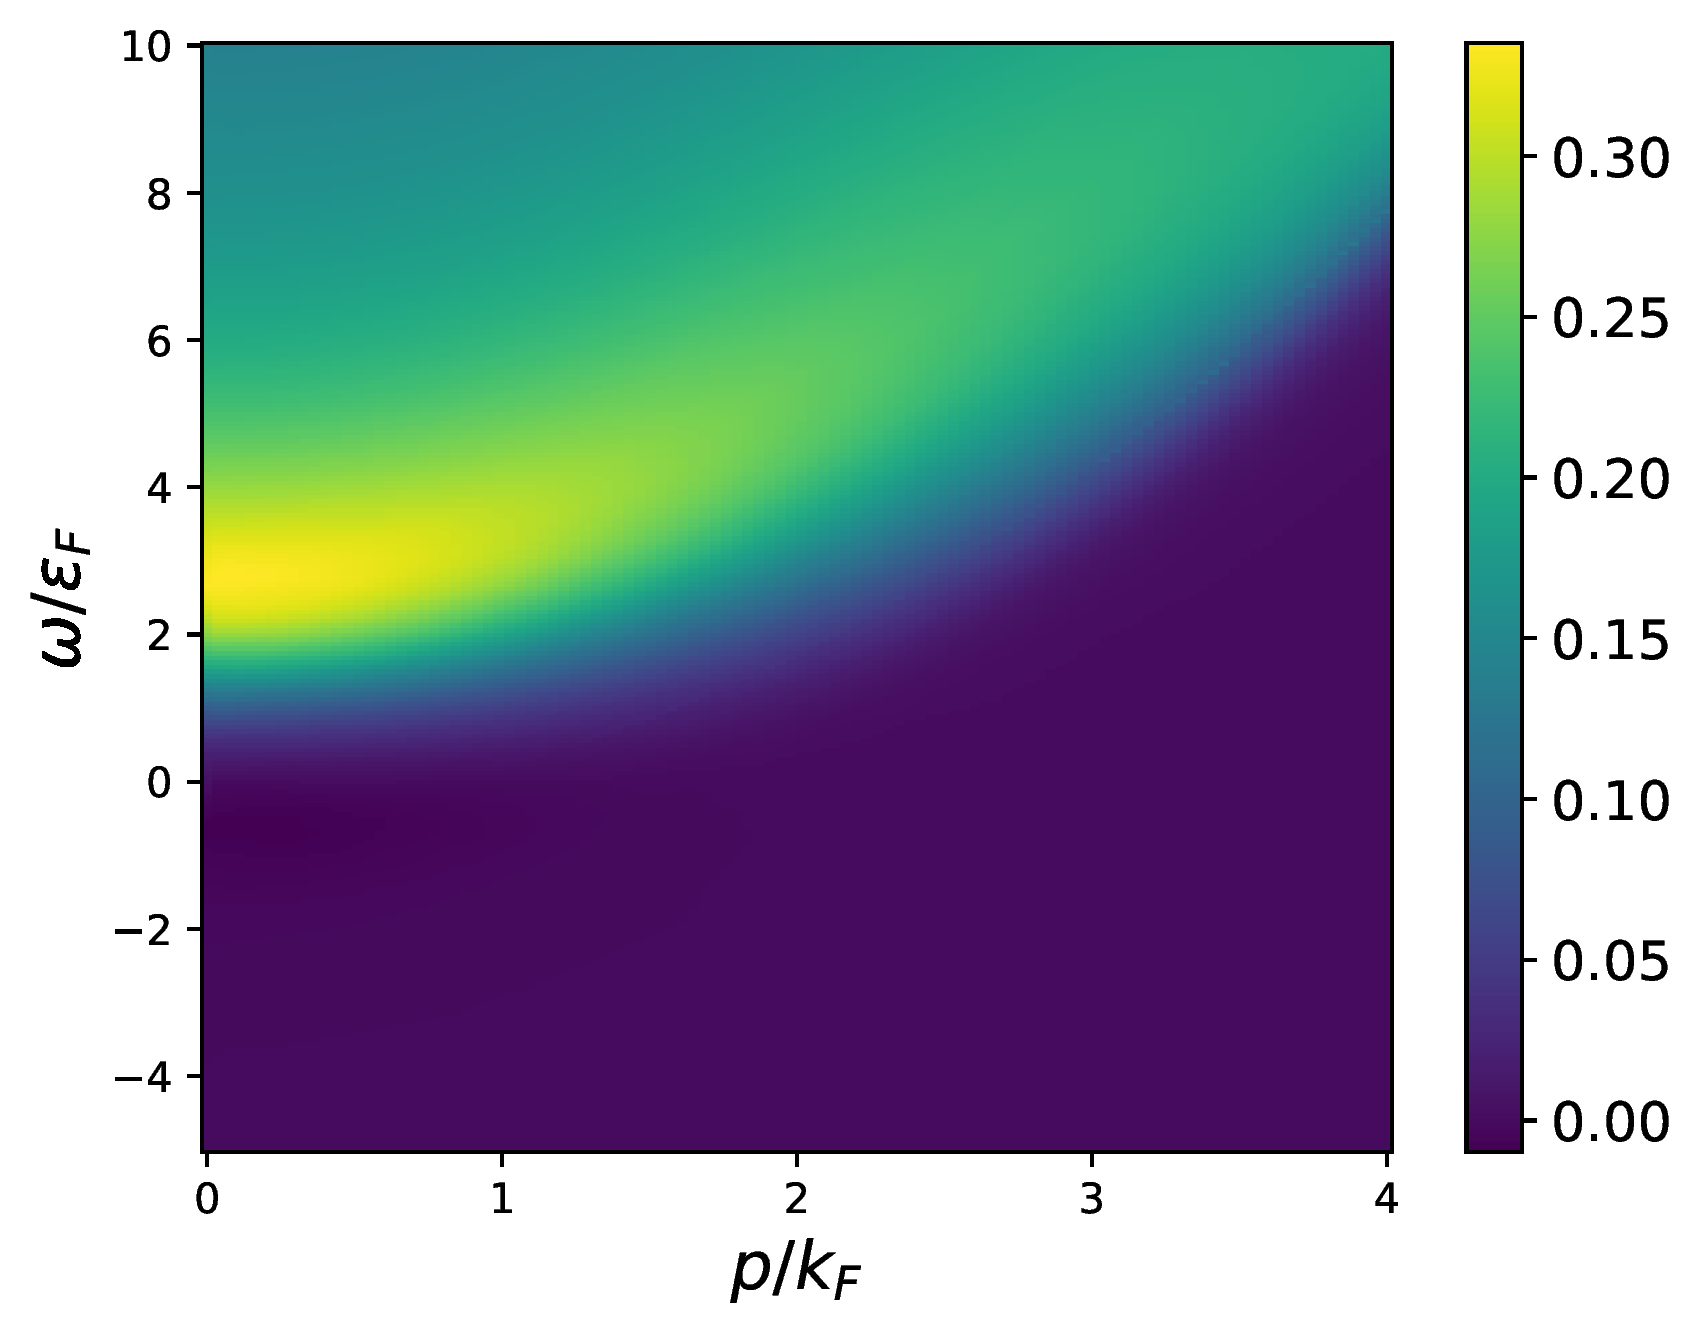
\includegraphics[width=0.328\textwidth]{figs/bos_spec_kFa=-0.5.png}}
	\subfigure[$(k_Fa)^{-1}=0$]{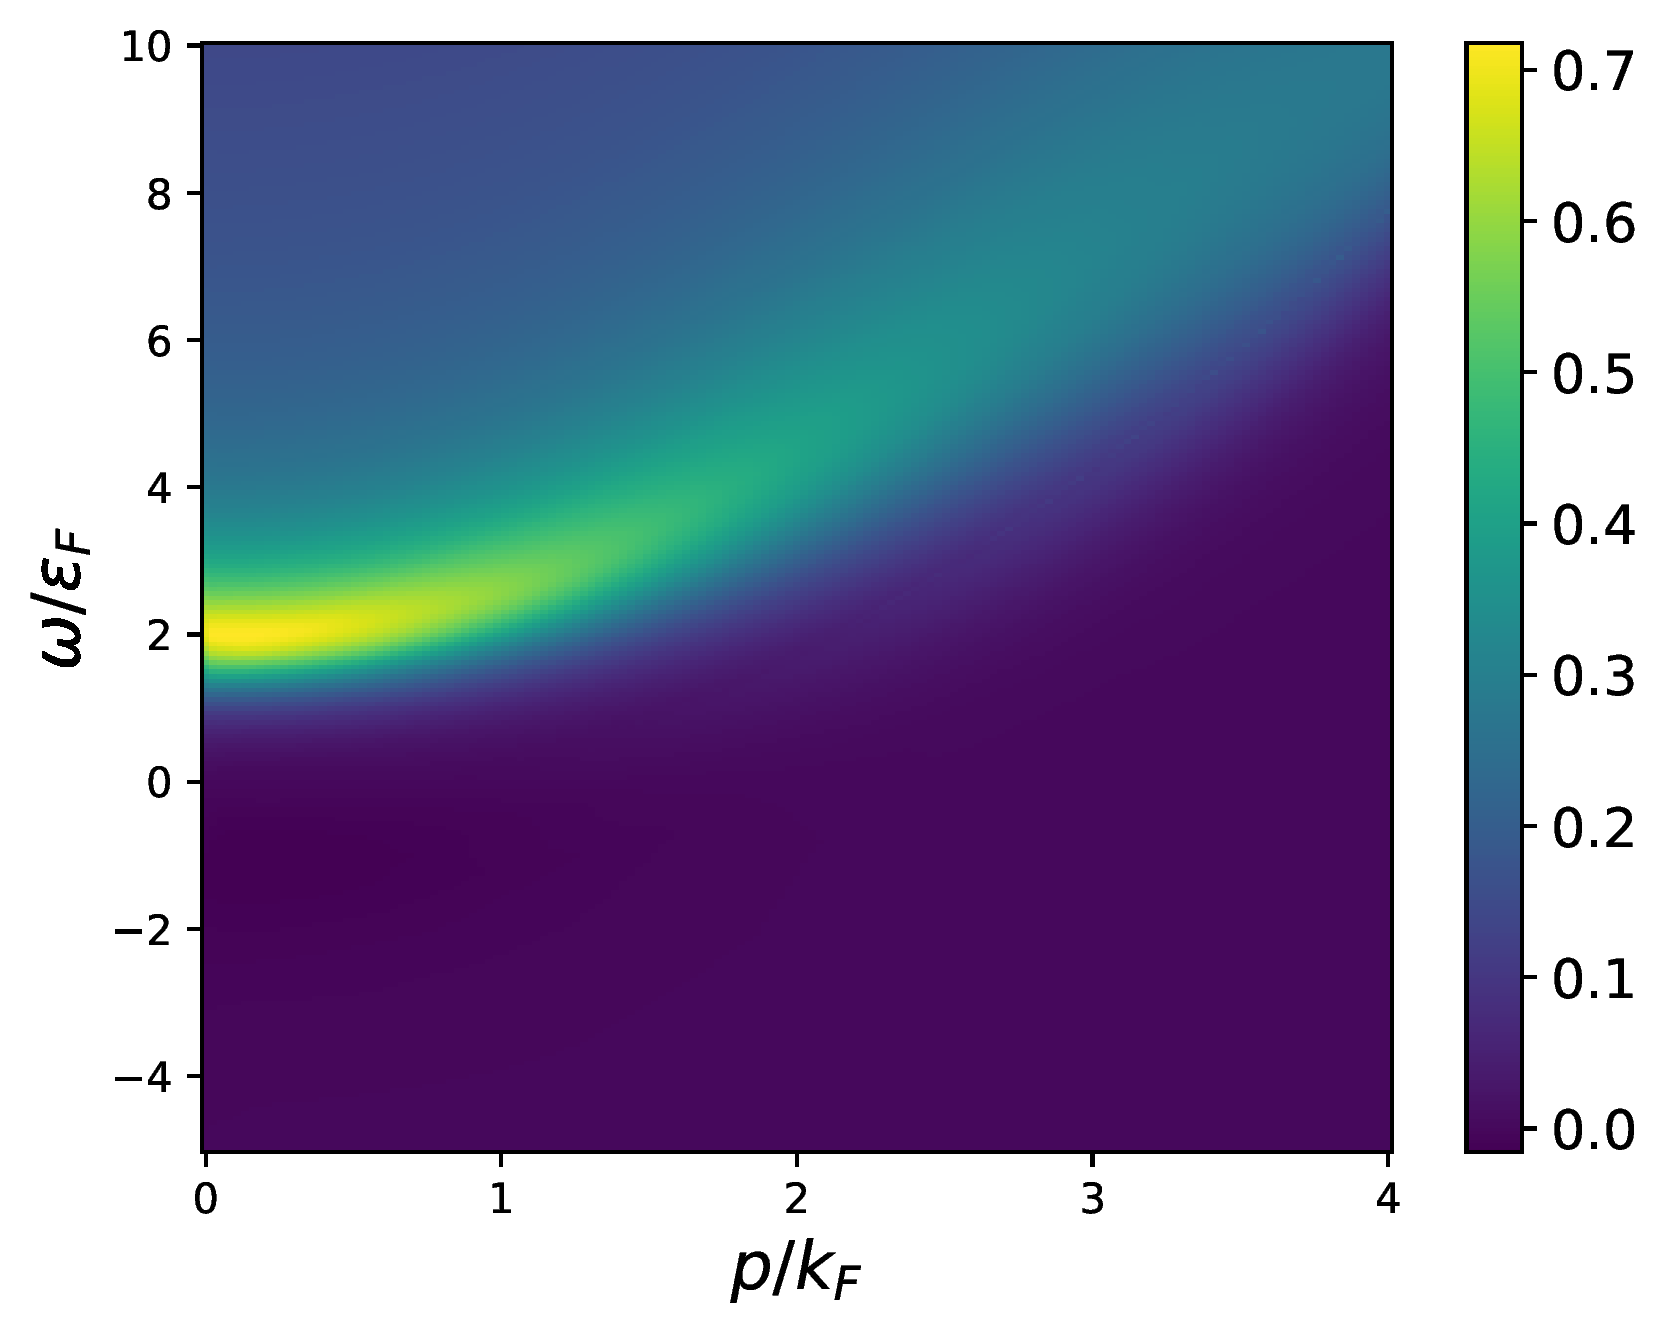
\includegraphics[width=0.32\textwidth]{figs/bos_spec_kFa=0.png}}
	\subfigure[$(k_Fa)^{-1}=0.5$]{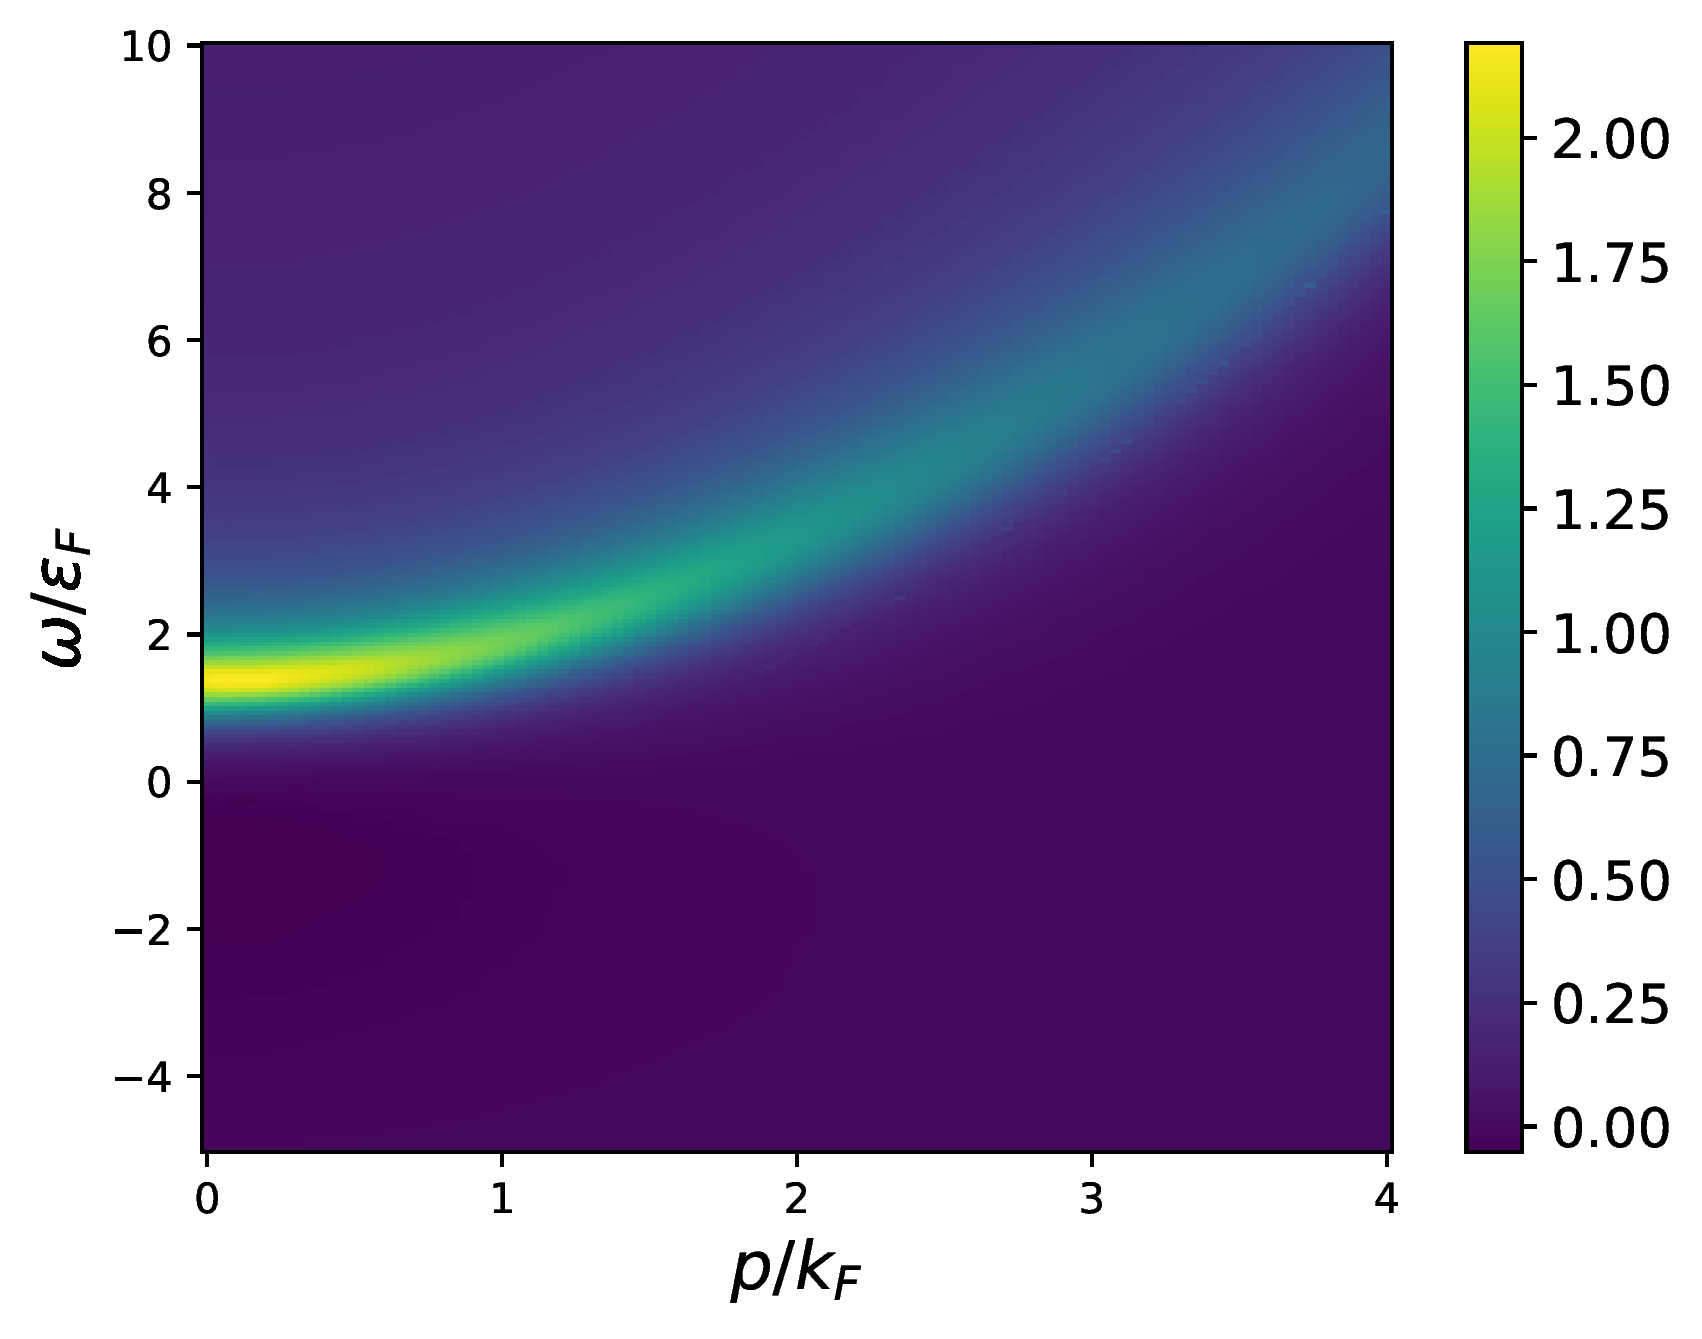
\includegraphics[width=0.328\textwidth]{figs/bos_spec_kFa=0.5.png}}
	\caption[Boson spectral function $\rho_{\phi}$ at different interaction strengths]{Results for the normalized bosonic dimer spectral function $h^2\rho_{\phi}\,\varepsilon_F/(8\pi)$ for $\beta\mu=0.13146$ at different interaction strengths $(k_Fa)^{-1}$ which correspond to (a) BCS regime (b) unitarity (c) BEC regime.}
	\label{fig:boson-specs}
\end{figure*}

Let us begin with the final results for the full momentum-dependent spectral functions at different interaction strengths. Fig.~\ref{fig:fermion-specs} shows results for the fermion spectral function $\rho_{\psi}$ and Fig.~\ref{fig:boson-specs} shows the corresponding bosonic dimer spectral functions $\rho_{\phi}$. In our unit system introduced in Chapter~\ref{chapter:introduction}, the frequency $\omega$ and momentum $p$ are measured in $\varepsilon_F$ and $k_F$, respectively, and the spectral functions have units of $\varepsilon^{-1}_F$. We state all results in dimensionless form. Note that the bosonic dimer spectral function is not normalized and depends on the choice of the Feshbach coupling $h$. In this way, it can be regarded as a pure interaction exchange boson and not a real particle. To eliminate the $h$-dependence, we multiply $\rho_{\phi}$ by $h^2/(8\pi)$ since $h^2G_{\phi}/(8\pi)$ is the relevant quantity which is related to the scattering amplitude, see Appendix~\ref{app:renormalization}.

The results for the bosonic dimer spectral function encode important information about the physics of the ultracold Fermi gas. First, we see a very broad peak structure for attractive interactions in the BCS regime, and a very sharp peak structure for repulsive interactions in BEC regime. This refers to the physical interpretation of condensed bosons on the BEC side. On this side of the BCS-BEC phase diagram, at $1/(k_Fa)=0.5$, the boson spectral function is very sharp and the system can be described as normal Bose liquid. On the BCS side of the crossover, at $1/(k_Fa)=-0.5$, the fermion spectral function is sharper and the system is described by a normal Fermi liquid, see Fig.~\ref{fig:crossover-phase-diagram}.

Fig.~\ref{fig:spec-convergence} shows the convergence behavior of the fermionic spectral function at unitarity for different temperatures. One can see that the spectral function at higher temperature convergences much faster than the spectral function at lower temperature. At $T=1.0\,T_F$, convergence is reached already after 6-7 iterations while the spectral function at $T=0.3\,T_F$ still varies considerably. Note the slow alternating convergence of the peak. This has to do with the fact that the bosonic spectral function gets very sharp and sensitive at lower temperatures close to the critical point, which will be discussed later in this Section. Without special treatment, like fixing the position of the boson peak or updating the spectral functions only partially~\cite{Frank2018}, it takes around 20 iterations to fully converge at $T=0.3\,T_F$. 

The fully converged fermion spectral functions obtained in this work are compared to the Keldysh results of Johannes Lang~\cite{Lang2023} in Fig.~\ref{fig:spec-comparison}. We find remarkable agreement between the two real-time approaches. However, a small residual shift of the peak positions is noticeable, which may result from remaining numerical issues. Nevertheless, a reconstruction from imaginary-time calculations by J. Lang via the Maximum Entropy Method~\cite{Jarrell2012} shows that the resulting spectral functions depend highly on the primer and may vary significantly. Without any prior information, the reconstructions differ notably from the real-time results. On the contrary, with real-time spectral functions as primer, the reconstructions yield the same results confirming the real-time calculations~\cite{Lang2023}. This shows the importance of computations directly in real frequencies.


\begin{figure}[h]
	\centering
	\subfigure[$T=0.3\,T_F$]{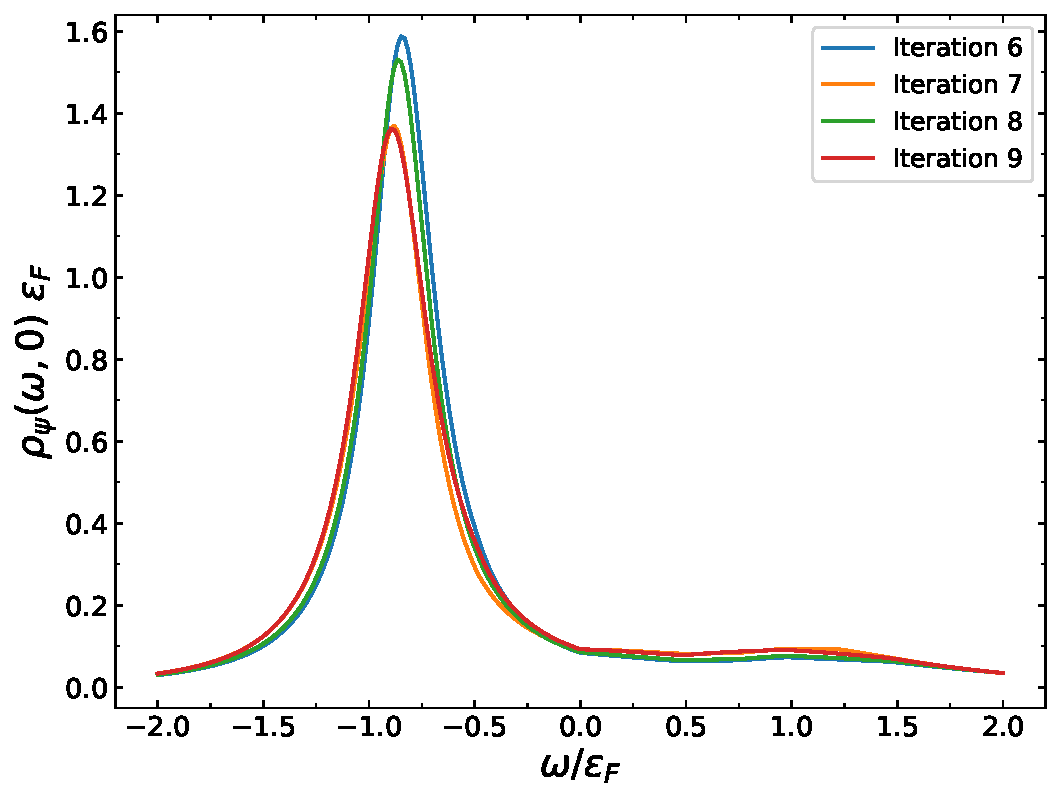
\includegraphics[width=0.47\textwidth]{figs/T=0.3_convergence.pdf}}
	\subfigure[$T=1.0\,T_F$]{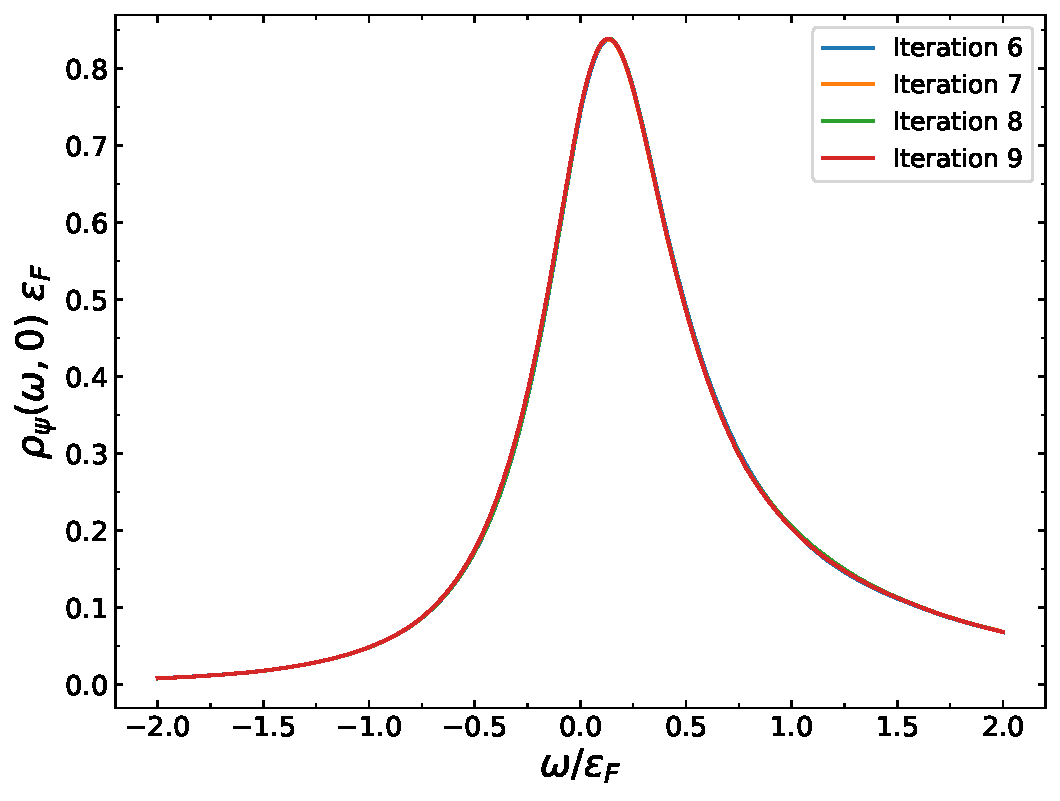
\includegraphics[width=0.47\textwidth]{figs/T=1_convergence.pdf}}
	\caption[Convergence of fermion spectral function at different temperatures]{Convergence of the fermionic spectral function at different temperatures.}
	\label{fig:spec-convergence}
\end{figure}


\begin{figure}[h]
	\centering
	\subfigure[$T=0.3\,T_F$]{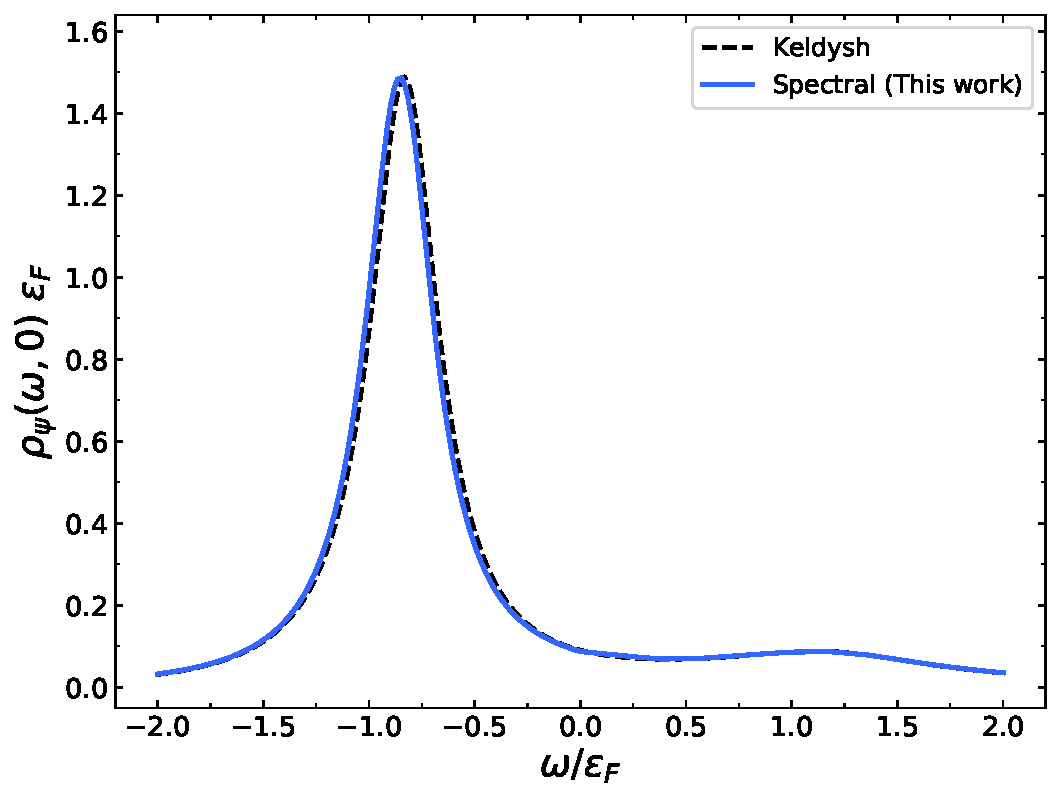
\includegraphics[width=0.47\textwidth]{figs/keldysh_comparison_T=0.3.pdf}}
	\subfigure[$T=1.0\,T_F$]{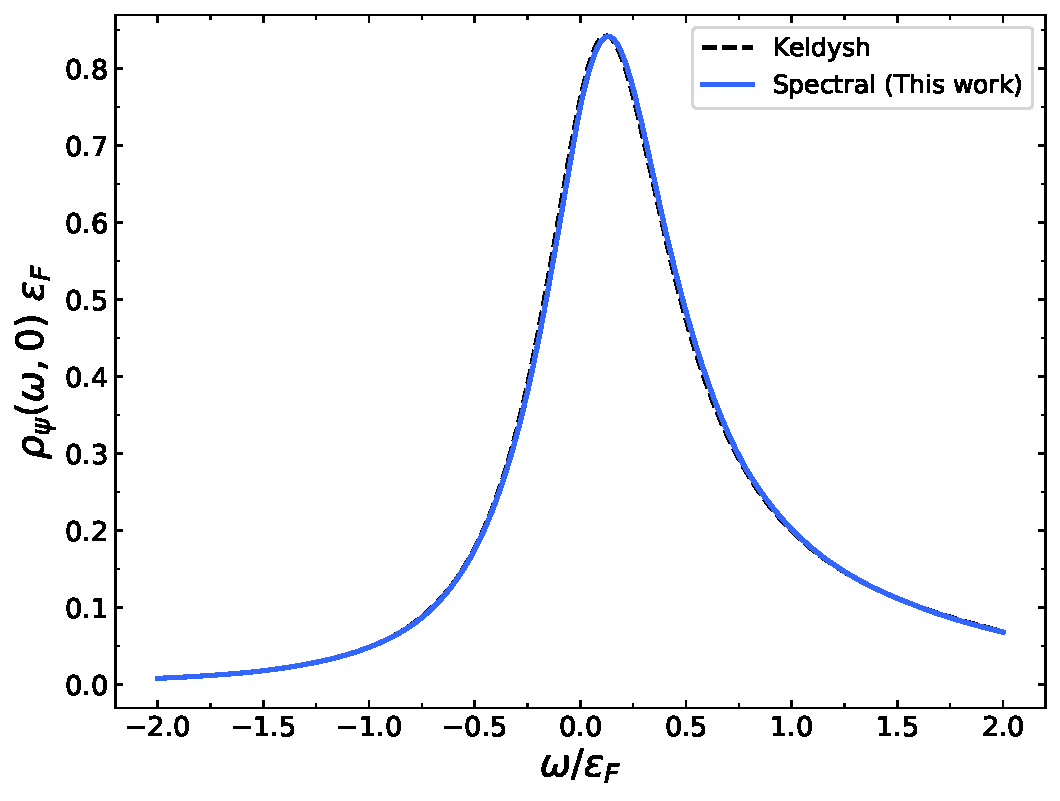
\includegraphics[width=0.47\textwidth]{figs/keldysh_comparison_T=1.pdf}}
	\caption[Comparison of spectral functions with the Keldysh approach]{Comparison of the fully converged fermionic spectral functions with a different real-time approach~\cite{Lang2023}, see explanations in the main text.}
	\label{fig:spec-comparison}
\end{figure}


Close to the critical temperature, the convergence behavior gets very problematic. Fig.~\ref{fig:fermion-specs-critical} and~\ref{fig:boson-specs-critical} show the fermion and boson spectral function for two consecutive iterations at $\beta\mu=2$. Similar to the oscillations in Fig.~\ref{fig:spec-convergence} at $T=0.3\,T_F$, we see the spectral functions alternating between two shapes, however, much more extreme. This situation can become very unstable and even increase in amplitude such that convergence is never reached. The reason for this is that the peak of the bosonic spectral function gets very sharp and sensitive at $\omega=0$ close to the critical temperature. Small numerical uncertainties in the fermion spectral function can lead to shifts of the bosonic peak below $\omega=0$, as can be seen in Fig.~\ref{fig:boson-specs-critical}. However, this situation is unphysical and numerically unstable, and leads to precondensed fermion spectral functions, see Fig.~\ref{fig:fermion-specs-critical}. In these cases, it is advisable to fix the boson peak at a certain value and then convert to the right interaction strength after convergence~\cite{Lang2023}. Another approach is to update the fermion spectral functions only partially to improve the convergence behavior~\cite{Frank2018}.

\begin{figure*}[t]
	\centering
	\subfigure[Iteration 7]{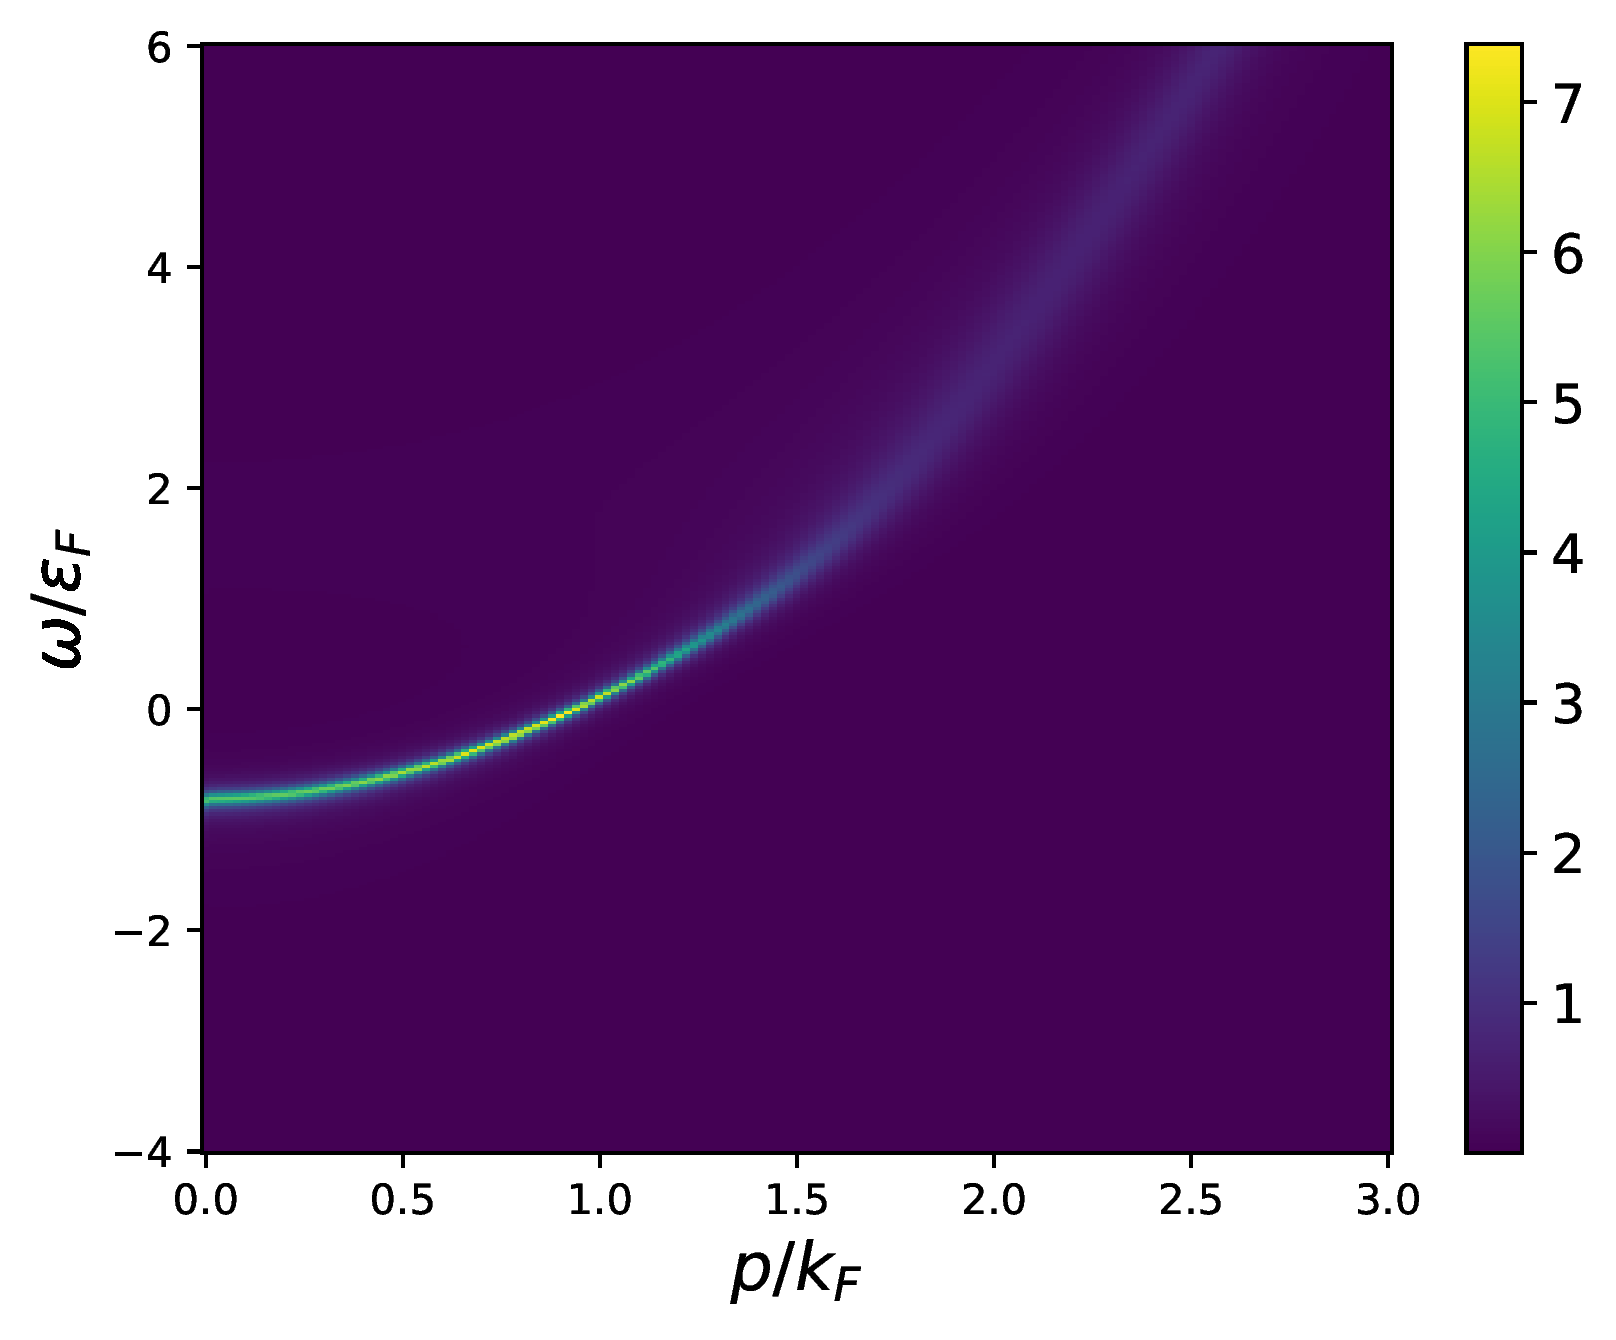
\includegraphics[width=0.39\textwidth]{figs/fermion_T=0.2_iter=7.png}}
	\subfigure[Iteration 8]{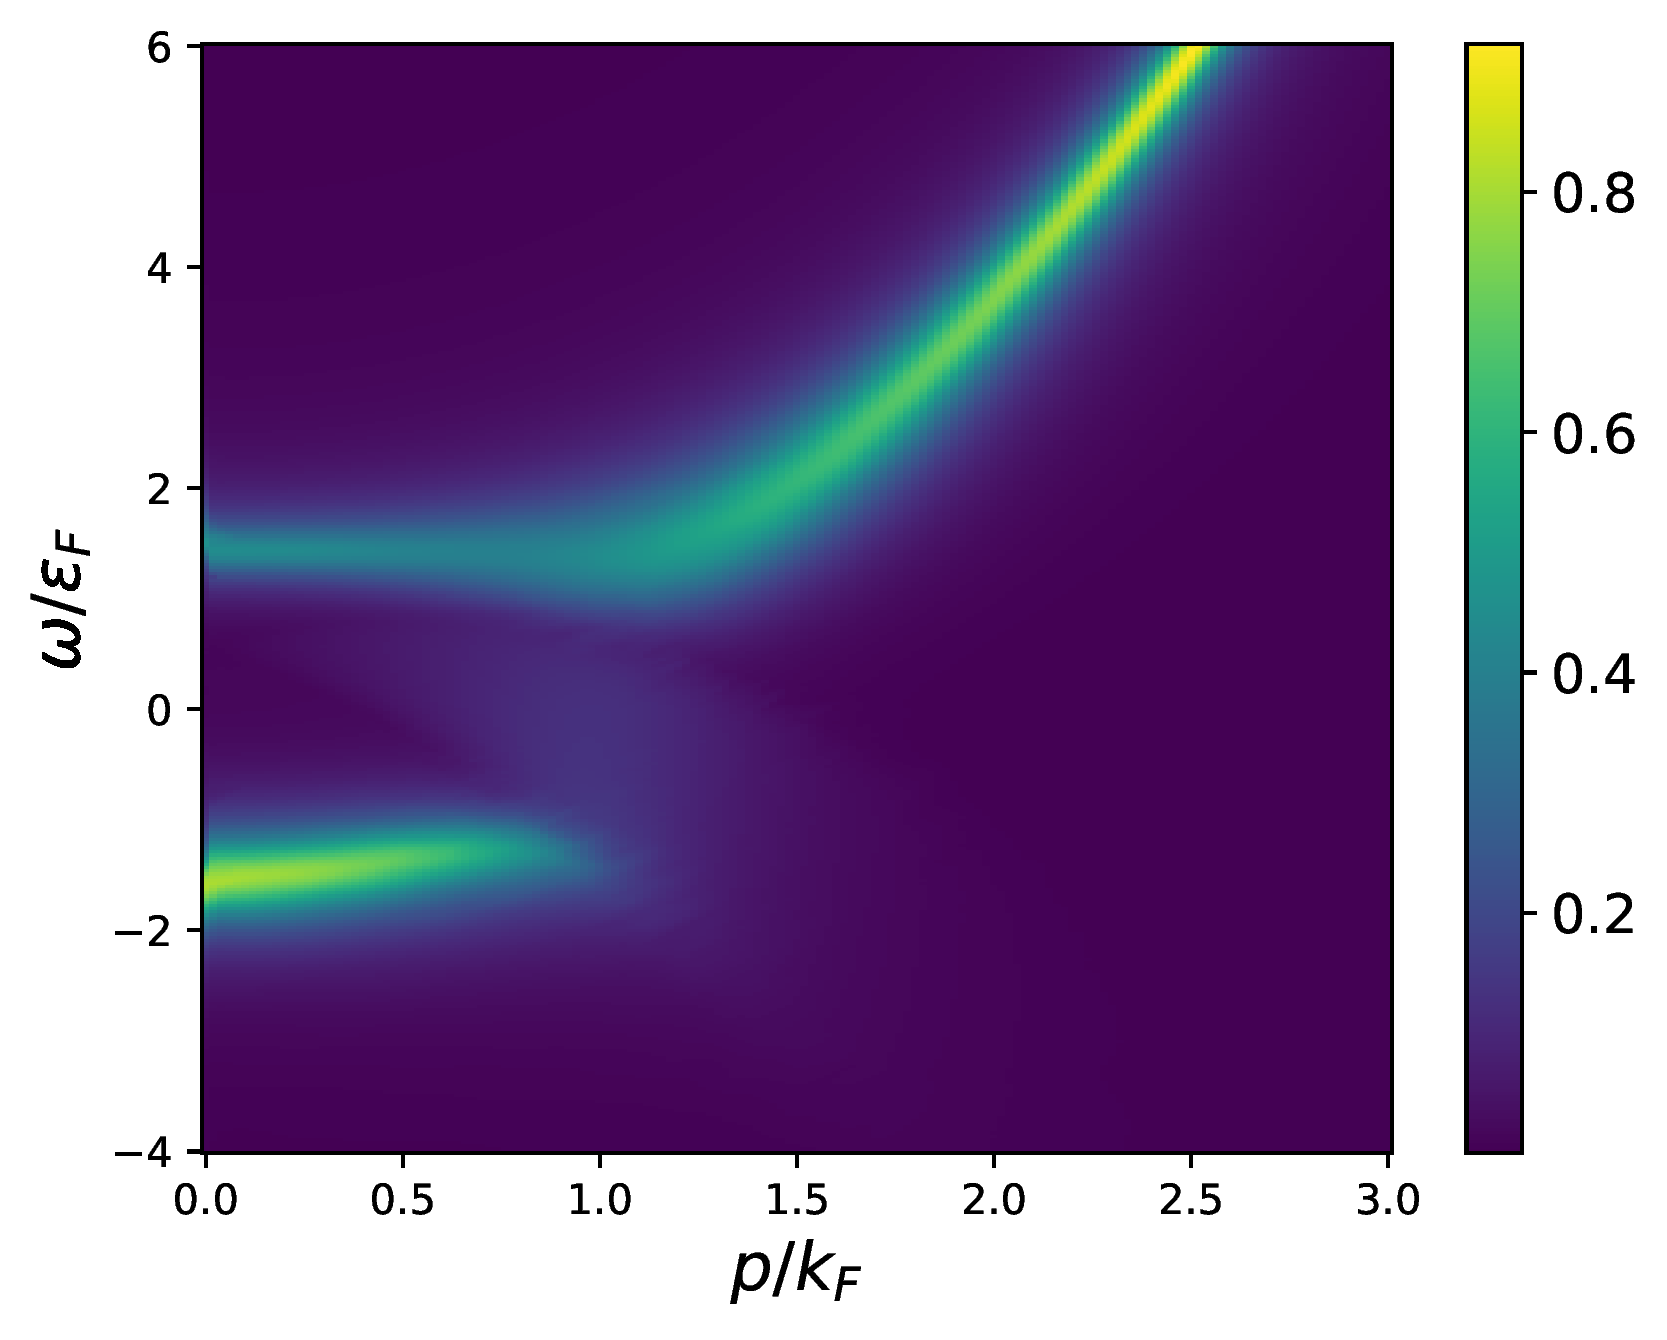
\includegraphics[width=0.401\textwidth]{figs/fermion_T=0.2_iter=8.png}}
	\caption[Fermion spectral functions close to the critical temperature]{Iterations of the fermionic spectral function $\rho_{\psi}\,\varepsilon_F$ at unitarity for $\beta\mu=2$.}
	\label{fig:fermion-specs-critical}
\end{figure*}
%
\begin{figure*}[t]
	\centering
	\subfigure[Iteration 7]{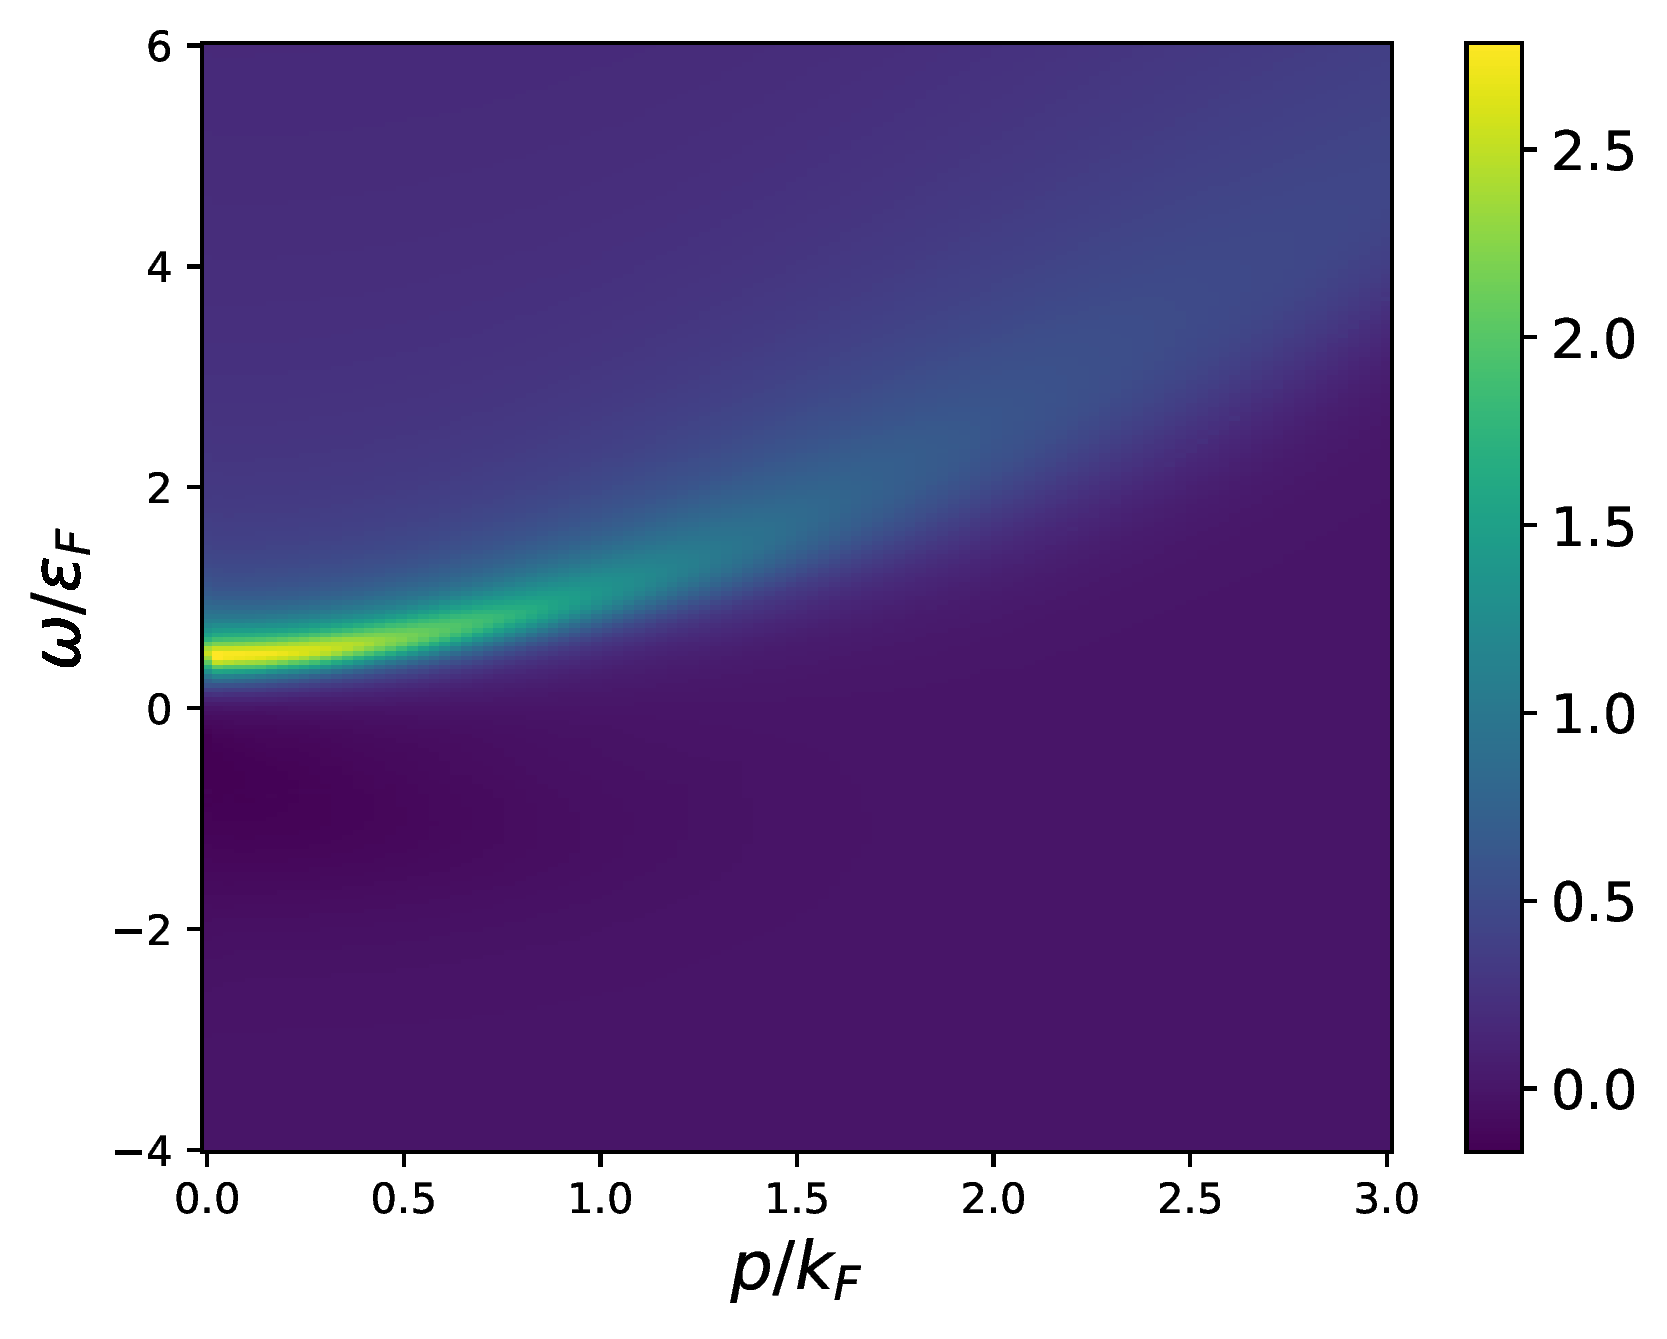
\includegraphics[width=0.392\textwidth]{figs/boson_T=0.2_iter=7.png}}
	\subfigure[Iteration 8]{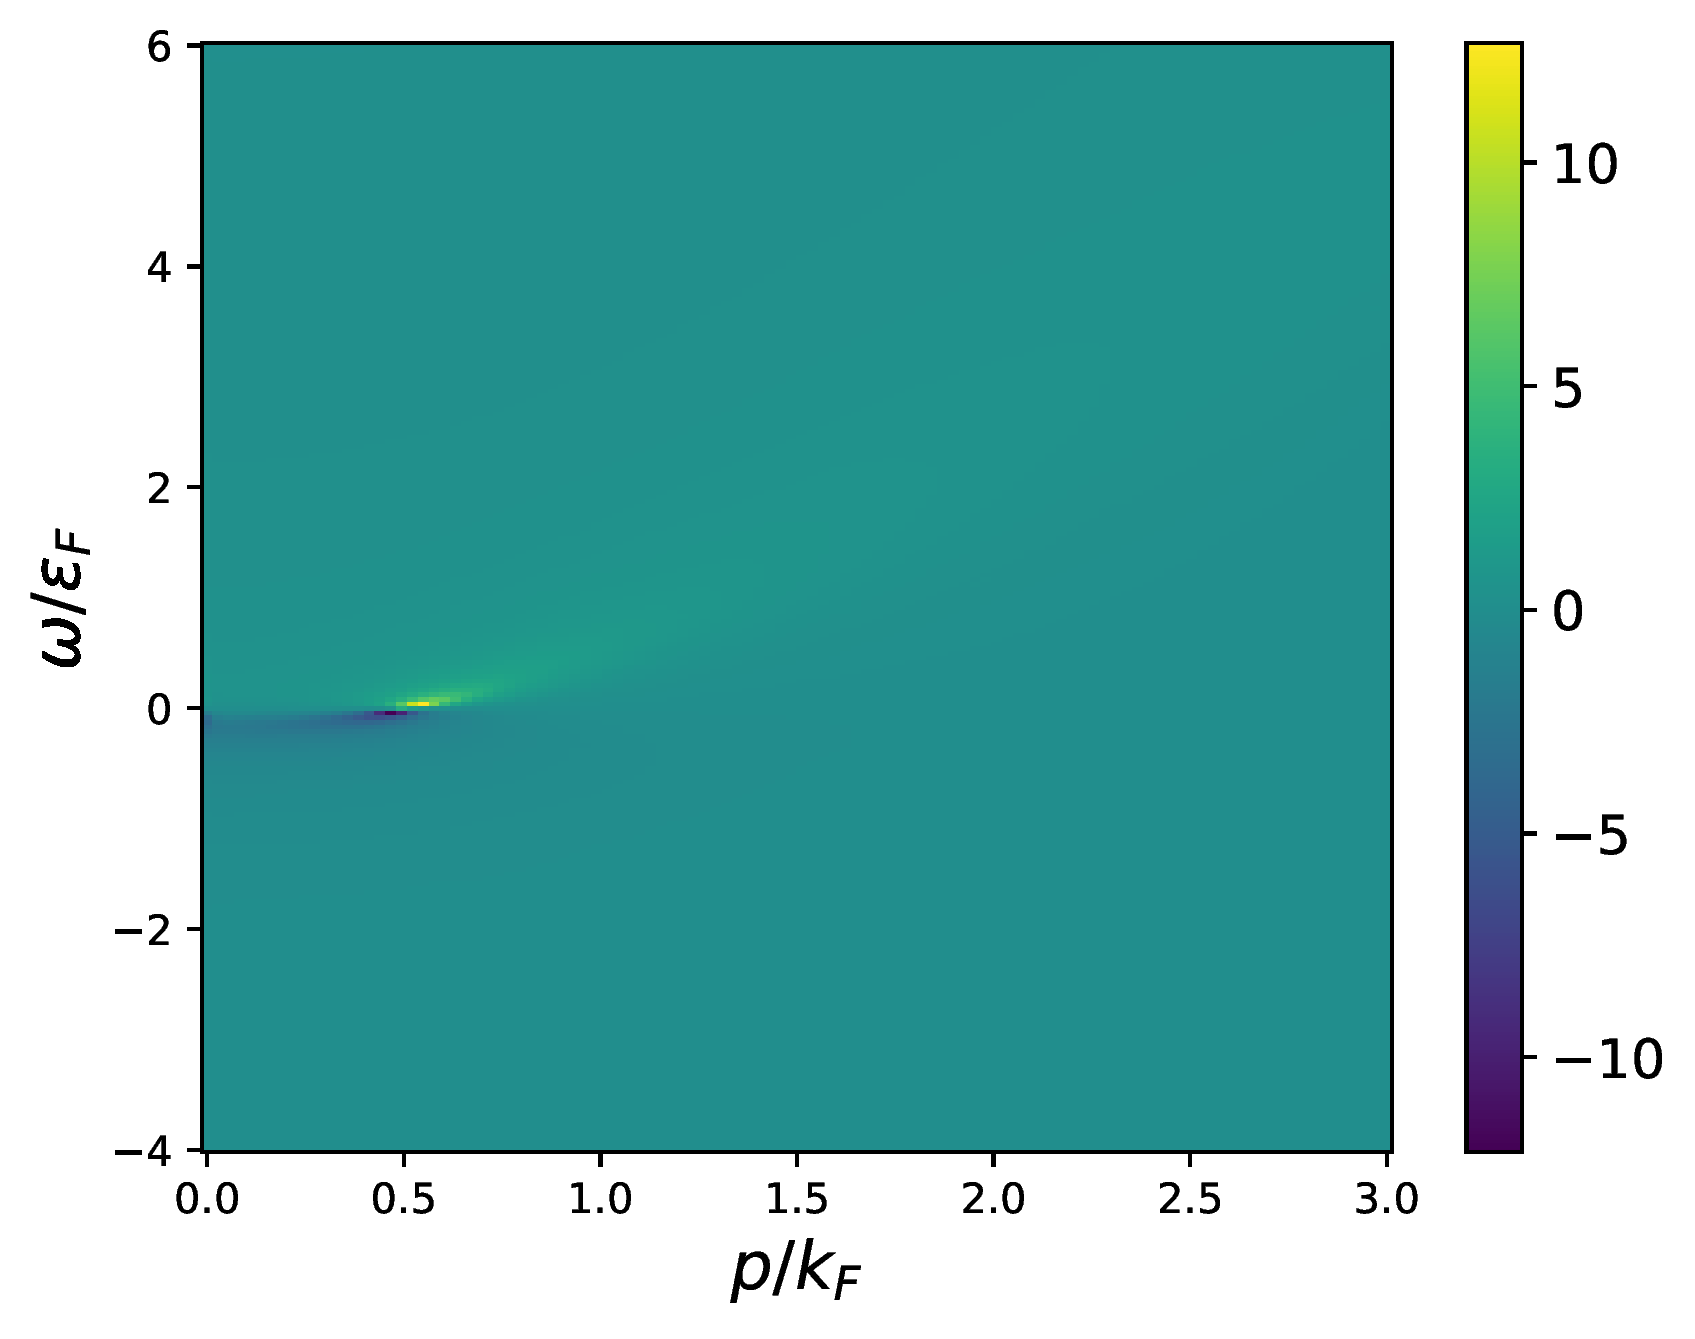
\includegraphics[width=0.397\textwidth]{figs/boson_T=0.2_iter=8.png}}
	\caption[Boson spectral functions close to the critical temperature]{Iterations of the bosonic dimer spectral function $h^2\rho_{\phi}\,\varepsilon_F/(8\pi)$ for $\beta\mu=2$.}
	\label{fig:boson-specs-critical}
\end{figure*}

As a consequence, the boson spectral function reveals crucial information about the critical region of the phase transition to the superfluid state. It is well-known that the onset of superfluidity is marked by the divergence of the boson propagator at zero frequency and momentum $G^{-1}_{\phi}(0,\bm{0})=0$. This property is known as the Thouless criterion~\cite{Thouless1960}. Thus, the closer and sharper the peak gets at the origin, the closer the system is to the phase transition, until the spectral function eventually diverges at the critical temperature.

\newpage

In order to evaluate spectral functions in the symmetry-broken phase, one has to ensure that the Thouless criterion~\cite{Thouless1960} is fulfilled, i.e. the bosons have to be gapless. At the same time, the gap parameter $\Delta$ has to be updated selfconsistently. This is a challenging numerical task and could not be implemented in the framework of this Thesis. There are many approaches and approximations to determine the gap parameter~\cite{Haussmann2009,Perali2004}. One way might be to choose $\Delta$ and a modified interaction strength such that the Thouless criterion is fulfilled~\cite{Haussmann2009,Lang2023}. Non-selfconsistent results in the broken phase can be obtained easily from the mean-field treatment presented in Section~\ref{section:nambu-gorkov-formalism}. The anomalous fermion spectral function is already well-known in the literature, see also~\cite{Bzdusek2013}. However, the bosonic anomalous spectral function is barely discussed. First non-selfconsistent considerations are presented in~\cite{Pieri2004-1}, however a selfconsistent treatment is absent and remains the subject for future work. We leave this as an exercise for the reader.

As an outlook for future work, one might also consider the mass and spin-imbalanced case, see~\cite{Punk2007,Punk2010,Frank2018}. In the following, we will use the spectral functions to calculate physical observables and benchmark our results against existing data.


\newpage


%%%%%%%%%%%%%%%%%%%%%%%%%%%%
\subsection*{Radio-frequency spectroscopy}
\label{section:rf-spectra}

From the calculated spectral functions, it is possible to obtain the experimentally measurable radio-frequency (rf) spectra~\cite{Punk2007,Schneider2009}. In this part, we apply our numerical framework at unitarity to describe the recent experimental data from MIT~\cite{Mukherjee2019}. For the computation of rf spectra $I(\omega)$ from the fermion spectral functions $\rho_{\psi}$, we take the formula~\cite{Haussmann2009}
%
\begin{align}
	\label{eq:rf-spectra}
	I(\omega) = \int_{\bm{q}} \rho_{\psi}(\varepsilon_{\bm{q}}-\omega-\mu,\bm{q})\, n_F(\varepsilon_{\bm{q}}-\omega-\mu) \,.
\end{align}
%
Note that the chemical potential $\mu(T)$ is temperature-dependent and has to be determined selfconsistently from the number equation~\eqref{eq:density}. More explicitly, the number density $n=1/(3\pi^2)$ is fixed by the choice $k_F=1$ and temperature is measured in units of $T_F$. Consequently, the chemical potential $\mu(T)$ has to be chosen such that the density stays constant~\cite{Tajima2019}. It is easy to see that the rf spectrum is normalized to the density $n$~\cite{Haussmann2009},
%
\begin{align}
	\label{eq:rf-dens}
	n = 2\int_{-\infty}^{\infty} d\lambda\, I(\lambda) \,.
\end{align}
%

\begin{figure}[htb]
	\begin{minipage}[t]{.492\textwidth}
		\centering
		\subfigure[]{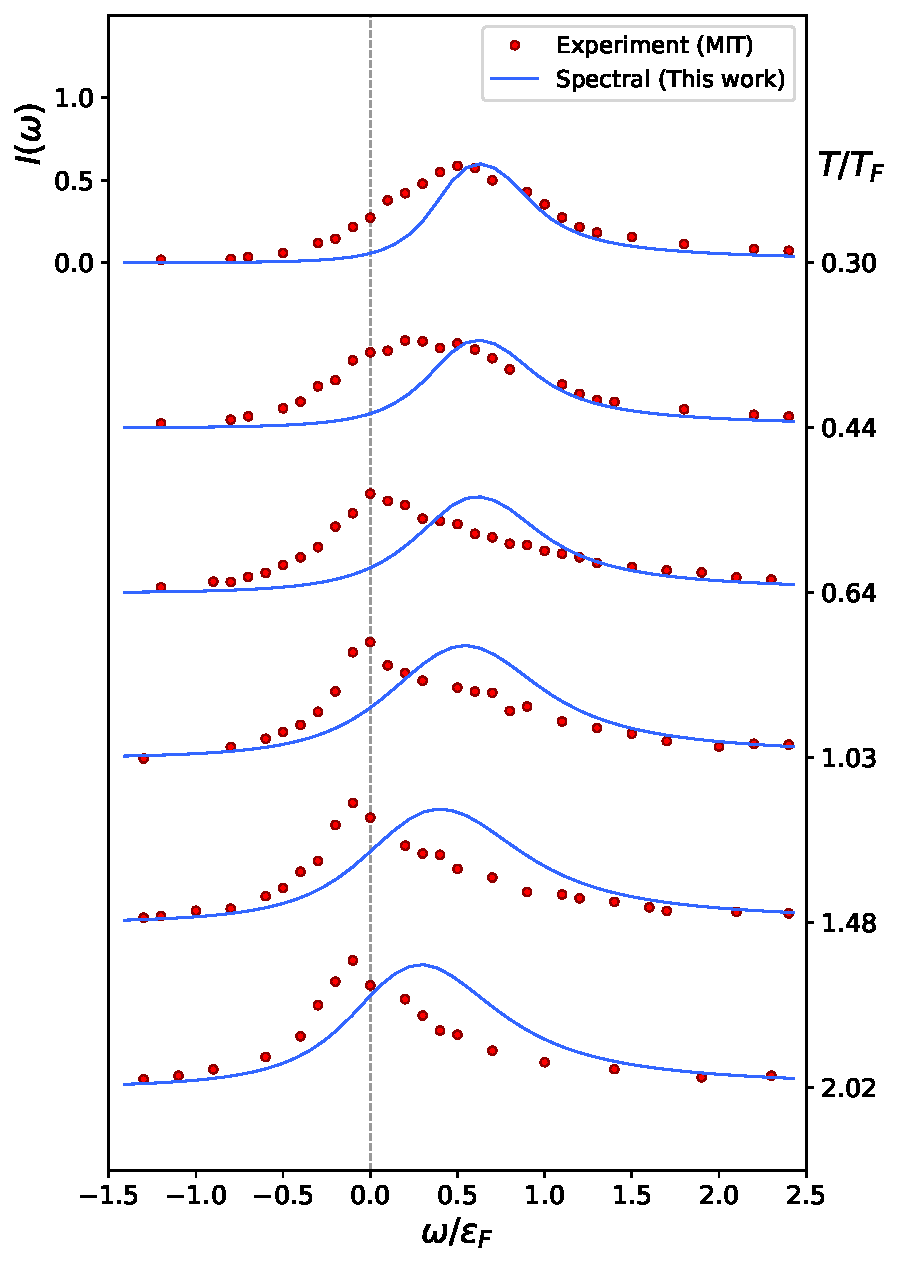
\includegraphics[width=\textwidth]{figs/rf_spectra.pdf}}
	\end{minipage}
	\hfill
	\begin{minipage}[t]{.49\textwidth}
		\centering
		\subfigure[]{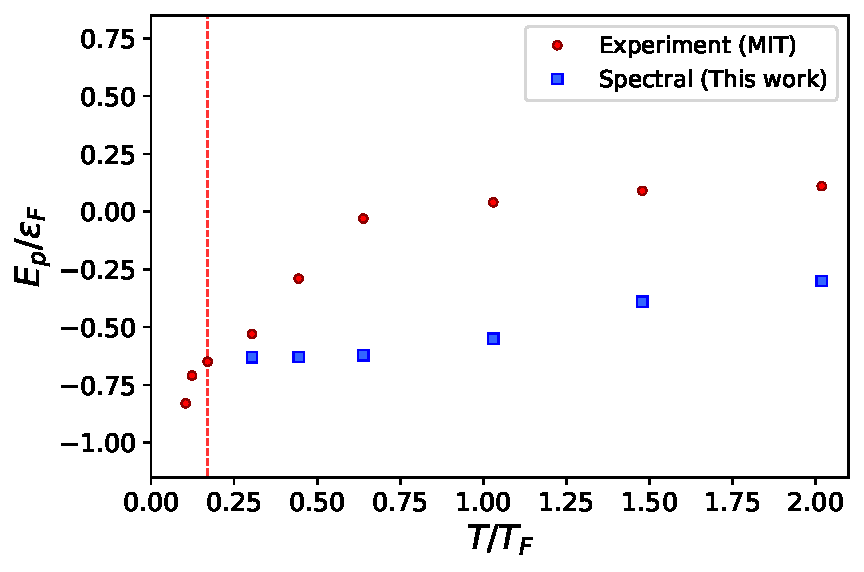
\includegraphics[width=0.95\textwidth]{figs/peak.pdf}}
		\raggedleft
		\subfigure[]{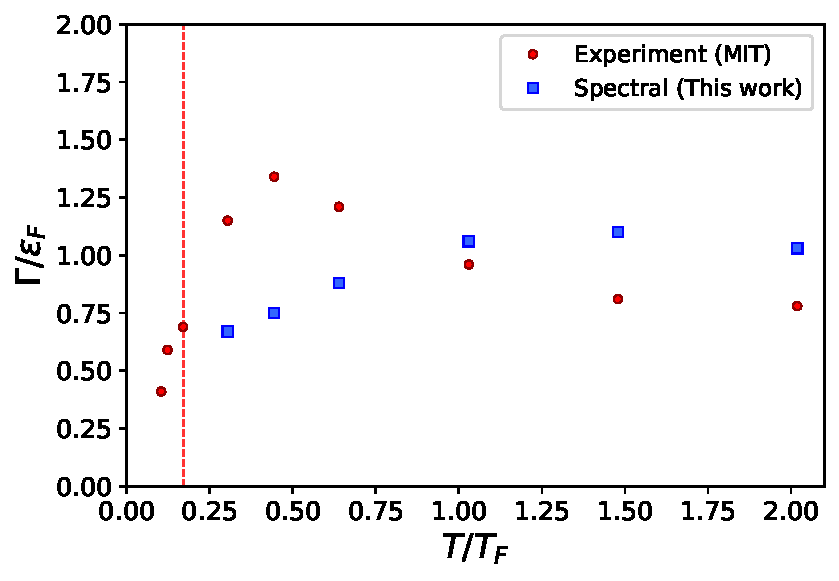
\includegraphics[width=0.92\textwidth]{figs/lifetime.pdf}}
	\end{minipage}
	\caption[Rf spectra of the unitary Fermi gas]{(a) Calculated ejection rf spectra $I(\omega)$ for the spin-balanced unitary Fermi gas as a function of the reduced temperature $T/T_F$. Results of this work (solid lines) are compared to experimental data from MIT~\cite{Mukherjee2019} (points). A Fourier broadening of $0.1\varepsilon_F$ to account for the finite experimental resolution, and a right-shift by $0.09\varepsilon_F$ to account for the final state interaction were applied. (b) Peak position ($E_p=-\hbar\omega$) and (c) full width at half maximum $\Gamma$ extracted from the rf spectra. The red vertical dashed line in (b) and (c) marks the superfluid phase transition.}
	\label{fig:rf-spectra}
\end{figure}

Fig.~\ref{fig:rf-spectra} shows our results in comparison with the experimental data from MIT~\cite{Mukherjee2019}. Apart from adjusting the peak heights, no fitting parameter have been used. In order to account for the finite rectangular rf pulse duration and, thus, a finite experimental resolution, the calculated spectra have to be convolved with $\mathrm{sinc}^2(\omega T/2)$, where $T$ is the rf pulse duration~\cite{Haussmann2009}. Additionally, the curves have to be right-shifted by an amount of $0.09\varepsilon_F$ to eliminate the residual final state effect~\cite{Hu2022}. Even after taking into account all these possible factors, the calculated rf spectra do not fit the experimental data for higher temperatures very well. This was also observed in~\cite{Hu2022} for the case of a highly spin-imbalanced unitary Fermi gas. A possible explanation might be the absence of a trap average, see e.g.~\cite{Schmidt2012}, since the trap potential is not ideally box shaped.


%%%%%%%%%%%%%%%%%%%%%%%%%%%%
\subsection*{Tan contact} \label{sec:contact}

Another test of the calculated spectral functions is the determination of the momentum-dependent occupation number $n(p)$ and Tans contact $C$~\cite{Rossi2018,Jensen2020}. The contact $C$ can be calculated in many different ways~\cite{Hu2011,Palestini2010}. One way is via the large frequency behavior of the rf spectrum $I(\omega)$~\cite{Haussmann2009,Schneider2009}
%
\begin{align}
	\label{eq:rf-contact}
	\lim_{\omega\rightarrow\infty} I(\omega) = \frac{C}{2\sqrt{2}\pi^2}\,\omega^{-3/2} \,.
\end{align}
%
Another direct way is via the imaginary-time boson propagator $G_{\phi}(\tau,\bm{x})$~\cite{Rossi2018}
%
\begin{align}
	\label{eq:vertex-contact}
	C = -G_{\phi}(\tau=0^-,\bm{x}=\bm{0}) \,,
\end{align}
%
which is used by imaginary-time computations like the Luttinger-Ward approach~\cite{Frank2018}. In this work, we extract the contact via the large momentum behavior of the occupation number $n(p)$~\cite{Boettcher2012, Hu2011}
%
\begin{align}
	\label{eq:contact}
	n(p) = \int_{\lambda} \rho_{\psi}(\lambda,\bm{p})\, n_F(\lambda) \,, \qquad \lim_{p\rightarrow\infty} n(p) = \frac{C}{p^4} \,.
\end{align}
%

\begin{figure}[h]
	\centering
	\subfigure[$\beta\mu=-0.5$]{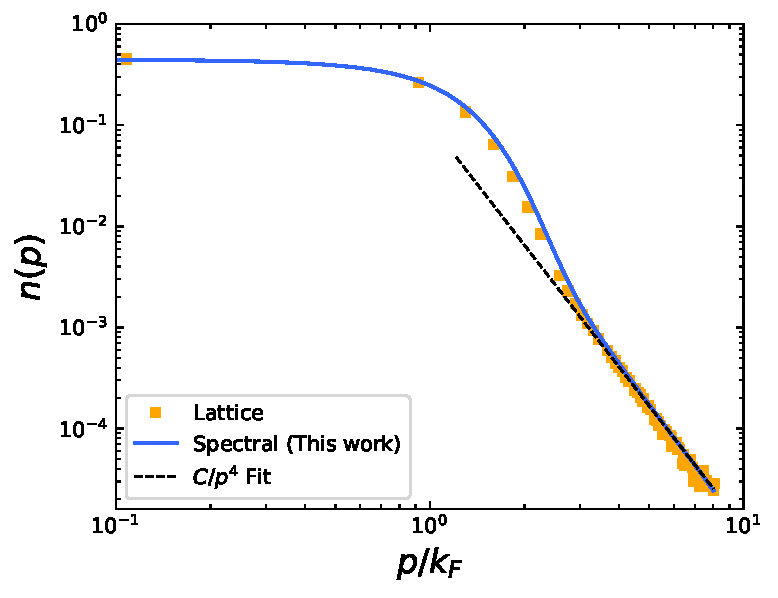
\includegraphics[width=0.47\textwidth]{figs/momentum_density_lattice_n05.pdf}}
	\subfigure[$\beta\mu=0.5$]{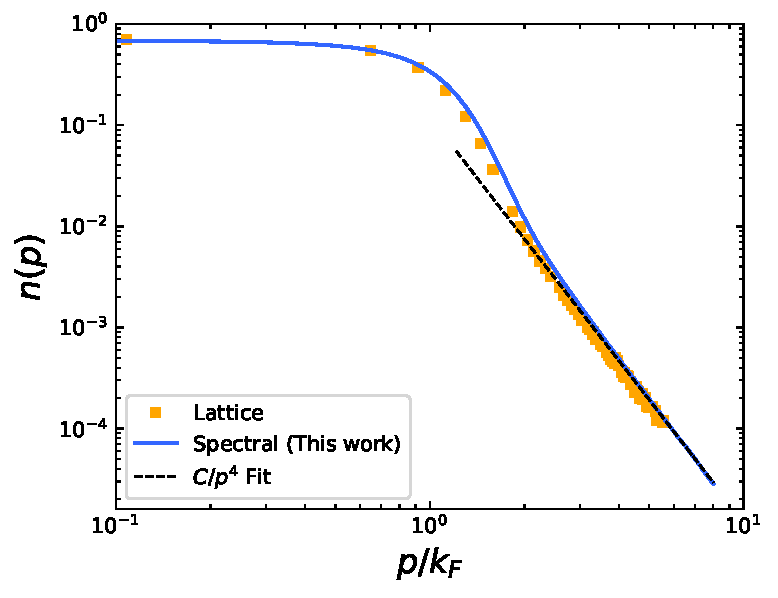
\includegraphics[width=0.47\textwidth]{figs/momentum_density_lattice_05.pdf}}
	\caption[Momentum distribution $n(p)$]{Large $p$ behavior of the occupation number $n(p)$. Results of this work are compared to lattice Monte Carlo data from~\cite{Bauer2023}.}
	\label{fig:momentum-density}
\end{figure}

\begin{figure}[t]
	\centering
	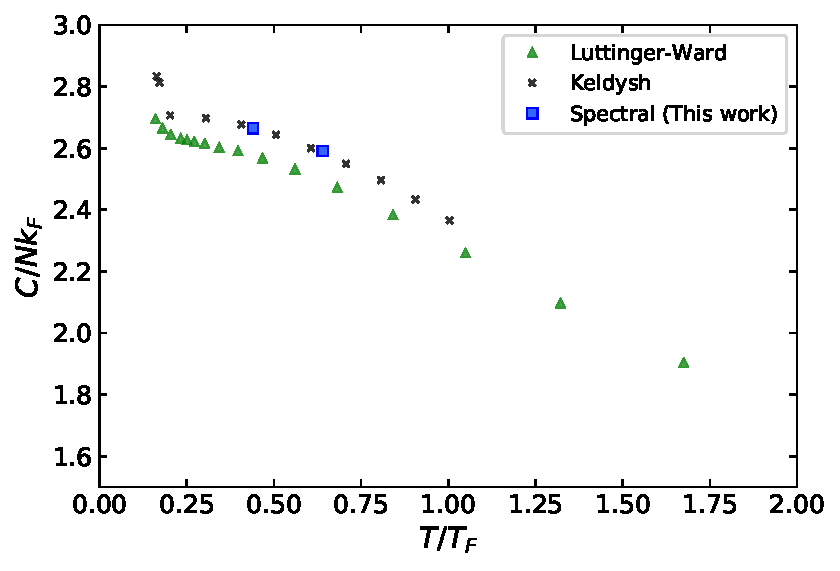
\includegraphics[width=0.67\linewidth]{figs/contact.pdf}
	\caption[Contact $C/Nk_F$ of the unitary Fermi gas]{Dimensionless contact $C/Nk_F$ of the spin-balanced unitary Fermi gas as a function of the reduced temperature $T/T_F$. Results of this work are compared to the Luttinger-Ward approach in imaginary-time~\cite{Frank2018} and another real-time approach using the Keldysh formalism~\cite{Lang2023}. The contact from the real-time approaches was obtained from the large momentum tail $n(k)=C/k^4$.}
	\label{fig:contact}
\end{figure}

Fig.~\ref{fig:contact} shows results for the Tan contact obtained with the spectral approach in comparison with the Luttinger-Ward~\cite{Frank2018} and Keldysh~\cite{Lang2023} approach. We note that the contact of the imaginary-time Luttinger-Ward method was determined directly from the boson propagator, while the contact of the real-time approaches was calculated from the large momentum behavior of the occupation number. Thus, these results are not directly comparable since the imaginary-time results are obtained with a different method. However, both real-time approaches seem to yield the same results.

Additionally, we show the momentum density distribution functions $n(p)$ in a double logarithmic plot for different $\beta\mu$ in Fig.~\ref{fig:momentum-density}. The $1/p^4$ tail for $p\gg k_F$ is clearly visible. We show lattice Monte Carlo results of Marc Bauer from our group for comparison. In the simulations, a lattice size of $13^3$ spatial points and 160 imaginary-time steps is used~\cite{Bauer2023}. In agreement with other works, the contact from selfconsistent T-matrix approaches seems to be slightly larger than experimental data or lattice Monte Carlo results~\cite{Mukherjee2019}. Thus, it is not surprising that the large momentum tail of our results is slightly above the lattice data.


%%%%%%%%%%%%%%%%%%%%%%%%%%%%
\subsection*{Density equation of state} \label{sec:density_eos}

The last benchmark of the calculated spectral functions is the density equation of state. Thermodynamic quantities, such as the total particle density, can be calculated precisely in Euclidean frequencies without the need of analytic continuation. For this reason, it is a good way to validate the new spectral approach against well tested and robust imaginary-time calculations. 

The total density $n$ of fermions at finite chemical potential $\mu$ and temperature $T$ can be calculated from the spectral function via~\cite{Schneider2009}
%
\begin{align} \label{eq:density}
	n = 2\,T\sum_{\omega_n}\int_{\bm{p}}G_{\psi}(\omega_n,\bm{p}) = 2\int_{\lambda,\bm{p}}\rho_{\psi}(\lambda,\bm{p})\,n_F(\lambda) \,.
\end{align}
%
Fig.~\ref{fig:density_eos} shows the results for the normalized density $n/n_0$ as a function of dimensionless chemical potential $\beta\mu$ in comparison with all other available approaches. The density $n_0$ of the non-interacting Fermi gas is given by $n_0=2\int_{\bm{p}}n_F(p^2-\mu)=-2\mathrm{Li}_{3/2}(-e^{\beta\mu})/\lambda_T^3$, where $\lambda_T=\sqrt{4\pi/T}$ is the thermal wavelength and $\mathrm{Li}_{3/2}$ is a polylogarithm function~\cite{Abramowitz1972}.

In the calculation of the density through the spectral function, the high momentum tail can not be neglected. If the numerical spectral function is given on a finite grid with momentum cutoff $\Lambda\gg k_F$, the contribution from outside the grid follows with~\eqref{eq:contact},
%
\begin{align}
	\delta n_{>\Lambda} = 2 \int_{\Lambda}^{\infty}\frac{d^3p}{(2\pi)^3} \frac{C}{p^4} = \frac{C}{\pi^2\Lambda} \,,
\end{align}
where $C$ is the contact introduced before. Note that this estimation is only valid when the numerical cutoff $\Lambda$ is chosen large enough, such that the asymptotic behavior set in already. Then one can extrapolate the large $p$ region and take its contribution into account. Fig.~\ref{fig:momentum-density} shows that our numerics reproduce the asymptotic $1/p^4$ tail very well for $p\approx 8k_F$ already. The missing contribution from the high momentum tail is around $10\%$.

It is important to note that our real-time method reproduces the results of the well tested Luttinger-Ward approach~\cite{Haussmann2007,Frank2018}. Moreover, the other real-time approach based on the Keldysh formalism agrees very well with our results. This agreement is crucial since all methods build on the same underlying theory and resummation of diagrams.


\begin{figure}[t]
	\centering
	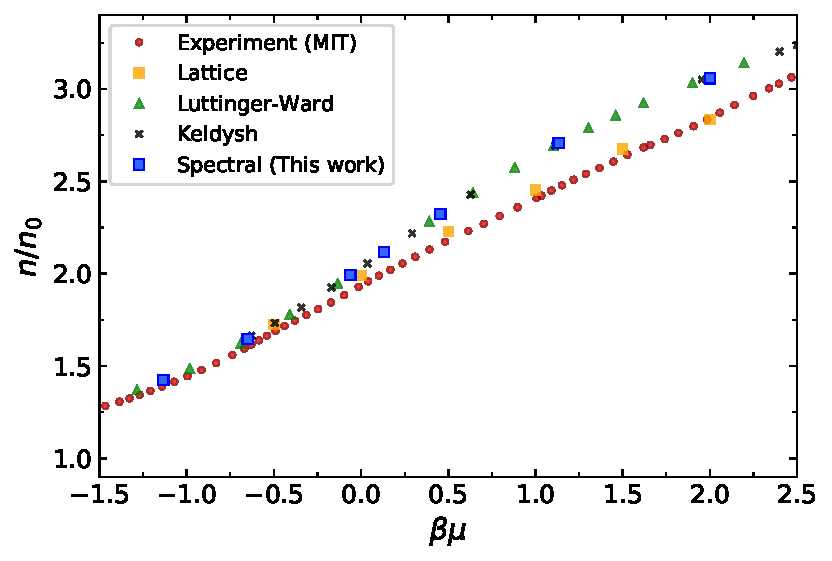
\includegraphics[width=0.67\linewidth]{figs/density_eos.pdf}
	\caption[Density equation of state of the unitary Fermi gas]{Normalized density $n/n_0$ of the spin-balanced unitary Fermi gas as a function of dimensionless chemical potential $\beta\mu$. Results directly obtained in real frequencies (this work) in comparison with experimental data from MIT~\cite{Ku2012}, lattice Monte Carlo data from~\cite{Bauer2023}, Luttinger-Ward results~\cite{Haussmann2007} and another real-time approach based on the Keldysh formalism~\cite{Lang2023}.}
	\label{fig:density_eos}
\end{figure}

	\chapter{Fermi Polaron}
\label{chapter:fermi-polaron}

In this Chapter, we consider the extremely spin-imbalanced case in which there is only one spin-$\downarrow$ impurity inside a Fermi sea of spin-$\uparrow$ particles. This scenario is well-known as the Fermi polaron problem and has been studied extensively in vacuum~\cite{Schmidt2011,Kamikado2017}. However, spectral properties at finite temperature were just recently investigated by Hu et al.~\cite{Hu2022} with a non-selfconsistent approach. In the following, we apply our fully selfconsistent real-time framework to study the spectral and quasiparticle properties of the Fermi polaron at finite temperature.

\section{Theoretical description}
\label{section:polaron-theoretical-description}

In this Section, we introduce the general theoretical description of a single impurity immersed in a Fermi sea of particles with different spin and derive the selfconsistent equations. The general microscopic action which accounts for spin and mass imbalance is given by
%
\begin{align}
	\label{eq:polaron-action}
    S[\psi, \phi] = \int_{\tau,\bm{x}}\,
    \Big[ \sum_{\sigma=\uparrow,\downarrow} \psi^*_{\sigma} (\partial_{\tau} - \nabla^2/(2m_{\sigma}) - \mu_{\sigma}) \psi_{\sigma}
    + \nu \phi^* \phi - h (\phi^* \psi_{\uparrow} \psi_{\downarrow} - \phi \psi^*_{\uparrow} \psi^*_{\downarrow}) \Big] \,,
\end{align}
%
where $2m_{\uparrow} = 1$ and $\mu_{\uparrow}$ is the mass and chemical potential of the majority atoms, and $2m_{\downarrow} = (1+\alpha)/(1-\alpha)$ and $\mu_{\downarrow}\leq 0$ is for the impurity. The mass imbalance $\alpha$ is connected to the reduced mass $2m_r = (1+\alpha)/2$ and satisfies $-1 < \alpha = (m_{\downarrow}-m_{\uparrow})/(m_{\downarrow}+m_{\uparrow}) < 1$.

The selfconsistent equations for the Fermi polaron problem can be derived by the same means as described in Chapter~\ref{chapter:bcs-bec-crossover}, however, some simplifications can be made. First of all, we can replace again all three-point functions by the classical vertices $\Gamma^{(3)}=S^{(3)}$. Moreover, since there is only one impurity in the system, the majority atoms are barely affected and can be treated as non-interacting particles. The simplified Dyson-Schwinger equations for the Fermi polaron problem are shown diagrammatically in Fig.~\ref{fig:polaron_DSEs} and will be discussed in the following. It is well-known that the strong spin-imbalance hinders the system to form a condensate, such that the physics is described completely by the normal phase~\cite{Punk2010}. However, there is still a non-trivial polaron-to-molecule phase transition~\cite{Schmidt2013}.

As pointed out before, the spin-$\uparrow$ majority atoms in the Fermi sea are not dressed and can be described by the classical fermion Green's function
%
\begin{align}
	\label{eq:maj}
    G^{(0)}_{\uparrow}(\omega_n, \bm{p})
    = \frac{1}{-i\omega_n+\varepsilon_{\bm{p}}-\mu_{\uparrow}} \,.
\end{align}
%
where $\varepsilon_{\bm{p}}=\bm{p}^2/(2m_{\uparrow})=\bm{p}^2$ is the majority dispersion relation. However, the impurity Green's function obtains a self-energy and can be written as (see Eq.~\eqref{eq:selfconsistent-equations})
%
\begin{align}
	\label{eq:min}
    G_{\downarrow}(\omega_n, \bm{p})
    = \frac{1}{-i\omega_n+\varepsilon^{(I)}_{\bm{p}}-\mu_{\downarrow}
    -\Sigma(\omega_n, \bm{p})} \,,
\end{align}
%
where $\varepsilon^{(I)}_{\bm{p}}=\bm{p}^2/(2m_{\downarrow}) = \bm{p}^2\,(1-\alpha)/(1+\alpha)$ is the impurity dispersion relation~\cite{Hu2022}.

\begin{figure}[t]
	\begin{center}
		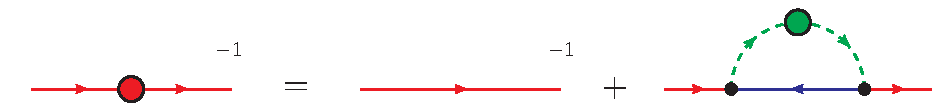
\includegraphics[width=0.8\textwidth]{figs/polaron_prop_DSE.pdf} \\
		\vspace{0.5cm}
		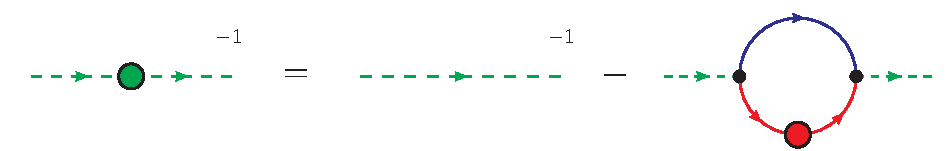
\includegraphics[width=0.8\textwidth]{figs/polaron_boson_DSE.pdf} 
	\end{center}
	\caption[Polaron Dyson-Schwinger equations]{Simplified Dyson-Schwinger equations for the Fermi polaron. The blue propagator of the Fermi sea is just the classical fermion propagator and only the red polaron Greens function gets dressed. All vertices are classical.}
	\label{fig:polaron_DSEs}
\end{figure}

The impurity self-energy $\Sigma(\omega_n, \bm{p})$ is given by (see Fig.~\ref{fig:polaron_DSEs})
%
\begin{align}
	\label{eq:self}
    \Sigma(\omega_n, \bm{p})
    = h^2 \int\frac{d^{3}q}{(2\pi)^{3}}\, T\sum_{\Omega_m}
    G_{\phi}(\Omega_m, \bm{q})
    G^{(0)}_{\uparrow}(\Omega_m-\omega_n, \bm{q-p}) \,.
\end{align}
%
And the molecule propagator $G_{\phi}(\omega_m, \bm{q})$ satisfies again the relation~\eqref{eq:selfconsistent-equations}
%
\begin{align}
	\label{eq:mol}
    G^{-1}_{\phi}(\omega_m, \bm{q}) = -\frac{h^2}{8\pi a} - \Pi(\omega_n,\bm{p}) \,,
\end{align}
%
with the molecule self-energy $\Pi(\omega_n,\bm{p})$ given by
%
\begin{align}
	\label{eq:pol}
    \Pi(\omega_n, \bm{p}) =
    h^2 \int\frac{d^{3}q}{(2\pi)^{3}}\left[ T\sum_{\Omega_m} G_{\downarrow}(\Omega_m, \bm{q}) G^{(0)}_{\uparrow}(\omega_n-\Omega_m, \bm{p-q}) - \frac{1+\alpha}{2\bm{q}^2} \right] \,,
\end{align}
%
where the counterterm changed because of the mass-imbalance~\cite{Hu2022}.

Again, these coupled equations can be solved selfconsistently in real frequencies with the spectral representation. Analytical continuation $i\omega_n = \omega + i0^+$ to the retarded self-energies and taking the imaginary part yields (see Eq.~\eqref{eq:imaginary-part-self-energies})
%
\begin{align}
	\label{eq:imaginary-part-polaron-self-energies}
	\mathrm{Im}\,\Sigma^R(\omega,\bm{p}) &= -\pi h^2\int_{\bm{q}}
	\rho_{\phi}(\omega+\varepsilon_{\bm{q-p}}-\mu_{\uparrow},\bm{q})
	\,n_F(\varepsilon_{\bm{q-p}}-\mu_{\uparrow}) \,, \notag \\
	\mathrm{Im}\,\Pi^R(\omega,\bm{p}) &= \pi h^2\int_{\bm{q}}
	\rho_{\downarrow}(\omega-\varepsilon_{\bm{p-q}}+\mu_{\uparrow},\bm{q})
	\left[1-n_F(\varepsilon_{\bm{p-q}}-\mu_{\uparrow})\right] \,.
\end{align}
%
Here, we used the fact that the quantum statistics of the impurity is not relevant and the molecule occupation number is vanishingly small in the single-impurity limit~\cite{Hu2022}. For a finite impurity concentration, one has to be a bit more careful, see~\cite{Hu2018,Tajima2019}. Additionally, we are left with only 2-dimensional integrals since the majority is non-interacting and the spectral parameter can be integrated out.

From here, the real part can be obtained again via the Kramers-Kronig relation~\eqref{eq:kramers-kronig} and all the numerical steps stay the same. For the boson self-energy, the same subtraction schemes can be used. We refer the reader to Appendix~\ref{app:boson-self-energy-calculation} and~\ref{app:numerical-implementation} for more details on the analytical results and numerical implementation.


\section{Results}
\label{section:polaron-results}

The Fermi polaron problem has been studied intensively in previous works. First excitation spectra at zero temperature were obtained by R. Schmidt and T. Enss using fRG and Padé approximation methods in~\cite{Schmidt2011}. Their results were confirmed and generalized with the fRG in real frequencies by K. Kamikado et al. in~\cite{Kamikado2017}. Since then a numerous amount of articles concerning the quasiparticle properties of the 3-dimensional Fermi polaron have been published~\cite{Mulkerin2019,Scazza2022,Veillette2008,Vlietinck2013}. Also spin-imbalanced gases in general have been investigated with different methods~\cite{Chevy2006,Prokofev2008,VanHoucke2020,Veillette2008}. Recently, also 2-dimensional Fermi gases~\cite{Schmidt2012,Bauer2014,Mulkerin2015}, Bose polarons~\cite{Tajima2021} and general Bose-Fermi mixtures~\cite{Milczewski2022} have been studied.

With the spectral approach described above, we can obtain spectral functions at arbitrary temperatures and mass-imbalances. In this part, we will show the equivalence to previous works for the mass-balanced case and discuss possible generalizations. In the end, selfconsistent and non-selfconsistent results for the rf spectra of the unitary Fermi polaron are presented and compared to recent works~\cite{Tajima2019,Hu2008,Yan2019}. 

Let us begin with a general discussion of the results at zero temperature. These are obtained by replacing $n_F(x)\rightarrow\theta(-x)$, as mentioned in Section~\ref{section:normal-phase}, and using the vacuum boson self-energy. Fig.~\ref{fig:specs-comparison} shows the selfconsistent polaron spectral functions at $T=0$ for different interaction strengths. These results agree well with the ones obtained in~\cite{Schmidt2011,Kamikado2017} using the fRG. For the polaron ground state energy at unitarity, we obtain $\mu_{\downarrow}\simeq-0.62$ which compares favorably with~\cite{Combescot2008}. The non-selfconsistent result is $\mu_{\downarrow}\simeq-0.61$ and shows the equivalence to Chevy's variational  ansatz~\cite{Chevy2006,Combescot2007}. In vacuum, the chemical potential of the non-interacting Fermi sea is $\mu_{\uparrow}=1$. Contrary to the spin-balanced case, the Padé approximation method from~\cite{Schmidt2011} is quite reasonable in the polaron case. This might stem from the fact that the majority particles are not dressed and the structure of the polaron spectral function is simpler. However, only real-time approaches, like in~\cite{Kamikado2017} or this work, can compute fully correct spectral functions.

\begin{figure}[b]
	\centering
	\subfigure[$(k_Fa)^{-1} = -0.5$]{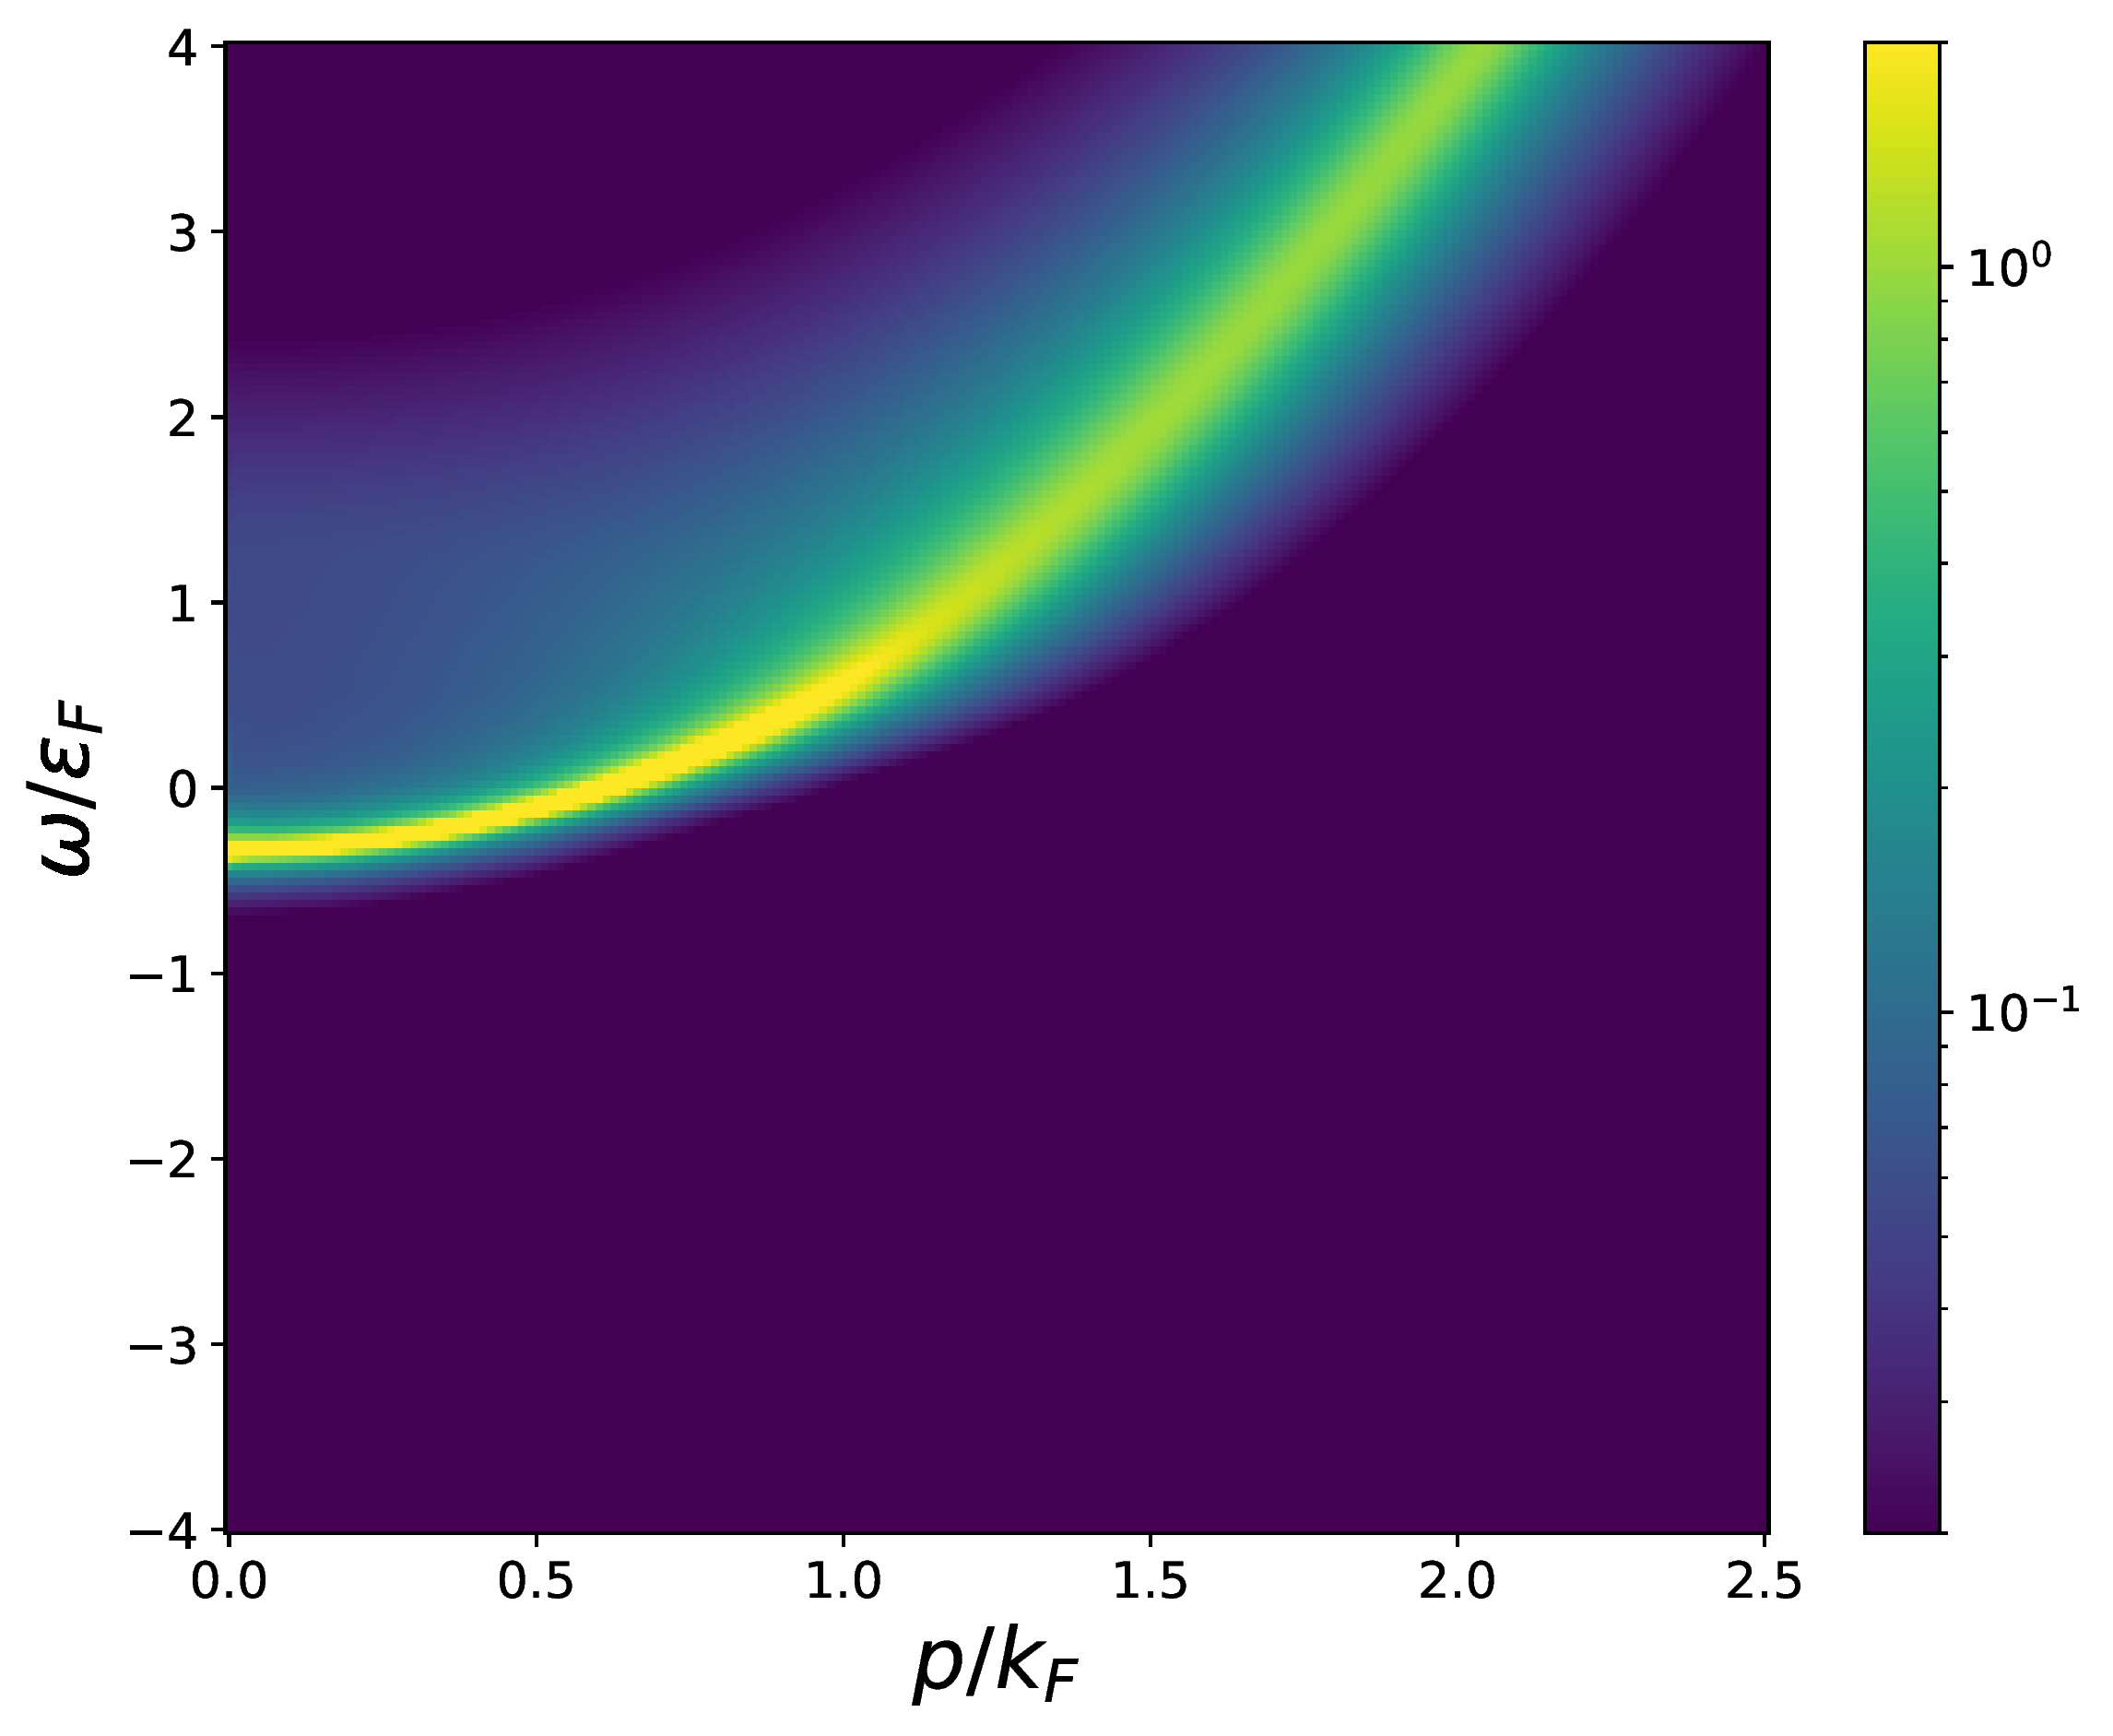
\includegraphics[width=0.24\textwidth]{figs/polaron_n05kfa.png}} 
	\subfigure[$(k_Fa)^{-1} = 0$]{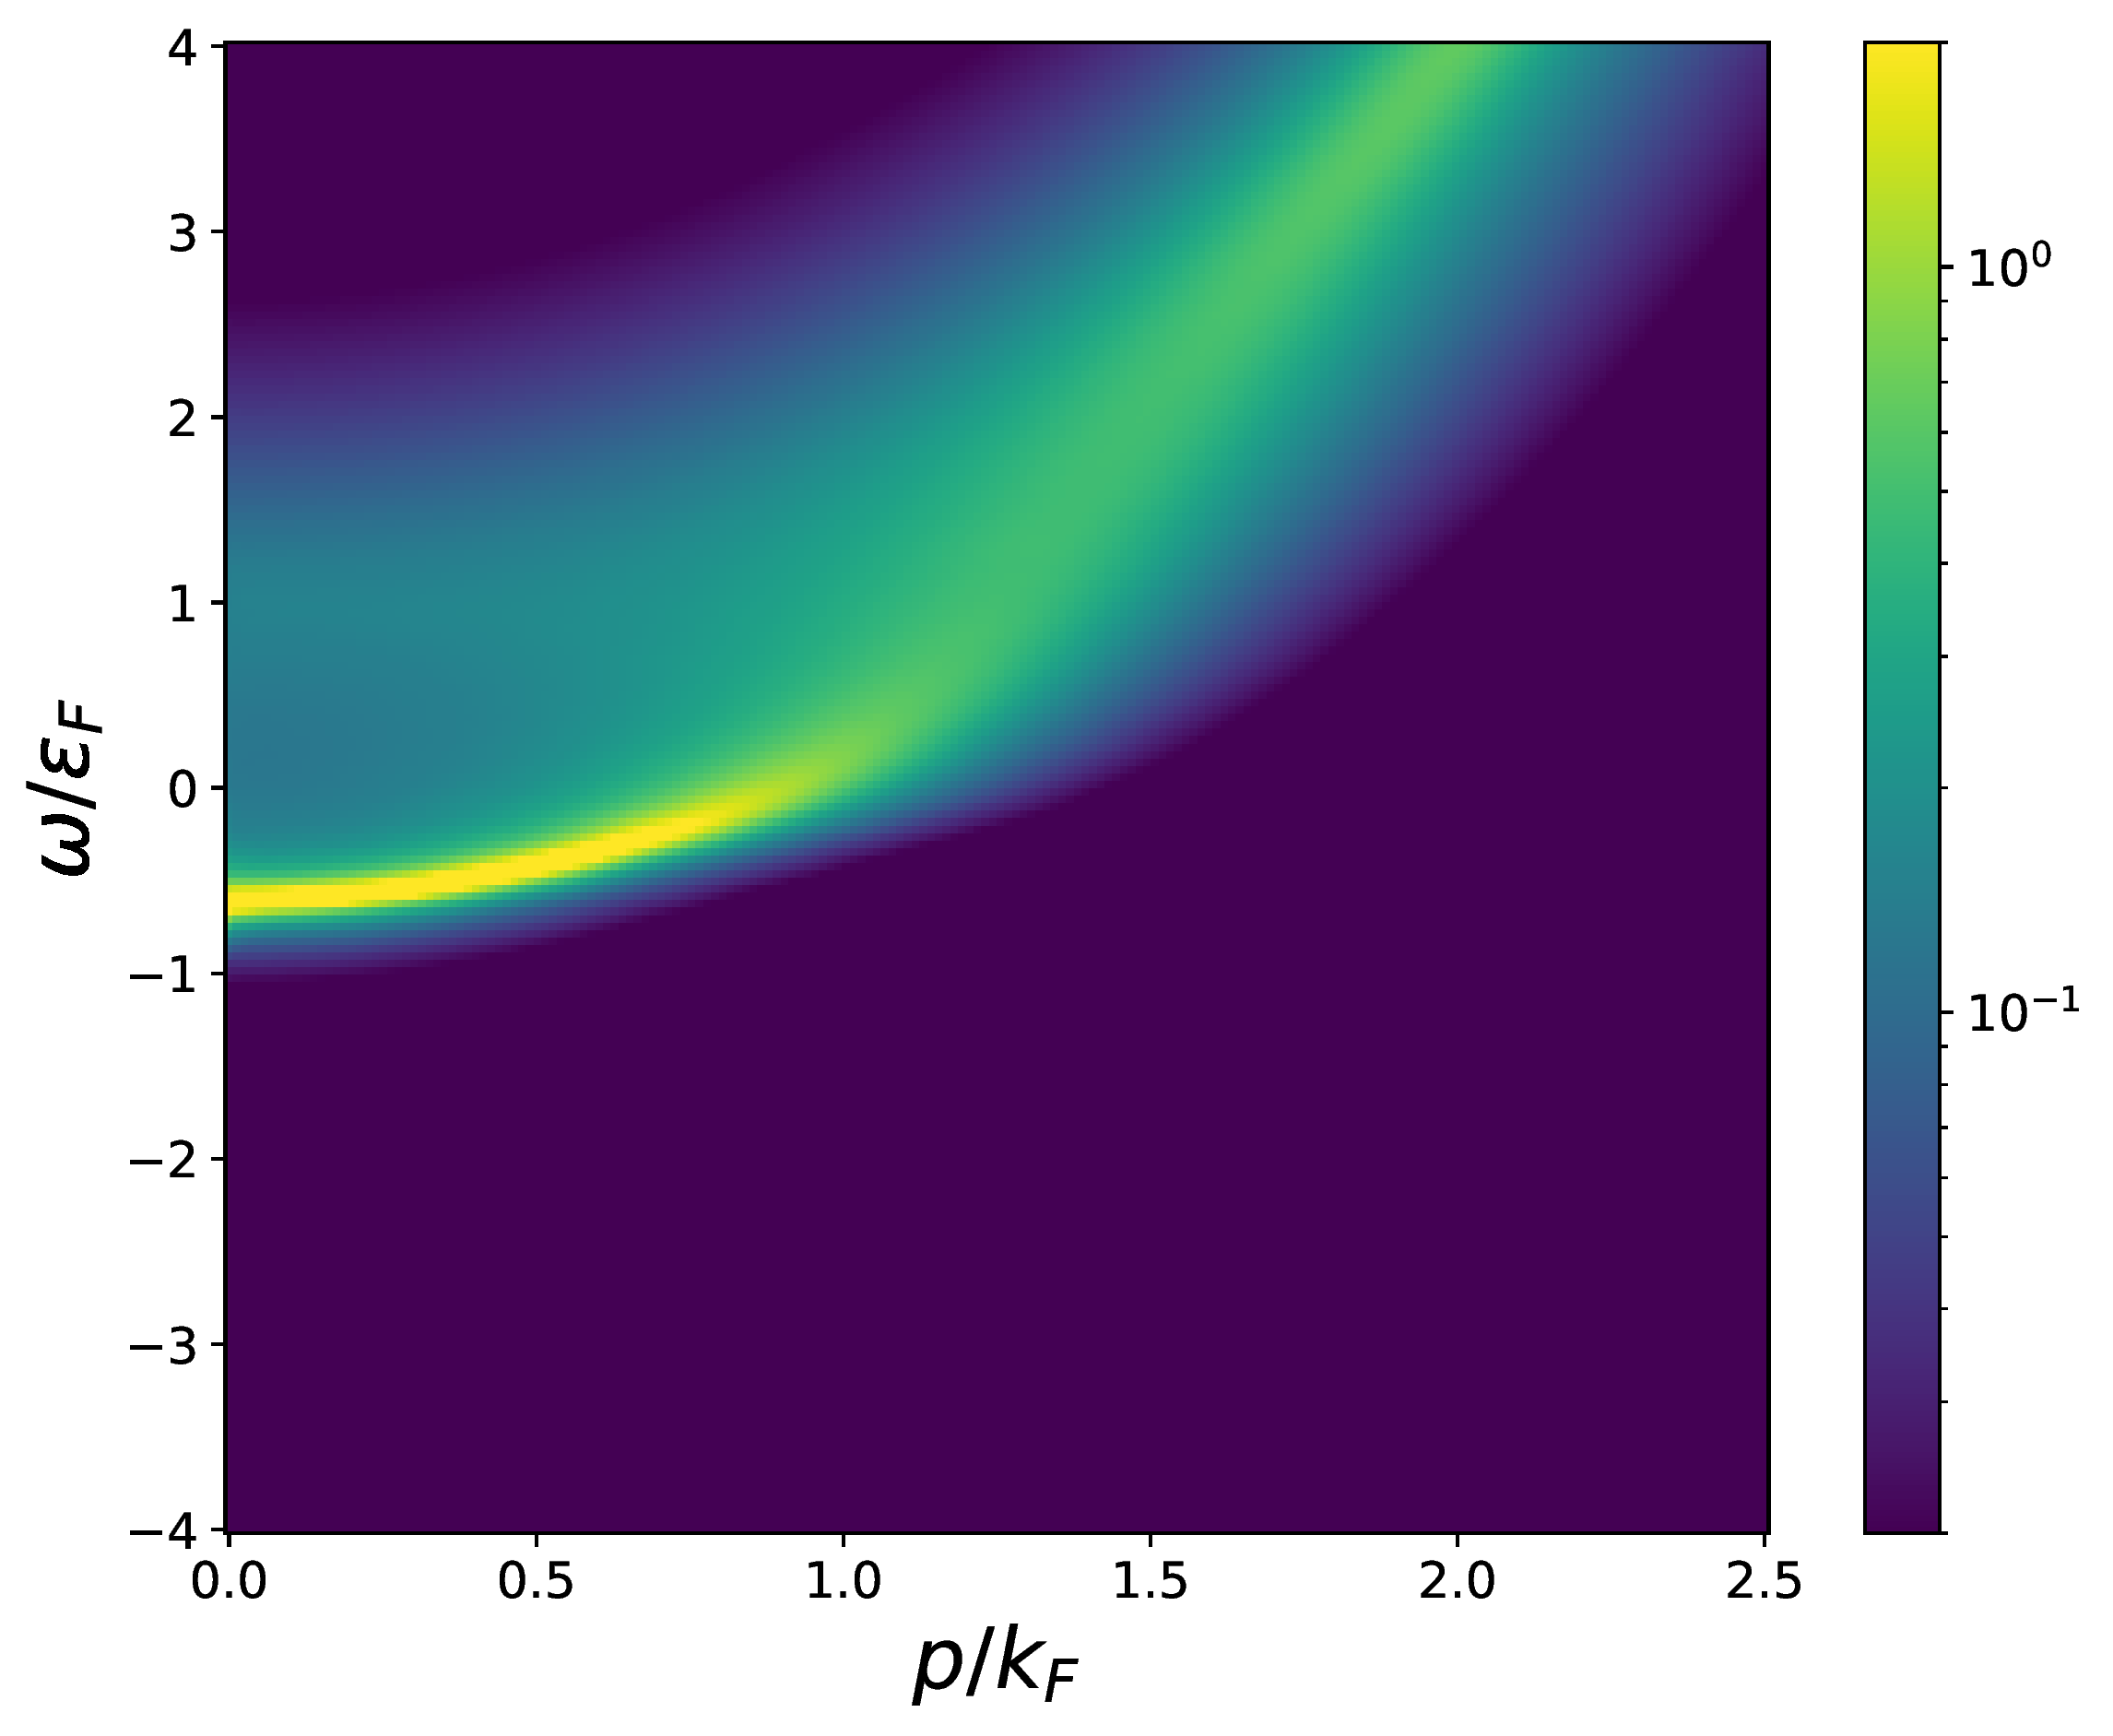
\includegraphics[width=0.24\textwidth]{figs/polaron_unitary0.png}} 
	\subfigure[$(k_Fa)^{-1} = 0.5$]{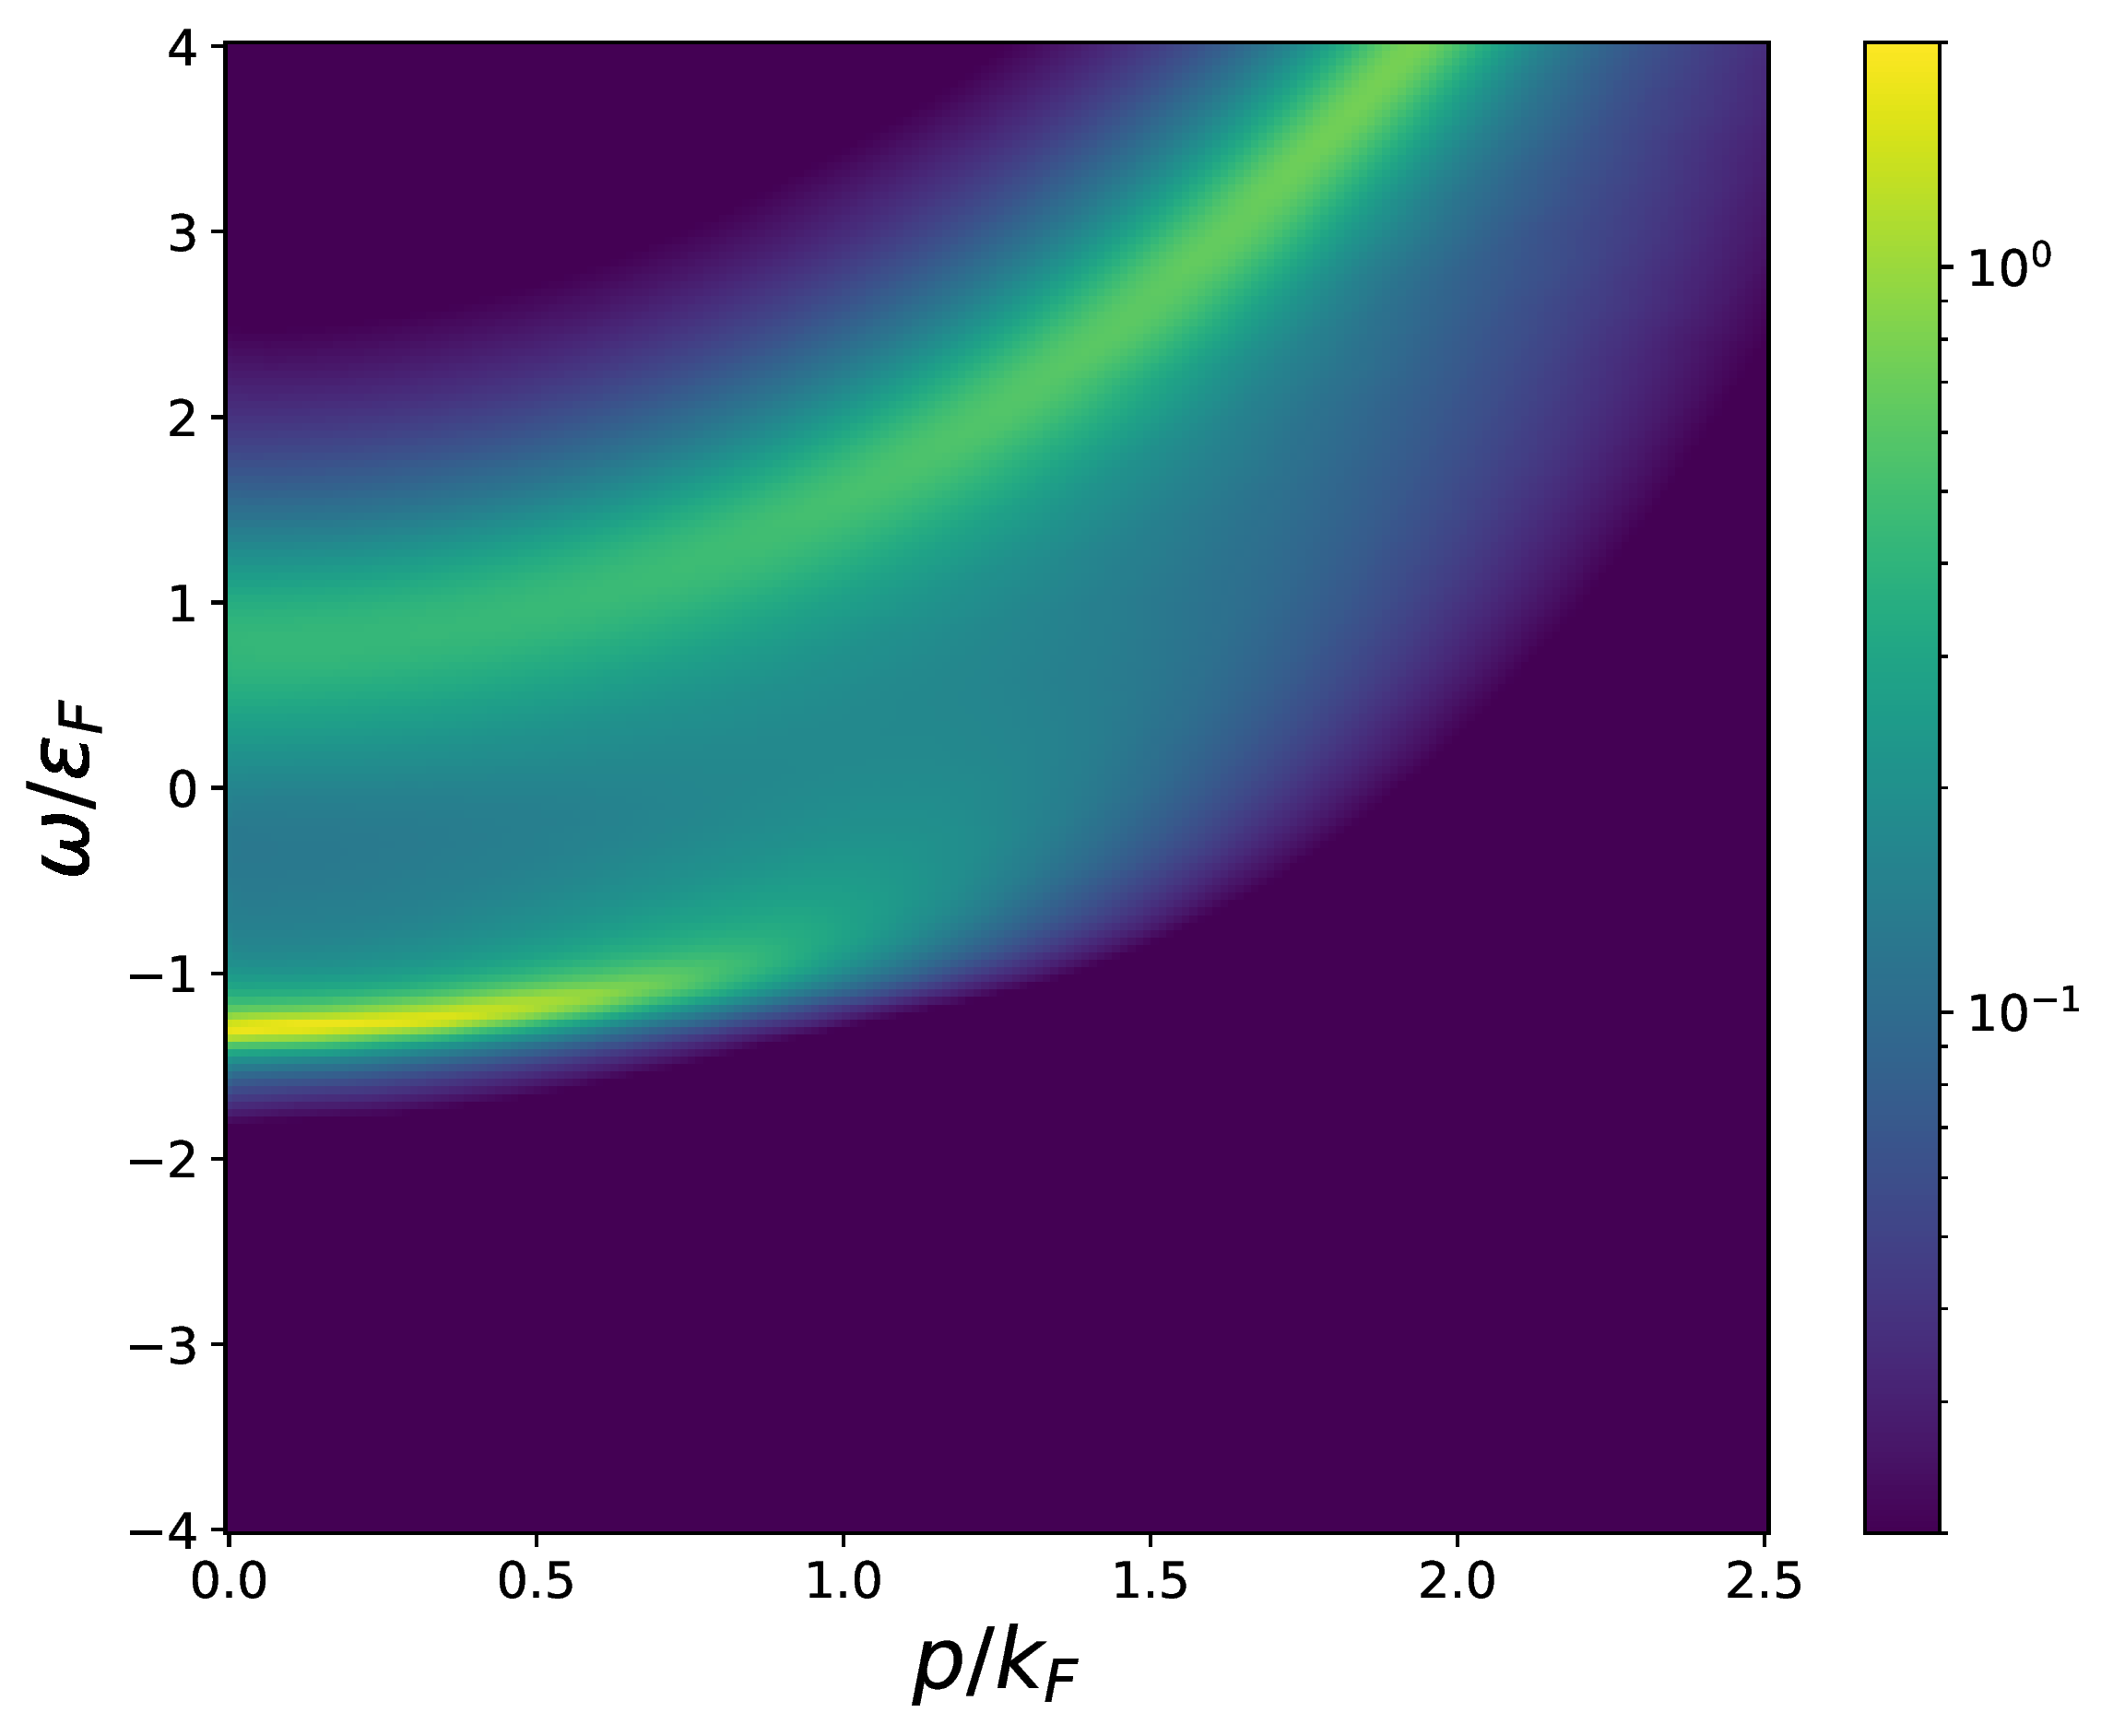
\includegraphics[width=0.24\textwidth]{figs/polaron_05kfa.png}}
	\subfigure[$(k_Fa)^{-1} = 1$]{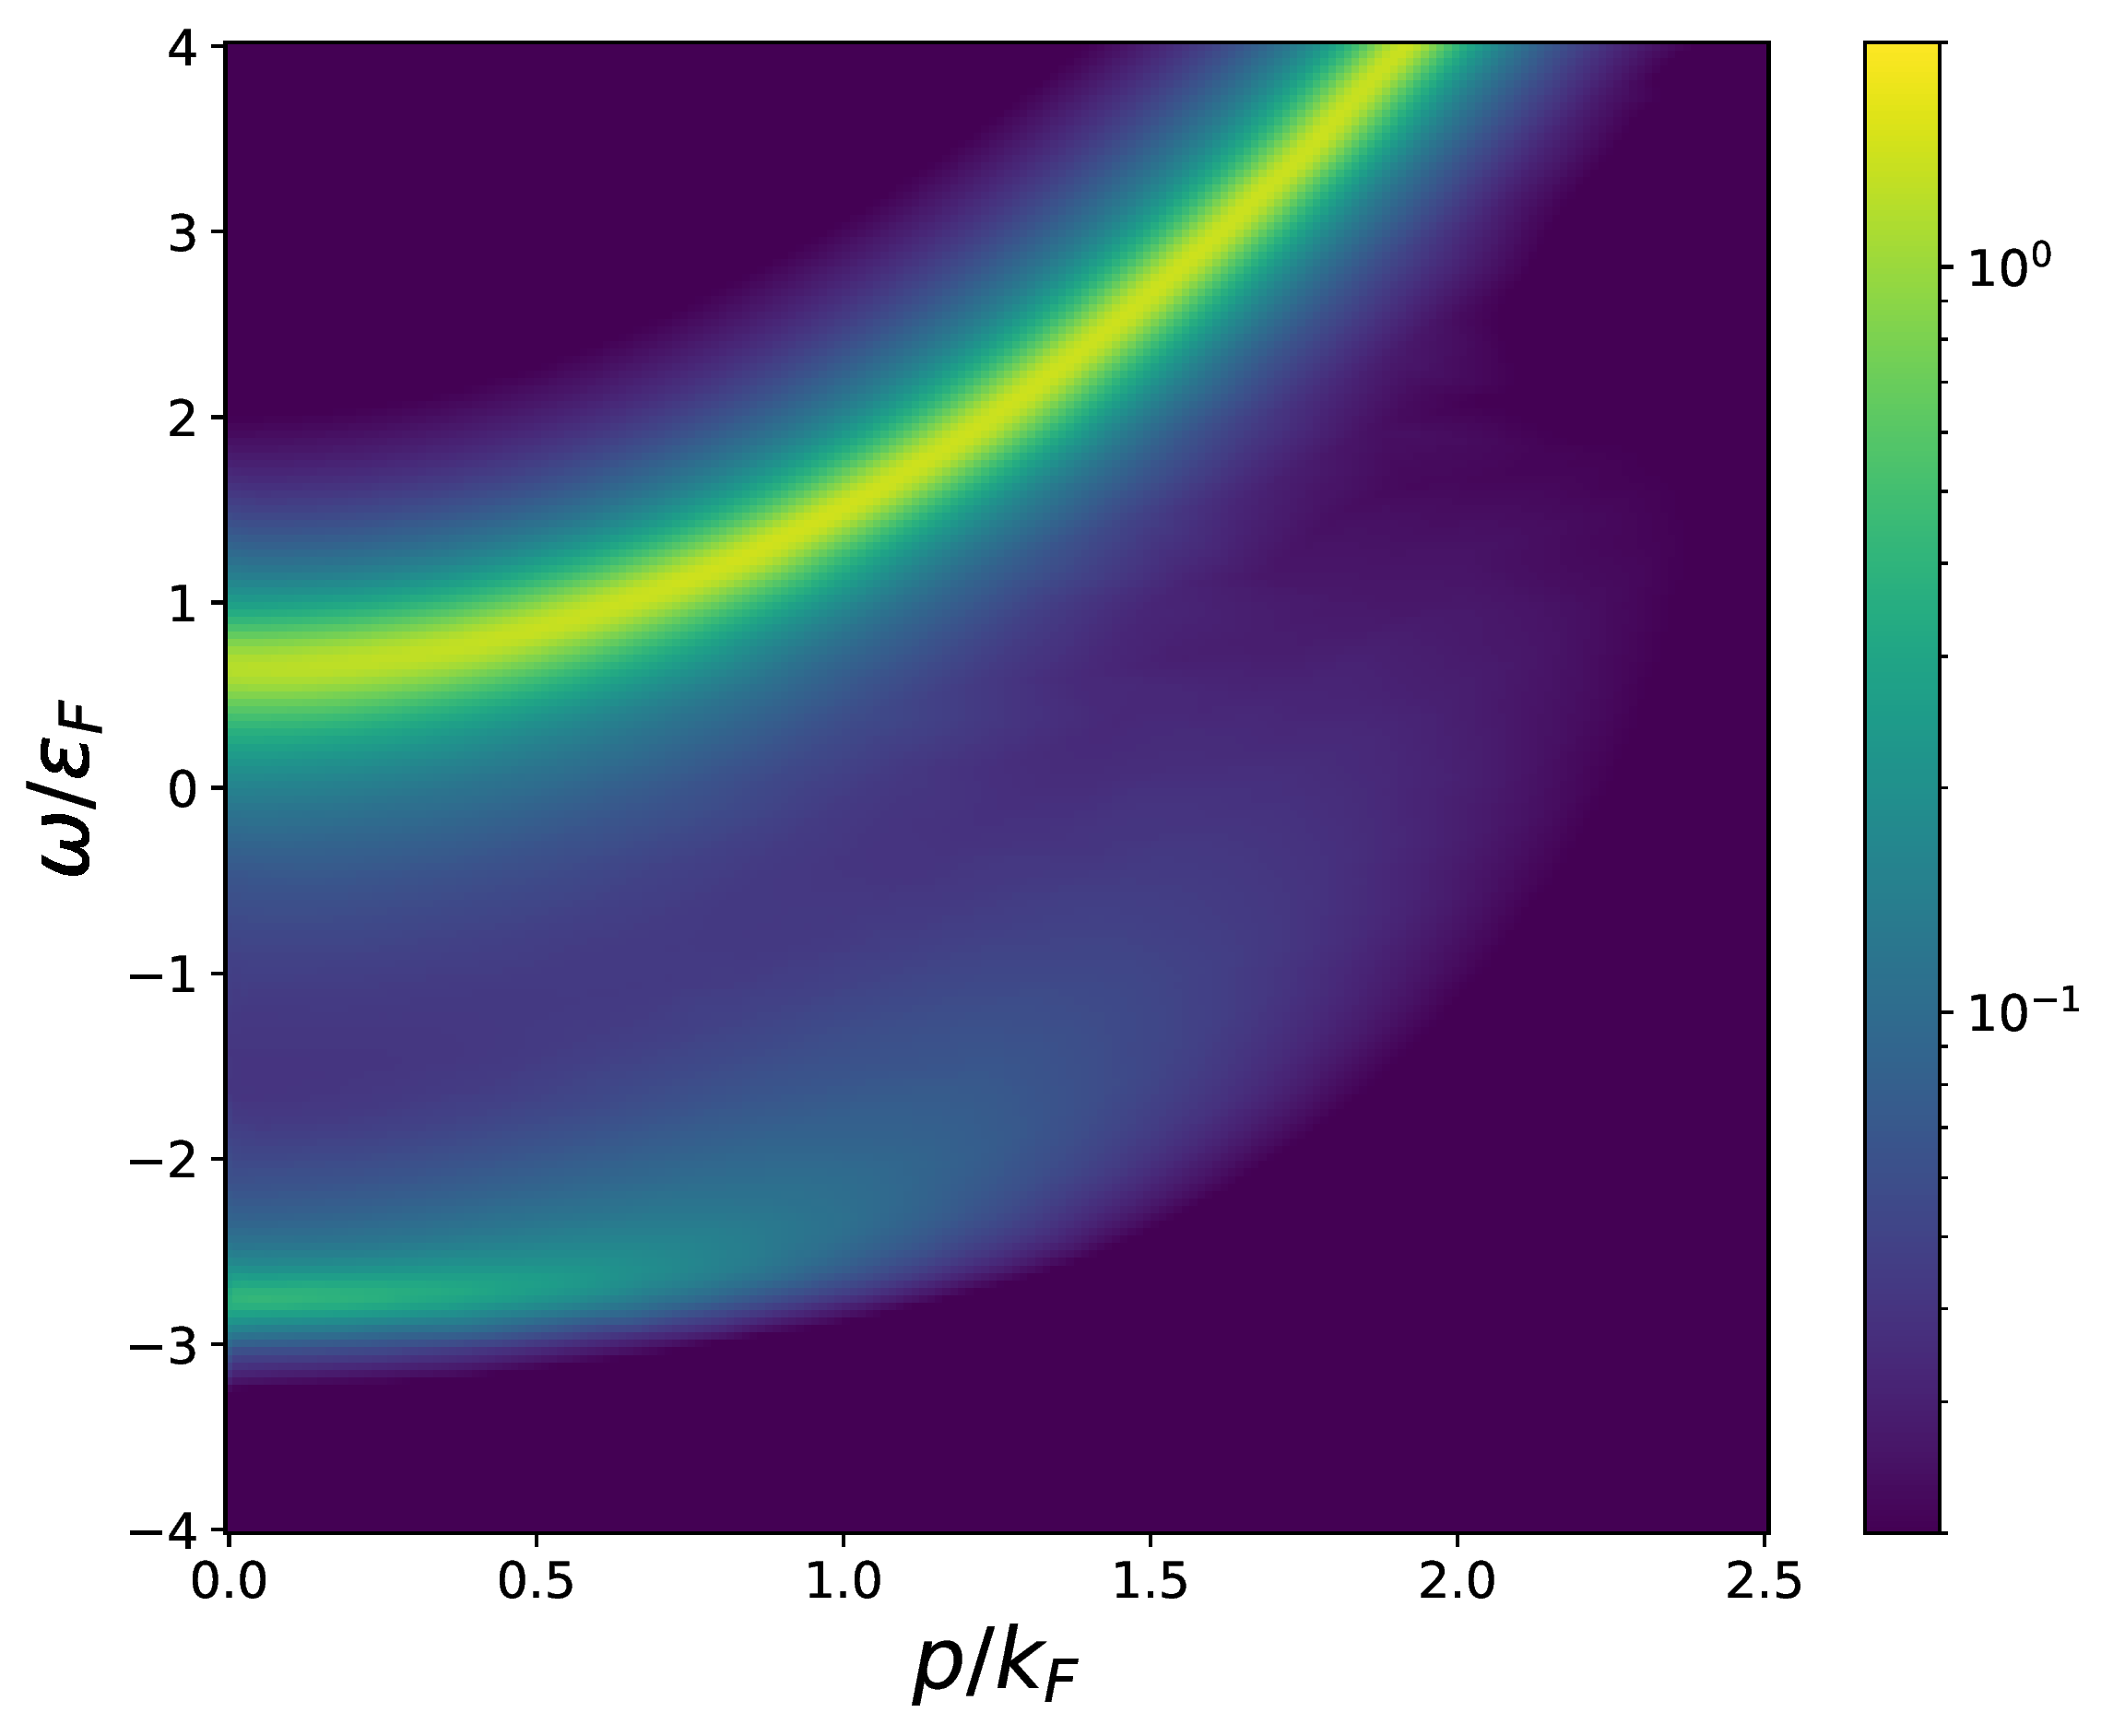
\includegraphics[width=0.24\textwidth]{figs/polaron_1kfa.png}}
	\caption[Spectral functions of Fermi polaron at different interaction strengths]{Results for the Fermi polaron spectral function $\rho_{\downarrow}\,\varepsilon_F$ at $T=0$ at different interaction strengths $(k_Fa)^{-1}$. These results agree well with~\cite{Schmidt2011,Kamikado2017}.}
	\label{fig:specs-comparison}
\end{figure}

From the spectral functions one can obtain important information about the physics of the system. First of all, one can notice the appearance of a second peak for larger interaction strengths $(k_Fa)^{-1}$ while the first one disappears. This is known as the repulsive polaron~\cite{Scazza2022}. Furthermore, one can notice the shift in ground state energy and a changing slope of the attractive polaron peak. Together with the boson ground state energy, the first observation leads to the well-known polaron-to-molecule transition~\cite{Schmidt2011}. The second observation is connected to the divergent effective mass of the attractive polaron~\cite{Vlietinck2013}. For larger interaction strengths the slope gets smaller, which corresponds to a larger effective mass. Eventually, the slope gets zero and can bend back. Besides the effective mass, other quasiparticle properties like the weight $Z$, decay width $\Gamma$ or the contact $C$ can be computed from the spectral function~\cite{Scazza2022}.

Fig.~\ref{fig:effect-finite-temperature} shows the effect of finite temperature in the Fermi polaron problem. One can see that the quasiparticle peak at low momenta gets broadened significantly and slightly shifted. Away from unitarity, one can also observe other phenomena, see~\cite{Hu2022} for more details. Note that the chemical potential $\mu_{\uparrow}(T)$ of the majority particles is temperature-dependent and has to be determined from the number equation for an ideal Fermi gas, see Section~\ref{section:results}. At $T=0.2\,T_F$, the chemical potential is $\mu_{\uparrow}=0.964$. It is compelling to investigate quasiparticle properties as a function of $T$, some of which are considered in~\cite{Hu2022}. One could, for example, compute the quasiparticle weight $Z(T)$ or the contact $C(T)$. It is anticipated that $Z$ should tend to unity for large temperatures, as the spectral function becomes more and more classical. Unfortunately, this analysis could not be finalized before the submission of this Thesis.

In Fig.~\ref{fig:impurity-convergence}, the convergence behavior of the polaron spectral function for two different temperatures is shown. Similar to the spin-balanced BCS-BEC case in Section~\ref{section:results}, the spectral function at higher temperature converges faster and smoother. However, only 5-6 iterations are needed to converge in the polaron case. This is again due to the fact that the majority particles are not dressed and strong correlations do not play a significant role. It is observed that the change from the first to the second iteration is very pronounced, however, further iterations have not so much impact. Other comparisons of non-selfconsistent and selfconsistent results can be found in~\cite{Chien2010,Hu2008,Tajima2021}. In the following, we will make this comparison more explicit by using calculated ejection rf spectra.

Recently, rf spectra and contact of an extremely spin-imbalanced Fermi gas at unitarity were measured at MIT~\cite{Yan2019}. Shortly after, Tajima et al. published first considerations in~\cite{Tajima2019}, and last year Hu et al. published non-selfconsistent real-time results in~\cite{Hu2022}. Here, we want to extend these results to selfconsistent rf spectra.

\begin{figure}[h]
	\centering
	\subfigure[$T=0$]{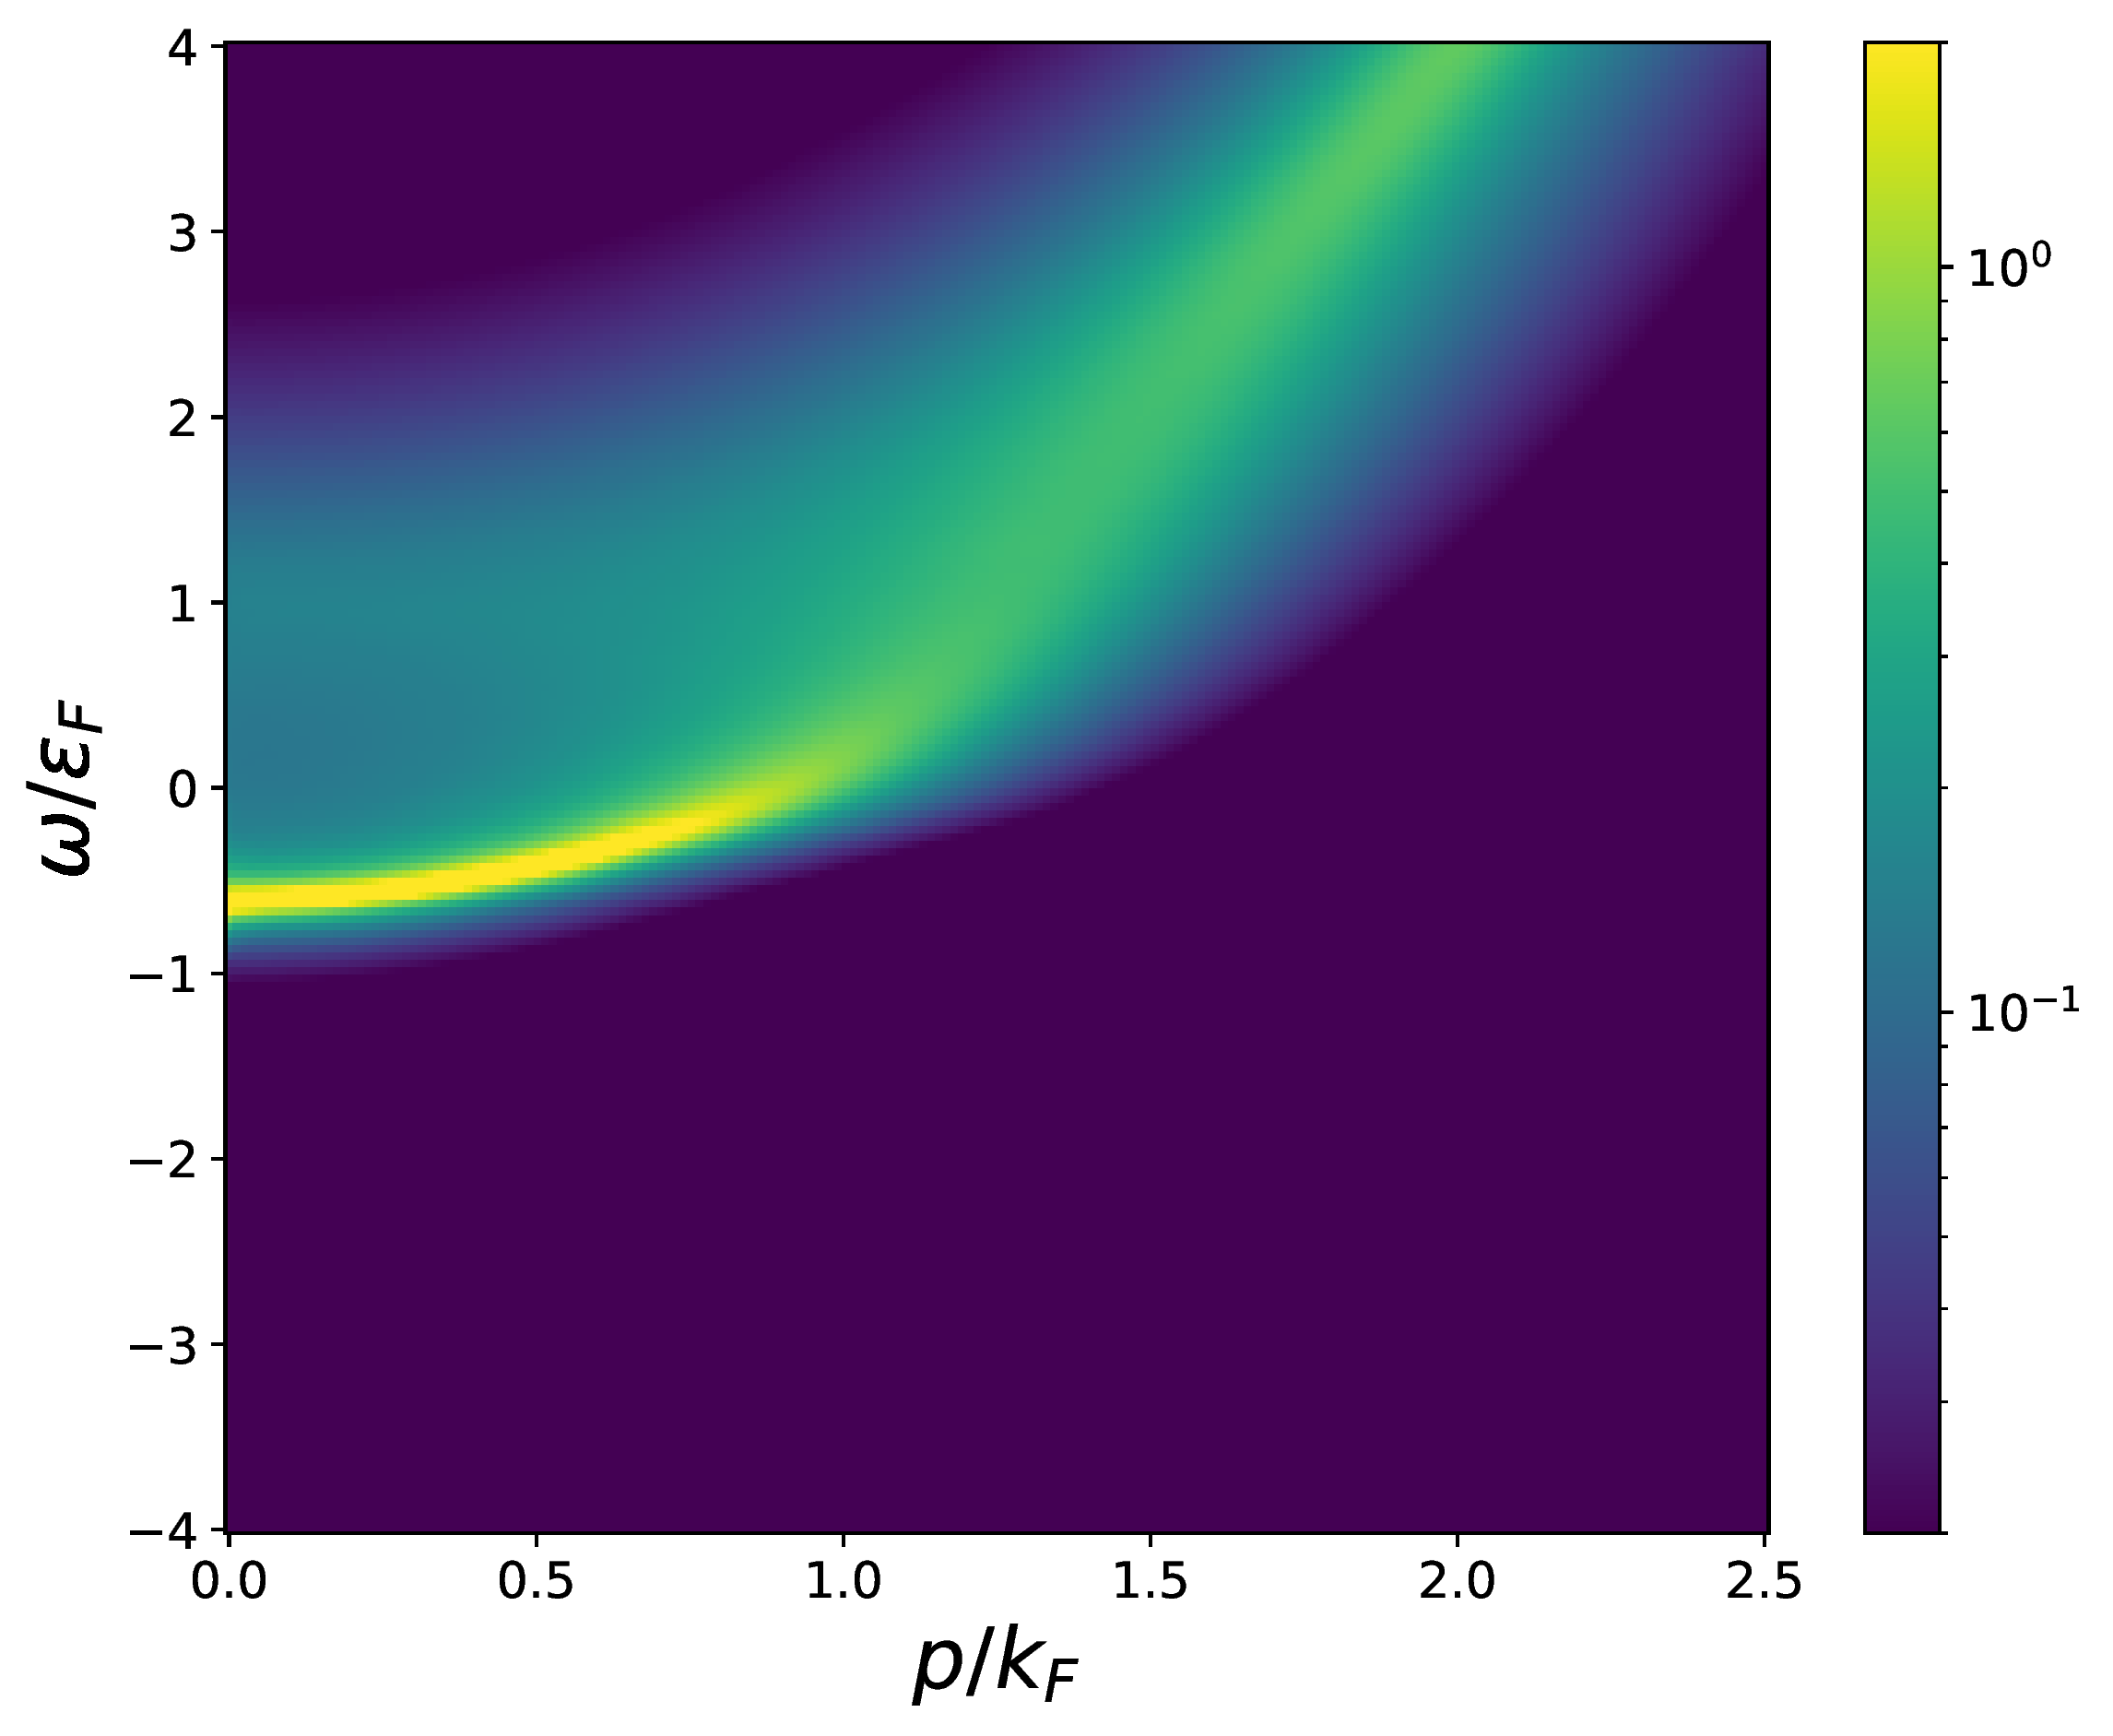
\includegraphics[width=0.468\textwidth]{figs/polaron_unitary0.png}} 
	\subfigure[$T=0.2T_F$]{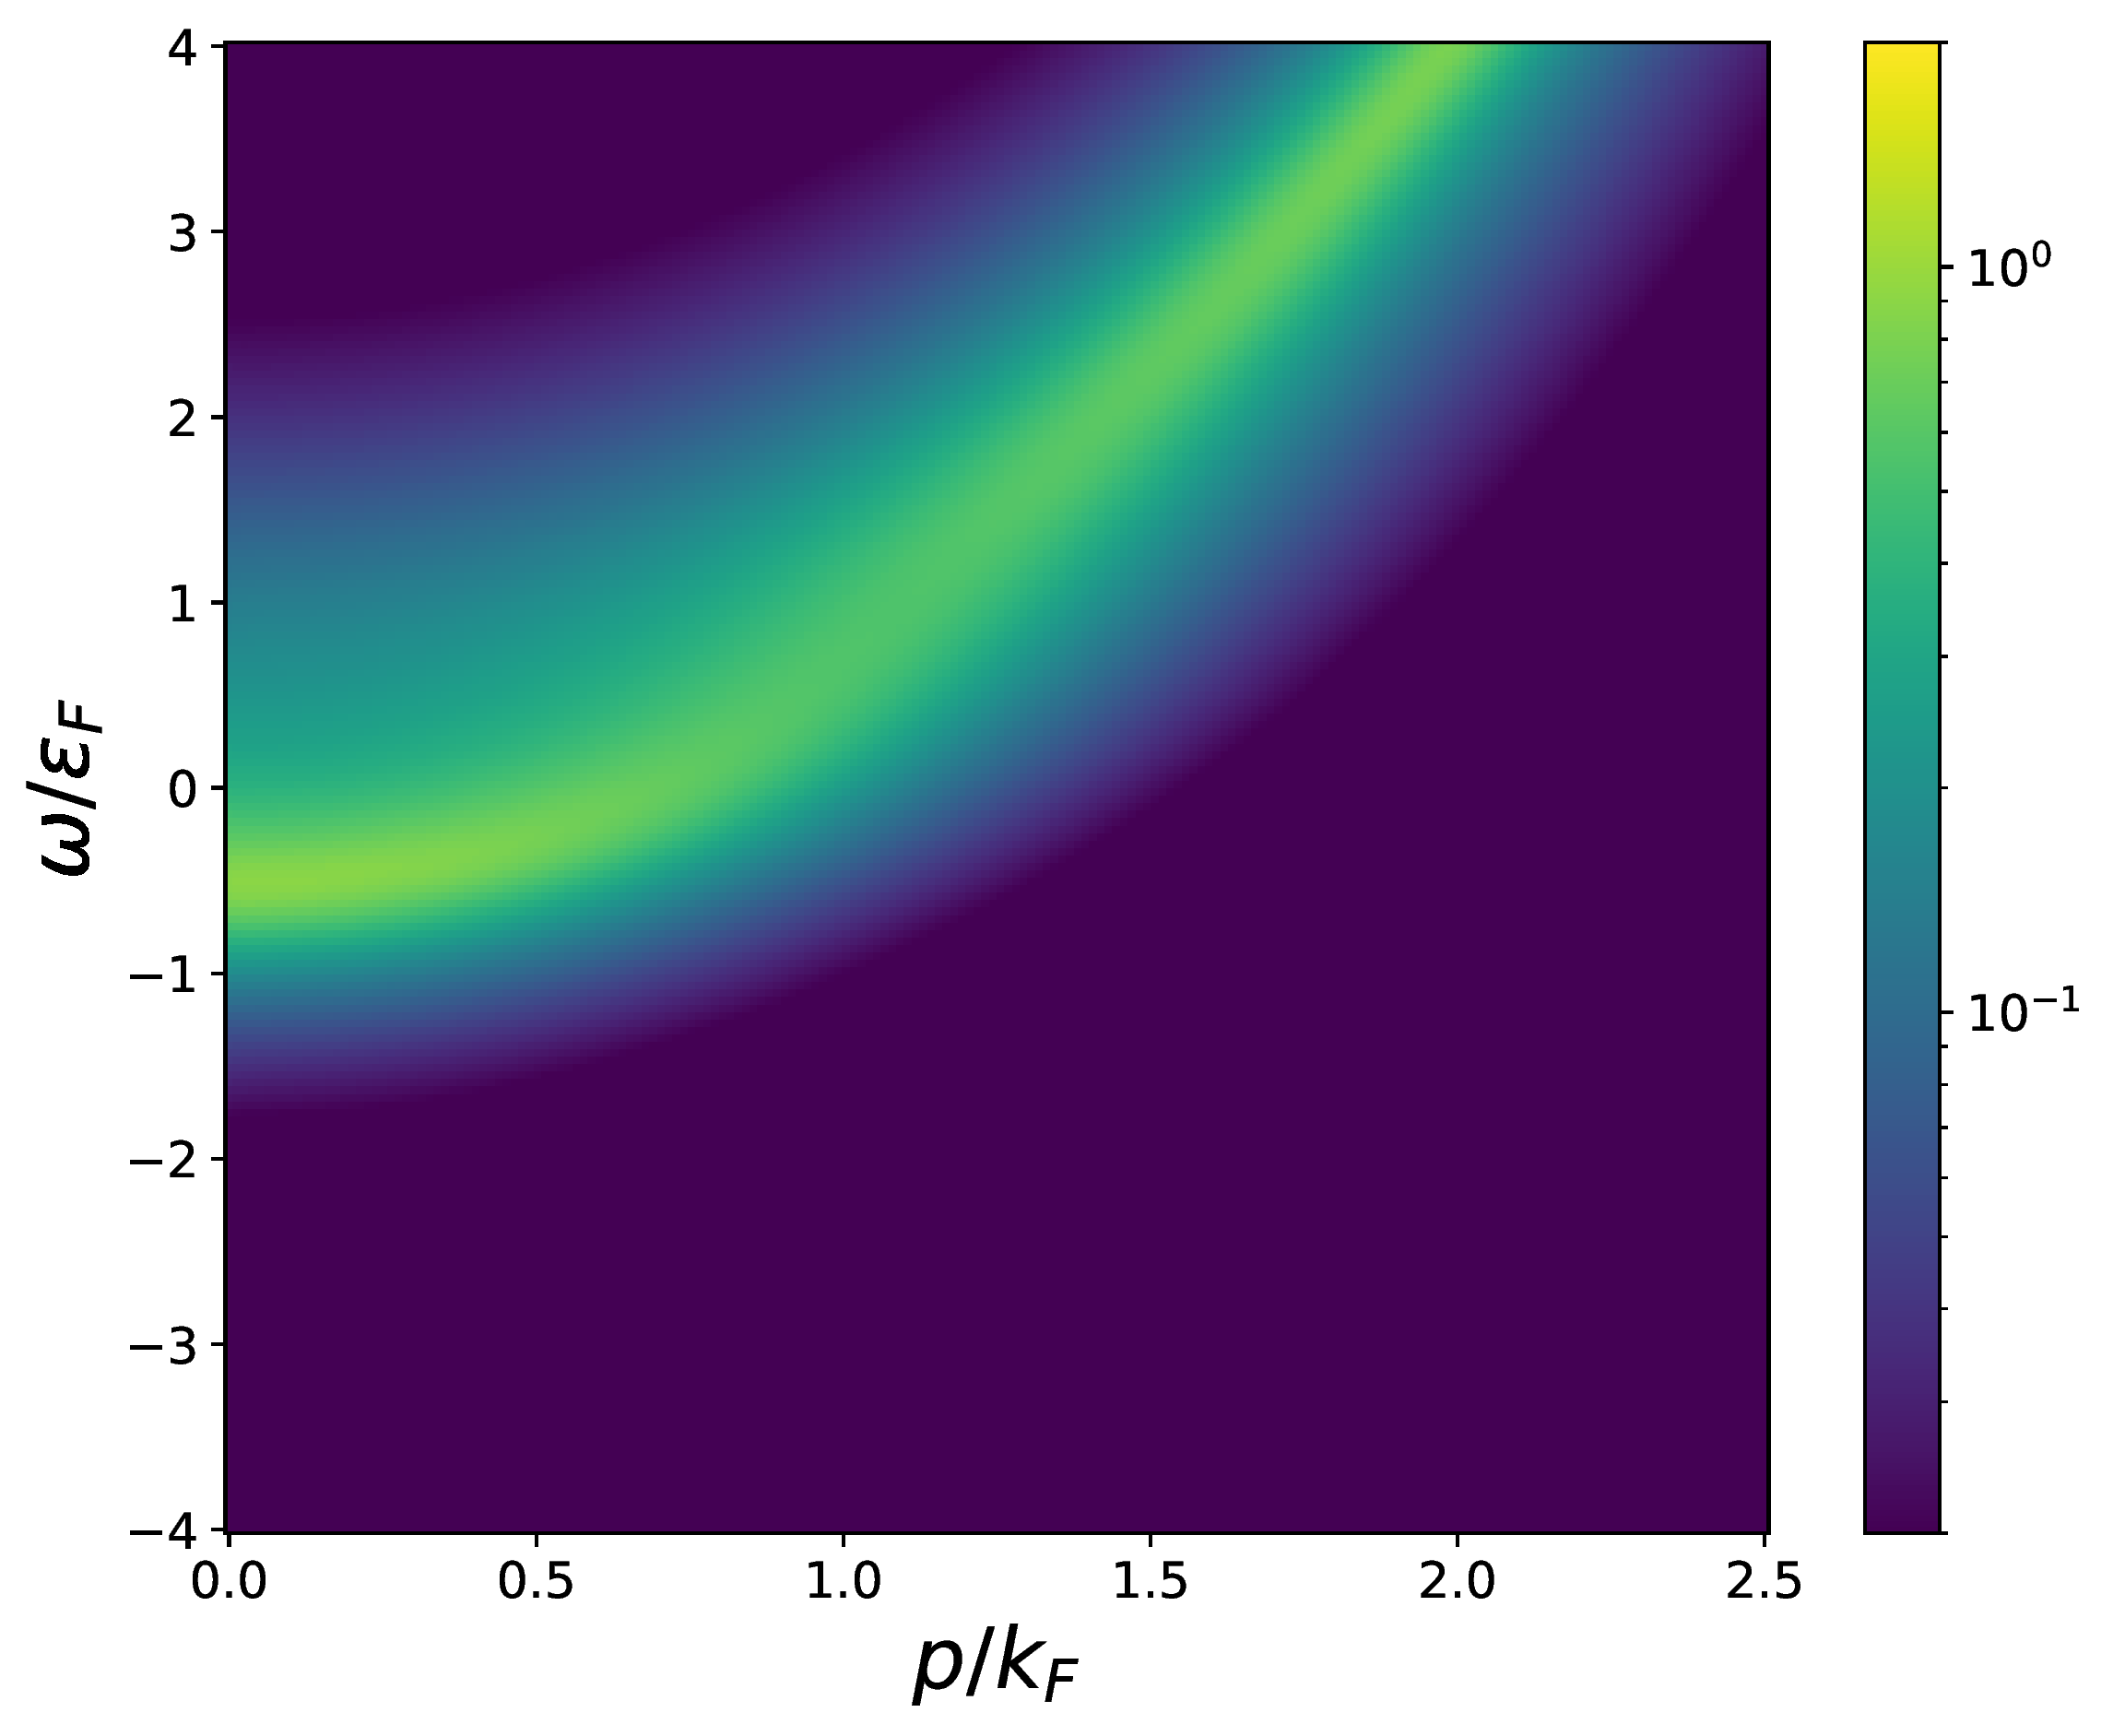
\includegraphics[width=0.468\textwidth]{figs/polaron_unitary02.png}} 
	\caption[Effect of finite temperature]{Effect of finite temperature. Spectral functions of the unitary Fermi polaron at (a) $T=0$ and (b) $T=0.2T_F$.}
	\label{fig:effect-finite-temperature}
\end{figure}

\newpage

\begin{figure}[h]
	\centering
	\subfigure[$T=0.2\,T_F$]{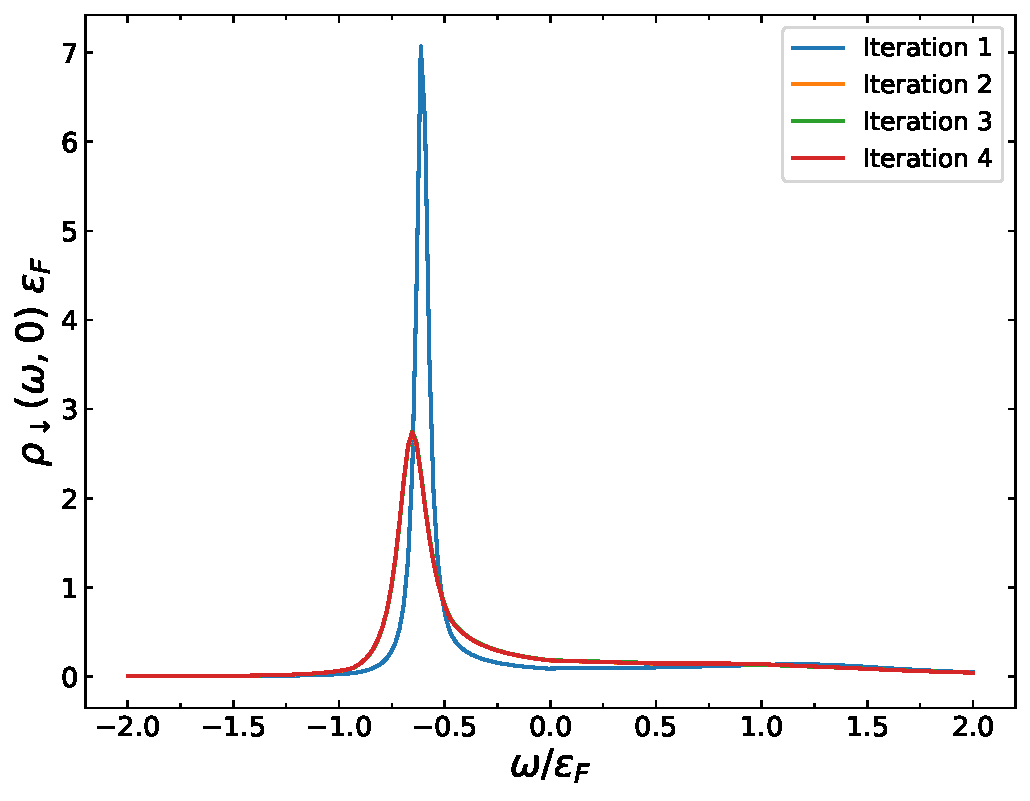
\includegraphics[width=0.468\textwidth]{figs/polaron_unitary02_convergence.pdf}}
	\subfigure[$T=0.8\,T_F$]{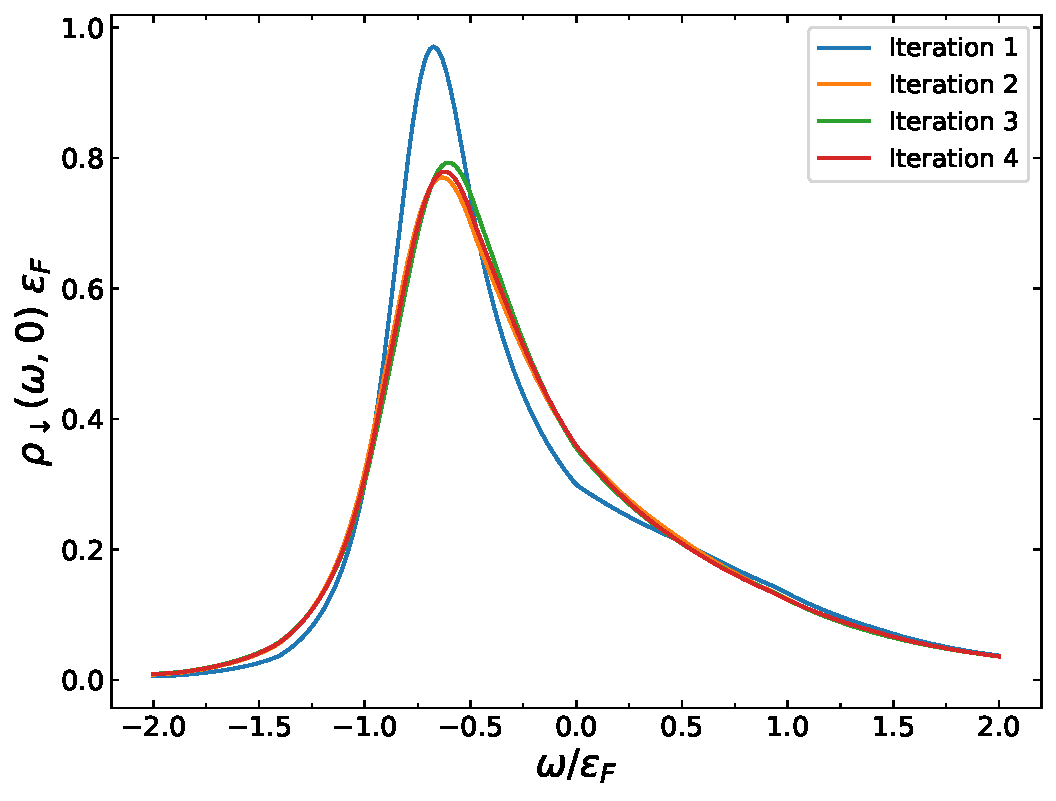
\includegraphics[width=0.476\textwidth]{figs/polaron_unitary08_convergence.pdf}}
	\caption[Convergence of polaron spectral function at different temperatures]{Convergence of the polaron spectral function at different temperatures.}
	\label{fig:impurity-convergence}
\end{figure}

Fig.~\ref{fig:rf-spectra-polaron} shows the non-selfconsistent and selfconsistent results for the polaron rf spectra. These results were obtained in the limit of zero impurity concentration using the same formula~\eqref{eq:rf-spectra} as in Section~\ref{section:results}, see also~\cite{Hu2022,Tajima2019}. For the polaron it reads
%
\begin{align}
	\label{eq:rf-spectra-polaron}
	I(\omega) = \int_{\bm{q}} \rho_{\downarrow}(\varepsilon^{(I)}_{\bm{q}}-\omega-\mu_{\downarrow},\bm{q})\, n_F(\varepsilon^{(I)}_{\bm{q}}-\omega-\mu_{\downarrow}) \,.
\end{align}
%
As mentioned above, we consider the mass-balanced case. The chemical potential of the impurity is $\mu_{\downarrow}=0$. As in the previous Section, the chemical potential of the Fermi sea $\mu_{\uparrow}(T)$ is temperature-dependent and has to be determined from the number equation. Additionally, a Fourier broadening of $0.1\varepsilon_F$ and a right-shift of $0.09\varepsilon_F$ were performed to account for the experimental features. It is found that these results agree well with previous work~\cite{Hu2022,Tajima2019}. However, both approaches cannot describe the experimental data in~\cite{Yan2019} correctly. Since the experimental setup was similar to~\cite{Mukherjee2019}, as discussed in Section~\ref{section:results} for the spin-balanced Fermi gas, the reason for this mismatch might be again the missing trap average for the harmonic trap potential. Other reasons for the mismatch are discussed in~\cite{Hu2022,Tajima2019} and could be due to absent many-body correlations which are not included in the T-matrix approach.

As an outlook for future work, the next step could be to investigate missing three-body correlations~\cite{Bruun2010,Tajima2019}. There exist some approaches to include those effects, however, fully selfconsistent real-time computations are lacking. The spectral method presented in this work provides excellent possibilities to incorporate such three-body diagrams while keeping computational costs quite reasonable. Another possibility would be to include momentum-dependent vertices, as discussed in~\cite{Diehl2006-1, Floerchinger2008, Falco2007, Romans2005, Romans2006}. This was already implemented successfully in the spectral functional approach for scalar field theory~\cite{Horak2020}.


\begin{figure}[htb]
	\begin{minipage}[t]{.492\textwidth}
		\centering
		\subfigure[]{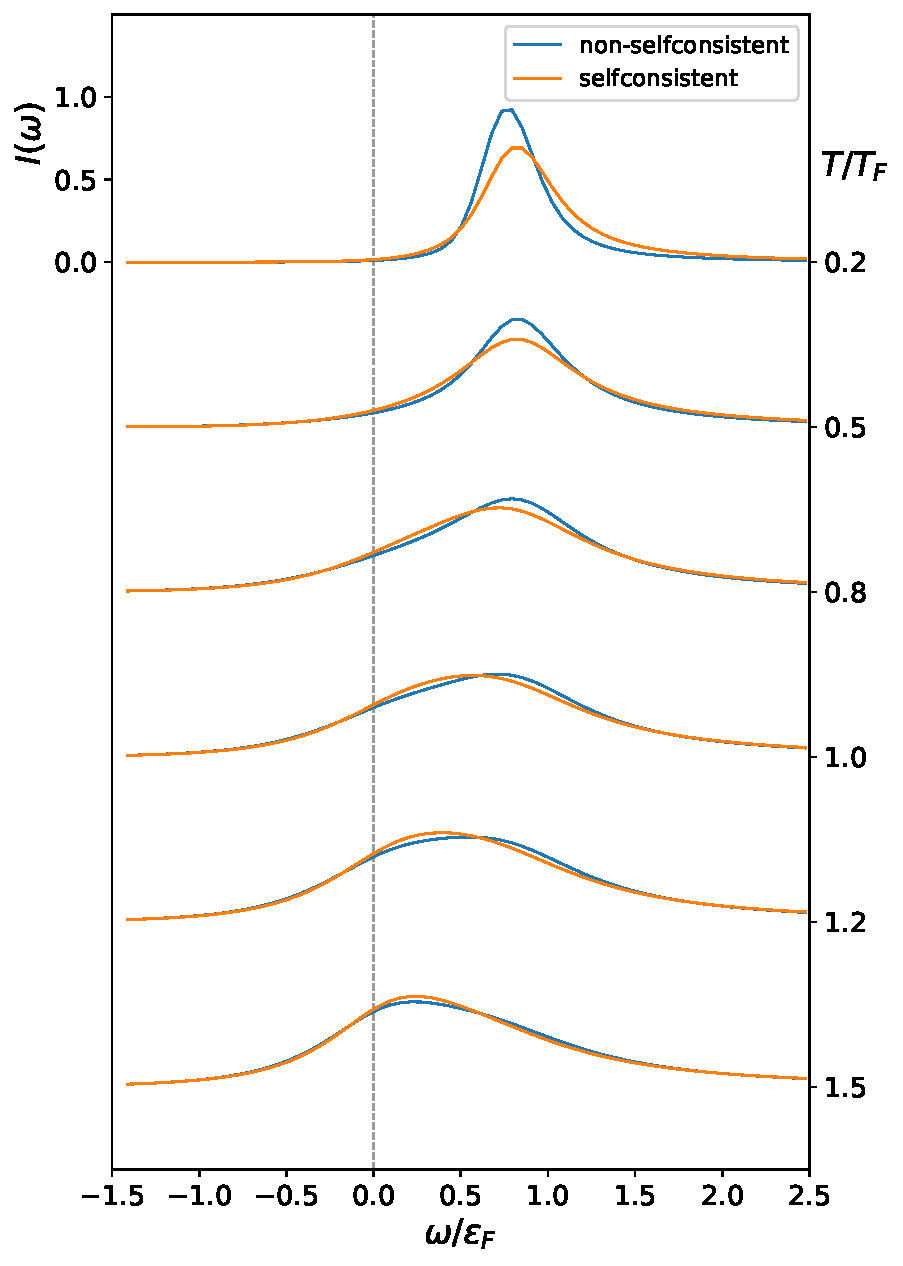
\includegraphics[width=\textwidth]{figs/rf_spectra_polaron.pdf}}
	\end{minipage}
	\hfill
	\begin{minipage}[t]{.49\textwidth}
		\centering
		\subfigure[]{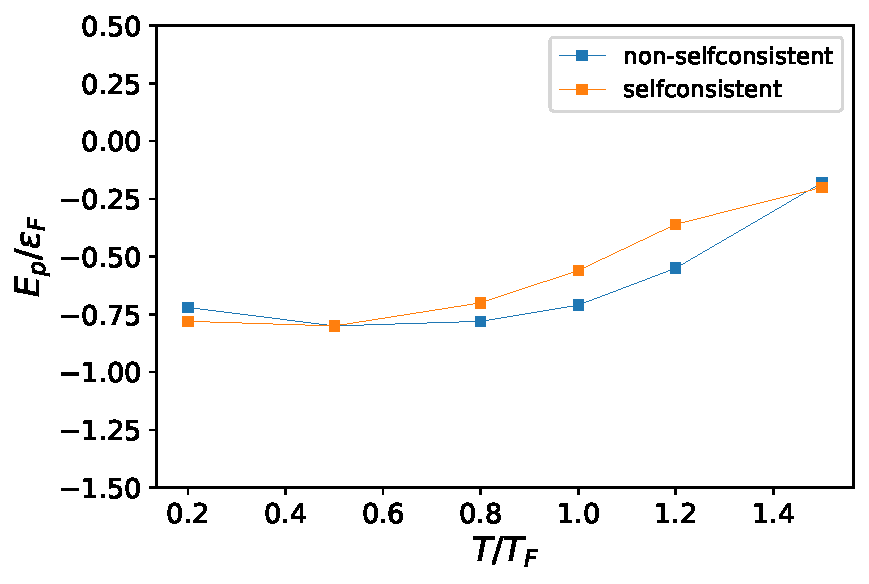
\includegraphics[width=0.95\textwidth]{figs/peakPositions.pdf}}
		\raggedleft
		\subfigure[]{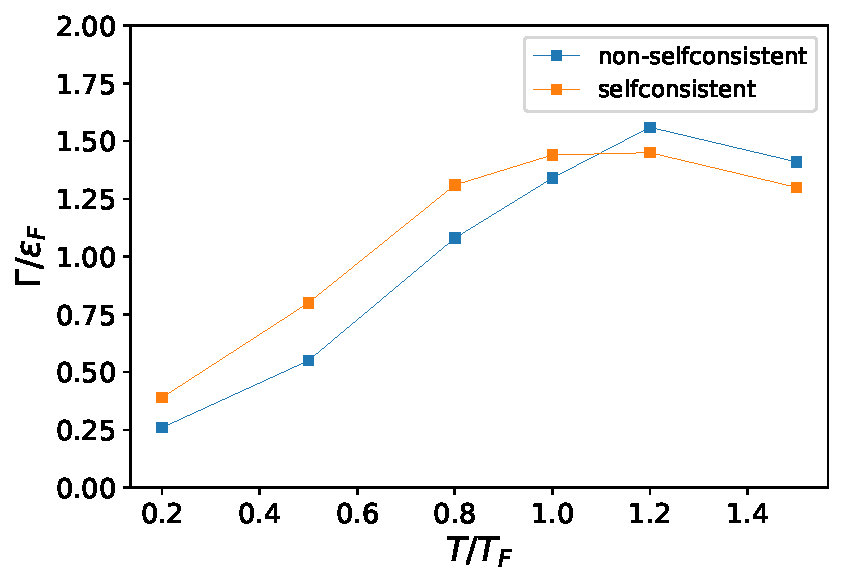
\includegraphics[width=0.92\textwidth]{figs/FWHM.pdf}}
	\end{minipage}
	\caption[Rf spectra of the unitary Fermi polaron]{(a) Calculated ejection rf spectra $I(\omega)$ for the unitary Fermi polaron as a function of the reduced temperature $T/T_F$. Non-selfconsistent results (blue solid lines) are compared to selfconsistent results (orange solid lines). A Fourier broadening of $0.1\varepsilon_F$ to account for the finite experimental resolution, and a right-shift by $0.09\varepsilon_F$ to account for the final state interaction were applied. (b) Peak position ($E_p=-\hbar\omega$) and (c) full width at half maximum $\Gamma$ extracted from the rf spectra.}
	\label{fig:rf-spectra-polaron}
\end{figure}
	\chapter{Conclusion and Outlook}
\label{chapter:conclusion}

In this Thesis, we calculated spectral functions of strongly interacting Fermi gases directly in real frequencies without the need of numerical reconstruction methods by iteratively solving the corresponding Dyson-Schwinger equations. 

In the first part, we focused on the spectral properties of the spin-balanced BCS-BEC crossover. After introducing the basic theoretical foundations in Chapter~\ref{chapter:functional-methods} and~\ref{chapter:ultracold-gases}, we presented the main achievements of this work in Chapter~\ref{chapter:bcs-bec-crossover}. A fully selfconsistent numerical framework in real frequencies was developed. Additionally, analytic results for the non-selfconsistent boson self-energy with general mass and spin-imbalance at zero and finite temperature were derived. Novel results for the bosonic dimer and the fermionic single-particle spectral functions in the normal phase of the BCS-BEC crossover phase diagram were obtained. To benchmark our calculations, we applied our method to the unitary Fermi gas and compared with existing theoretical predictions and experimental data. Excellent agreement with previous work in the normal phase is found. The symmetry-broken phase turns out to be more challenging and requires additional work in the future.

In the second part, we applied our selfconsistent real-time framework to the Fermi polaron problem in Chapter~\ref{chapter:fermi-polaron}. In this case, some simplifications could be made which reduced the number of integrals and improved the numerical performance. Previous fRG and T-matrix results were confirmed and extended. Despite employing a selfconsistent approach, the experimental data could not be described accurately. The reason for this might involve the lack of many-body correlations, which can be investigated with the spectral approach.

The results obtained in this work promise a wide range of possible applications, including transport properties and the ab-initio calculation of spectral functions in the superfluid phase of the BCS-BEC crossover. Moreover, the numerical framework can be extended to full momentum-dependent vertices, or general mass and spin-imbalance. The spectral approach can be used to study various quasiparticle properties of strongly interacting Fermi gases at finite temperature. Also more involved processes like three-body scattering diagrams can be considered in the future.

\cleardoublepage


%Appendices
\appendix{
	\chapter{Appendix}

\section{Propagators}
\label{app:propagators}

In this Appendix, we derive the classical propagators in superfield notation~\cite{Pawlowski2021}.

The full action of the single-channel model~\eqref{eq:single-channel-action} in position space is~\cite{Boettcher2012}
\begin{align}
    S[\psi, \phi] &= \int_{X,Y} \psi^*_i(Y)
    \left[\left(-\partial_{\tau} - \nabla_X^2 - \mu\right) \delta(X-Y)\right] \psi_i(X) \notag \\
    &+ \int_{X,Y} \phi^*(Y)
    \left[\nu\, \delta(X-Y)\right] \phi(X) \notag \\
    &+ \int_{X,Y,Z} \left[-h \, \delta(Z-X) \delta(Y-X)\right]
	\phi^*(Z) \psi_1(Y) \psi_2(X) \notag \\
	&+ \int_{X,Y,Z} \left[h \, \delta(Z-X) \delta(Y-X)\right]
	\phi(Z) \psi_1^*(Y) \psi_2^*(X) \,.
\end{align}

Defining the Fourier transforms
\begin{align}
    \psi(X) = \int_Q \psi(Q) e^{-iQX} \,, \quad
    \psi^*(X) = \int_Q \psi^*(Q) e^{iQX} \,.
\end{align}

The full action in momentum space is
\begin{align}
    S[\psi, \phi] &= \int_{Q,Q'} \psi^*_i(Q)
    \left[(-i\omega_n + q^2 - \mu) \delta(Q-Q')\right] \psi_i(Q') \notag \\
    &+ \int_{Q,Q'} \phi^*(Q)
    \left[\nu\, \delta(Q-Q')\right] \phi(Q') \notag \\
    &+ \int_{Q,Q',Q''} \left[-h \, \delta\left(Q - (Q'+Q'')\right)\right]
	\phi^*(Q) \psi_1(Q') \psi_2(Q'') \notag \\
	&+ \int_{Q,Q',Q''} \left[h \, \delta\left(Q - (Q'+Q'')\right)\right]
	\phi(Q) \psi_1^*(Q') \psi_2^*(Q'') \,.
\end{align}


In superfield notation~\cite{Pawlowski2021}, we can write the action as
\begin{align}
	\label{eq:superfield-action}
    S[\Phi] &= S^{\psi_i\psi^*_i} \psi^*_i\psi_i + S^{\phi\phi^*} \phi^*\phi
    + S^{\psi_2\psi_1\phi^*} \phi^*\psi_1\psi_2 + S^{\psi^*_2\psi^*_1\phi}
    \phi\psi^*_1\psi^*_2 \,,
\end{align}
where the classical propagators in momentum space are given by
\begin{align}
    S^{\psi_i\psi^*_i} &= \frac{\delta}{\delta\psi_i}\frac{\delta}{\delta\psi^*_i} S[\Phi] 
    = (-i\omega_n + q^2 - \mu) \delta(Q-Q') \,, \notag \\
    S^{\phi\phi^*} &= \frac{\delta}{\delta\phi}\frac{\delta}{\delta\phi^*} S[\Phi]
    = \nu\, \delta(Q-Q') \,, \notag \\
    S^{\psi_2\psi_1\phi^*} &= \frac{\delta}{\delta\psi_2}\frac{\delta}{\delta\psi_1}
    \frac{\delta}{\delta\phi^*} S[\Phi] 
    = -h \, \delta\left(Q - (Q'+Q'')\right) \,, \notag \\
    S^{\psi^*_2\psi^*_1\phi} &= \frac{\delta}{\delta\psi^*_2}\frac{\delta}{\delta\psi^*_1}
    \frac{\delta}{\delta\phi} S[\Phi]
    = h \, \delta\left(Q - (Q'+Q'')\right) \,.
\end{align}
We can also check that the anomalous components are given by
\begin{align}
	S^{\phi\phi} &= \frac{\delta}{\delta\phi}\frac{\delta}{\delta\phi} S[\Phi] = 0 \,, \notag \\
	S^{\phi^*\phi^*} &= \frac{\delta}{\delta\phi^*}\frac{\delta}{\delta\phi^*} S[\Phi] = 0 \,, \notag \\
	S^{\psi_1\psi_2} &= \frac{\delta}{\delta\psi_1}\frac{\delta}{\delta\psi_2} S[\Phi] 
	= h\, \phi^*(Q)\, \delta\left(Q - (Q'+Q'')\right) \,, \notag \\
	S^{\psi^*_2\psi^*_1} &= \frac{\delta}{\delta\psi^*_2}\frac{\delta}{\delta\psi^*_1} S[\Phi]
	= h\, \phi(Q)\, \delta\left(Q - (Q'+Q'')\right) \,.
\end{align}

Note that for fermions and bosons
\begin{align}
    \int_X \psi^*_i(X) \left(\partial_{\tau} - \nabla^2 - \mu\right) \psi_i(X)
    &= \int_X \psi_i(X) \left(\partial_{\tau} + \nabla^2 + \mu\right) \psi^*_i(X) \,, \notag \\
    \int_X \phi^*(X) \left(\partial_{\tau} - \nabla^2 - \mu\right) \phi(X)
    &= \int_X \phi(X) \left(-\partial_{\tau} - \nabla^2 - \mu\right) \phi^*(X) \,,
\end{align}
and therefore the two-point functions satisfy the symmetries
\begin{align}
    S^{\psi^*_i\psi_i}(P) = -S^{\psi_i\psi^*_i}(-P) \,, \qquad
    S^{\phi^*\phi}(P) = S^{\phi\phi^*}(-P) \,,
\end{align}
whereas the three-point function does not contain any derivatives
and is anti-symmetric in the fermionic fields, e.g.,
\begin{align}
    S^{\psi_1\psi_2\phi^*} = -S^{\psi_2\psi_1\phi^*}  \,.
\end{align}

The anomalous propagators satisfy the following symmetries, see also~\cite{Frank2018},
\begin{align}
	S^{\psi_1\psi_2}(P) = S^{\psi^*_2\psi^*_1}(-P)^* \,, \qquad 
	S^{\phi\phi}(P) = S^{\phi^*\phi^*}(-P)^* \,.
\end{align}

\clearpage

\section{Derivation of DSEs}
\label{app:derivation-dse}

In this Appendix, we derive the Dyson-Schwinger equations for the propagators.

The starting point is the general DSE in Eq.~\eqref{eq:DSE-general}, see also~\cite{Pawlowski2021},
\begin{align}
	\frac{\delta\Gamma\left[\Phi\right]}{\delta\Phi_a} =
	\frac{\delta S}{\delta\phi_a}\left[ \phi_b = \Phi_b
	+ G_{bc} \cdot \frac{\delta}{\delta \Phi_c} \right] \,.
\end{align}
Applying this formula to the action~\eqref{eq:superfield-action} in superfield notation yields, e.g., for the fermion propagator
\begin{align}
	\frac{\delta S}{\delta\psi^*_1} = S^{\psi_1\psi^*_1} \psi_1 +
	S^{\psi^*_2\psi^*_1\phi} \phi\psi^*_2 \,.
\end{align}
In terms of the effective fields:
\begin{align}
	\frac{\delta\Gamma}{\delta\Psi_1^*} &=
	S^{\psi_1\psi^*_1} \left[\Psi_1 + G_{\psi_1 k}
	\cdot \frac{\delta}{\delta \Phi_k} \right]
	+ S^{\psi^*_2\psi^*_1\phi} \left[\Phi + G_{\phi l}
	\cdot \frac{\delta}{\delta \Phi_l} \right]
	\left[\Psi^*_2 + G_{\psi^*_2 m}
	\cdot \frac{\delta}{\delta \Phi_m} \right] \notag \\
	&= S^{\psi_1\psi^*_1} \Psi_1 + S^{\psi^*_2\psi^*_1\phi} \Phi \Psi^*_2
	+ S^{\psi^*_2\psi^*_1\phi} G_{\phi \psi^*_2} \,.
\end{align}
Applying another $\delta/\delta\Psi_1$ derivative yields
\begin{align}
	\frac{\delta^2\Gamma}{\delta\Psi_1\delta\Psi_1^*} =
	S^{\psi_1\psi^*_1} + S^{\psi^*_2\psi^*_1\phi}
	\frac{\delta}{\delta\Psi_1} G_{\phi \psi^*_2} \,.
\end{align}
Now, we can use the fact that~\cite{Wink2020}
\begin{align}
	G_{ac} \cdot \Gamma^{cb}
	= (-1)^{ab} \delta^a_b \,,
\end{align}
and therefore~\cite{Pawlowski2021} 
\begin{align}
	\frac{\delta}{\delta\Phi_a} G_{b c}
	= - (-1)^{ab} (-1)^{ee} G_{bd} \cdot \Gamma^{dae} \cdot G_{ec} \,,
\end{align}
to obtain the derivative of the propagator
\begin{align}
	\frac{\delta}{\delta\Psi_1}	G_{\phi \psi^*_2}
	= G_{\phi\phi^*} \cdot \Gamma^{\phi^*\psi_1\psi_2}
	\cdot G_{\psi_2\psi_2^*} \,.
\end{align}
This is a shorthand notation for the full expression
\begin{align}
	\frac{\delta}{\delta\Psi_1(x)}
	G_{\phi \psi_2^*}(y,y)
	= \int_{u,v} G_{\phi\phi^*}(y,u) \,
	\Gamma^{\phi^*\psi_1 \psi_2}(u,x,v) \,
	G_{\psi_2 \psi_2^*}(v,y) \,.
\end{align}
In the end, we arrive at
\begin{align}
	\Gamma^{\psi_1\psi^*_1} = S^{\psi_1\psi^*_1}
	+ S^{\psi^*_2\psi^*_1\phi} \cdot G_{\phi\phi^*}
	\cdot \Gamma^{\phi^*\psi_1\psi_2}
	\cdot G_{\psi_2\psi_2^*}  \,.
\end{align}
This is exactly the DSE which is depicted in the self-energy diagram in Fig.~\ref{fig:prop_DSEs}, after bringing the fields into canonical order and applying the approximation $\Gamma^{\phi^*\psi_1\psi_2} = S^{\phi^*\psi_1\psi_2}$, which gives
\begin{align}
	\Gamma^{\psi_1\psi^*_1} = S^{\psi_1\psi^*_1}
	- S^{\psi^*_2\psi^*_1\phi} \cdot G_{\phi\phi^*}
	\cdot S^{\psi_2\psi_1\phi^*}
	\cdot G_{\psi_2\psi_2^*}  \,.
\end{align}

There will be an overall $\delta(Q-Q')$, so we can write in momentum space
\begin{align}
	\Gamma^{\psi_1\psi^*_1}(P) = S^{\psi_1\psi^*_1}(P)
	+ h^2 \int_Q G_{\phi\phi^*}(Q)
	\cdot G_{\psi_2\psi_2^*}(Q-P)  \,.
\end{align}

\clearpage

The same calculation for the boson propagator:
\begin{align}
	\frac{\delta S}{\delta\phi^*} =
	S^{\phi\phi^*} \phi + S^{\psi_2\psi_1\phi^*} \psi_1 \psi_2 \,.
\end{align}
In terms of the effective fields:
\begin{align}
	\frac{\delta \Gamma}{\delta\Phi^*} &=
	S^{\phi\phi^*} \left[\Phi + G_{\phi k} \cdot
	\frac{\delta}{\delta \Phi_k} \right] + S^{\psi_2\psi_1\phi^*} \left[\Psi_1 +
	G_{\psi_1 l} \cdot \frac{\delta}{\delta \Phi_l} \right]
	\left[\Psi_2 + G_{\psi_2 m}
	\cdot \frac{\delta}{\delta \Phi_m} \right] \notag \\
	&= S^{\phi\phi^*} \Phi + S^{\psi_2\psi_1\phi^*} \Psi_1 \Psi_2
	+ S^{\psi_2\psi_1\phi^*} G_{\psi_1\psi_2} \,.
\end{align}
Applying another $\delta/\delta\Phi$ derivative yields
\begin{align}
	\frac{\delta^2\Gamma}{\delta\Phi\delta\Phi^*} &=
	S^{\phi\phi^*} + S^{\psi_2\psi_1\phi^*} \frac{\delta}{\delta\Phi}
	G_{\psi_1\psi_2} \notag \\
	&= S^{\phi\phi^*} + S^{\psi_2\psi_1\phi^*} \cdot G_{\psi_1\psi_1^*}
	\cdot \Gamma^{\psi_1^*\phi\psi_2^*} \cdot G_{\psi^*_2\psi_2} \,.
\end{align}

Arranging the fields and applying the approximation $\Gamma^{\psi_1^*\phi\psi_2^*} = S^{\psi_1^*\phi\psi_2^*}$ gives
\begin{align}
	\Gamma^{\phi\phi^*} = S^{\phi\phi^*}
	+ S^{\psi_2\psi_1\phi^*} \cdot G_{\psi_1\psi^*_1}
	\cdot S^{\psi_2^*\psi_1^*\phi} \cdot G_{\psi_2\psi^*_2} \,.
\end{align}
In momentum space, this expression reads
\begin{align}
	\Gamma^{\phi\phi^*}(P) = S^{\phi\phi^*}(P)
	- h^2 \int_Q G_{\psi_1\psi^*_1}(Q)
	\cdot G_{\psi_2\psi^*_2}(P-Q) \,.
\end{align}

For completeness, the Dyson-Schwinger equations for the three- and four-point function are depicted in Fig.~\ref{fig:vertex_prop_DSE}.

In the following, we will derive the other equations for the off-diagonal components. See also Ref.~\cite{Haussmann1999,Pieri2004-1}, or Ref.~\cite{Fetter1971} on page 443-446.\\

The other DSE's for the off-diagonal fermionic terms are
\begin{align}
	\Gamma^{\psi_2^*\psi_1^*} &= S^{\psi^*_2\psi^*_1\phi} \phi + S^{\psi^*_2\psi^*_1\phi}
	\frac{\delta}{\delta\Psi_2^*} G_{\phi\psi_2^*} \notag \\
	&= S^{\psi^*_2\psi^*_1\phi} \phi
	+ S^{\psi^*_2\psi^*_1\phi} \cdot G_{\phi\phi} \cdot \Gamma^{\phi\psi^*_2\psi^*_1}
	\cdot G_{\psi^*_1\psi_2^*} \notag \\
	&= \Delta - h^2 \int_Q G_{\phi\phi}(Q)
	\cdot G_{\psi^*_2\psi^*_1}(Q-P) \,,
\end{align}
\begin{align}
	\Gamma^{\psi_1\psi_2} &= - S^{\psi_2\psi_1\phi^*} \phi^* - S^{\psi_2\psi_1\phi^*}
	\frac{\delta}{\delta\Psi_1} G_{\phi^*\psi_1} \notag \\
	&= - S^{\psi_2\psi_1\phi^*} \phi^*
	- S^{\psi_2\psi_1\phi^*} \cdot G_{\phi^*\phi^*} \cdot \Gamma^{\phi^*\psi_1\psi_2}
	\cdot G_{\psi_2\psi_1} \notag \\
	&= \Delta^* - h^2 \int_Q G_{\phi^*\phi^*}(Q)
	\cdot G_{\psi_1\psi_2}(Q-P) \,,
\end{align}

One can see that $\Gamma^{\psi_1\psi_2}(P) = \Gamma^{\psi_2^*\psi_1^*}(-P)^*$ as for the classical two-point functions.

Therefore, one only needs two functions, one normal and one anomalous component.

\clearpage

In the end, we have a fermionic matrix with entries
\begin{align}
	\Gamma^{\Psi\Psi^{\dagger}} =
	\begin{pmatrix}
	\Gamma_{\psi}^{11} & \Gamma_{\psi}^{12} \\
	\Gamma_{\psi}^{21} & \Gamma_{\psi}^{22}
	\end{pmatrix} =
	\begin{pmatrix}
	\Gamma^{\psi_1\psi_1^*} & \Gamma^{\psi_1\psi_2} \\
	\Gamma^{\psi_2^*\psi_1^*} & \Gamma^{\psi_2^*\psi_2}
	\end{pmatrix} \,,
\end{align}
which satisfies
\begin{align}
	G_{\Psi\Psi^{\dagger}} = \left(\Gamma^{\Psi\Psi^{\dagger}}\right)^{-1} \,,
\end{align}
and has entries
\begin{align}
	G_{\Psi\Psi^{\dagger}} =
	\begin{pmatrix}
	G_{\psi_1\psi_1^*} & G_{\psi_1\psi_2} \\
	G_{\psi_2^*\psi_1^*} & G_{\psi_2^*\psi_2}
	\end{pmatrix}
	= \frac{1}{\Gamma_{\psi}^{11}\Gamma_{\psi}^{22}
	-\Gamma_{\psi}^{12}\Gamma_{\psi}^{21}}
	\begin{pmatrix}
	\Gamma_{\psi}^{22} & -\Gamma_{\psi}^{12} \\
	-\Gamma_{\psi}^{21} & \Gamma_{\psi}^{11}
	\end{pmatrix} \,.
\end{align}

More explicitly for the normal fermion propagator, see~\cite{Perali2004, Pieri2004-1},
\begin{align}
	G_{\psi_1\psi_1^*}(Q) = \frac{-S^{\psi_2\psi_2^*}(-Q)+\Sigma_{11}(-Q)}{\left[S^{\psi_1\psi_1^*}(Q)-\Sigma_{11}(Q)\right]
	\left[-S^{\psi_2\psi_2^*}(-Q)+\Sigma_{11}(-Q)\right] - \left[\Gamma^{\psi_1\psi_2}(Q)\right]^2} \,.
\end{align}

One has to be careful with the analytic continuation in the self energy. For $\Sigma_{11}(Q)$ we have it already, but what about $\Sigma_{11}(-Q)$?

For the first case, we had with $i\omega_n \rightarrow \omega + i0^+$:
\begin{align}
	I_{\psi}(\omega,\lambda_1,\lambda_2) = \frac{1}{-\omega + \lambda_1 + \lambda_2}
	+ i \pi \delta(\lambda_1 + \lambda_2 - \omega) \,.
\end{align}

For the case $\Sigma_{11}(-Q)$, we would have
\begin{align}
	I'_{\psi}(\omega,\lambda_1,\lambda_2) = \frac{1}{\omega + \lambda_1 + \lambda_2}
	- i \pi \delta(\lambda_1 + \lambda_2 + \omega) \,.
\end{align}

Thus, it's just $I'(\omega,\lambda_1,\lambda_2) = I(-\omega,\lambda_1,\lambda_2)^*$, as written in~\cite{Pieri2004-1}.


\begin{figure}[b]
	\begin{center}
		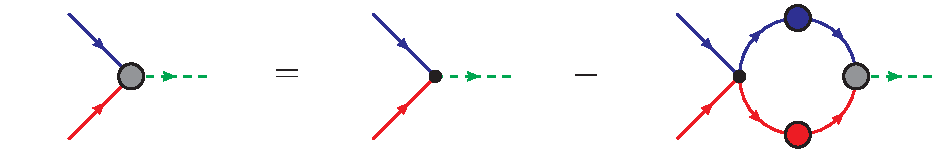
\includegraphics[width=0.7\textwidth]{figs/vertex3_DSE.pdf}\\
		\vspace{0.5cm}
		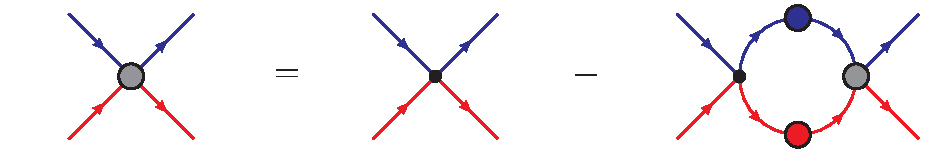
\includegraphics[width=0.7\textwidth]{figs/vertex4_DSE.pdf}
	\end{center}
	\caption[Vertex DSE]{Dyson-Schwinger equation for the three- and four-point function for the full Yukawa theory with background interactions, see~\cite{Diehl2006-1}.}
	\label{fig:vertex_prop_DSE}
\end{figure}


\clearpage

The other DSE's for the off-diagonal bosonic terms are, see Ref.~\cite{Fetter1971} on page 212,
\begin{align}
	\Gamma^{\phi^*\phi^*} &= S^{\psi_2\psi_1\phi^*}
	\frac{\delta}{\delta\Phi^*} G_{\psi_1\psi_2} = S^{\psi_2\psi_1\phi^*}
	\cdot G_{\psi_1\psi_2} \cdot \Gamma^{\psi_2\phi^*\psi_1} \cdot G_{\psi_1\psi_2} \notag \\
	&= h^2 \int_Q G_{\psi_1\psi_2}(Q)\cdot G_{\psi_1\psi_2}(P-Q) \,, \notag \\
	\Gamma^{\phi\phi} &= S^{\psi_2^*\psi_1^*\phi}
	\frac{\delta}{\delta\Phi} G_{\psi_1^*\psi_2^*} = S^{\psi_2^*\psi_1^*\phi}
	\cdot G_{\psi_1^*\psi_2^*} \cdot \Gamma^{\psi_2^*\phi\psi_1^*} \cdot G_{\psi_1^*\psi_2^*} \notag \\
	&= h^2 \int_Q G_{\psi_1^*\psi_2^*}(Q)\cdot G_{\psi_1^*\psi_2^*}(P-Q) \,.
\end{align}

Also in this case, we can see the symmetry $\Gamma^{\phi\phi}(P) = \Gamma^{\phi^*\phi^*}(-P)^*$.

In the end, we have a bosonic matrix with entries
\begin{align}
	\Gamma^{\Phi\Phi^{\dagger}} =
	\begin{pmatrix}
	\Gamma_{\phi}^{11} & \Gamma_{\phi}^{12} \\
	\Gamma_{\phi}^{21} & \Gamma_{\phi}^{22}
	\end{pmatrix} =
	\begin{pmatrix}
	\Gamma^{\phi\phi^*} & \Gamma^{\phi\phi} \\
	\Gamma^{\phi^*\phi^*} & \Gamma^{\phi^*\phi}
	\end{pmatrix} \,,
\end{align}
which satisfies
\begin{align}
	G_{\Phi\Phi^{\dagger}} = \left(\Gamma^{\Phi\Phi^{\dagger}}\right)^{-1} \,,
\end{align}
and has entries
\begin{align}
	G_{\Phi\Phi^{\dagger}} =
	\begin{pmatrix}
	G_{\phi\phi^*} & G_{\phi\phi} \\
	G_{\phi^*\phi^*} & G_{\phi^*\phi}
	\end{pmatrix}
	= \frac{1}{\Gamma_{\phi}^{11}\Gamma_{\phi}^{22}
	-\Gamma_{\phi}^{12}\Gamma_{\phi}^{21}}
	\begin{pmatrix}
	\Gamma_{\phi}^{22} & -\Gamma_{\phi}^{12} \\
	-\Gamma_{\phi}^{21} & \Gamma_{\phi}^{11}
	\end{pmatrix} \,.
\end{align}

For the normal boson propagator, e.g., we have~\cite{Perali2004}
\begin{align}
	G_{\phi\phi^*}(Q) = \frac{\chi_{11}(-Q)}{\chi_{11}(Q)\chi_{11}(-Q)-\chi_{12}(Q)^2} \,,
\end{align}
where $\chi_{11}(Q) = S^{\phi\phi^*}(Q) + \Pi_{11}(Q)$ and $\chi_{12}(Q) = \Pi_{12}(Q)$~\cite{Pieri2004-1}.


\clearpage

\section{Matsubara sums}
\label{app:matsubara-sums}

In this Appendix, we calculate the Matsubara sum in the fermion self-energy, see Eq.~\eqref{eq:spectral-sums},
\begin{align}
	I_{\psi}(\omega_n,\lambda_1,\lambda_2)
	= T \sum_{\Omega_m}
	\frac{1}{i\Omega_m-\lambda_1}
    \frac{1}{i(\Omega_m-\omega_n)-\lambda_2} \,,
\end{align}
where $\Omega_m=2m\pi T$ are bosonic frequencies and $\omega_n=(2n+1)\pi T$
are fermionic~\mbox{frequencies}.

The Bose-Einstein distribution $n_B(z)=1/(e^{\beta z}-1)$ has simple
poles at $z=i\Omega_n$ with residue $1/\beta$, and the Fermi distribution
$n_F(z)=1/(e^{\beta z}+1)$ has simple poles at $z=i\omega_n$ with residue
$-1/\beta$.

The integral along the contour $\mathcal{C}$ over bosonic/fermionic
frequencies $\omega_n$ gives~\cite{Punk2010}
\begin{align}
	T \sum_{\omega_n} h(i\omega_n) =
	\pm \oint_{\mathcal{C}} n_{B/F}(z) h(z) =
	\pm \sum_n
	\mathrm{Res}[n_{B/F}(z) h(z), i\omega_n] \,.
\end{align}
If the function $h(z)$ is analytical on the imaginary axis and vanishes
at infinity, one can deform the contour to exclude the poles on the
imaginary axis and pick up the poles $z_n$ of $h(z)$. Note that the contour
$\mathcal{C}'$ runs clockwise now.
\begin{align}
	T \sum_{\omega_n} h(i\omega_n) =
	\pm \oint_{\mathcal{C}'} n_{B/F}(z) h(z) =
	\mp \sum_n \mathrm{Res}[h(z), z_n] n_{B/F}(z_n) \,.
\end{align}

Applying this to our example above gives
\begin{align}
	I_{\psi}(\omega_n,\lambda_1,\lambda_2)
	&= \oint_{\mathcal{C}'} n_B(z)
	\frac{1}{z-\lambda_1}
    \frac{1}{z-i\omega_n-\lambda_2} \notag \\
    &= \frac{-n_B(\lambda_1)}{-i\omega_n+\lambda_1-\lambda_2} -
    \frac{n_B(i\omega_n+\lambda_2)}{i\omega_n-\lambda_1+\lambda_2} \notag \\
    &= \frac{-n_B(\lambda_1)-n_F(\lambda_2)}{-i\omega_n+\lambda_1-\lambda_2} \,,
\end{align}
where we used $n_B(i\omega_n+z)=-n_F(z)$ for fermionic frequencies in the last line~\cite{Punk2010}.

Analogously for the Matsubara sum in the boson self-energy, see Eq.~\eqref{eq:spectral-sums},
\begin{align}
	I_{\phi}(\omega_n,\lambda_1,\lambda_2)
	= T \sum_{\Omega_m}
	\frac{1}{i\Omega_m-\lambda_1}
    \frac{1}{i(\omega_n-\Omega_m)-\lambda_2} \,,
\end{align}
where now $\Omega_m=(2m+1)\pi T$ are fermionic frequencies and $\omega_n=2n\pi T$
are bosonic~\mbox{frequencies}.
\begin{align}
	I_{\phi}(\omega_n,\lambda_1,\lambda_2)
	&= -\oint_{\mathcal{C}'} n_F(z)
	\frac{1}{z-\lambda_1}
    \frac{1}{i\omega_n-z-\lambda_2} \notag \\
    &= \frac{n_F(\lambda_1)}{i\omega_n-\lambda_1-\lambda_2} -
    \frac{n_F(i\omega_n-\lambda_2)}{i\omega_n-\lambda_1-\lambda_2} \notag \\
    &= \frac{1-n_F(\lambda_1)-n_F(\lambda_2)}{-i\omega_n+\lambda_1+\lambda_2} \,,
\end{align}
where we now used $n_F(i\omega_n+z)=n_F(z)$ for bosonic frequencies. Additionally, we can use the important identities $n_F(-z)=1-n_F(z)$ and $n_B(-z)=-1-n_B(z)$.

\clearpage


\section{Renormalization}
\label{app:renormalization}

In this Appendix, we detail the renormalization procedure and the determination of the model parameters. For more details, see also~\cite{Diehl2006-1,Diehl2008,Punk2010,Schmidt2013}.

The assumption of a pure contact interaction in the single-channel model~\eqref{eq:single-channel-action} leads to unphysical divergences in the theory. In the real world, however, interactions always have a finite range $r_e$ and, thus, a natural momentum cutoff $\Lambda\sim 1/r_e$. In ultracold Fermi gases, the effective range is on the order of the van der Waals length $l_{\mathrm{vdw}}$~\cite{Schmidt2013}. On the other side, one finds that low-energy scattering physics is completely described by the scattering length $a$ and does not depend on the explicit form of the potential. Using this fact, one can regularize the theory and then take the limit of zero range interactions in the end.

We note that the momentum integral in the boson self-energy~\eqref{eq:self-energies} is linearly divergent and needs regularization. This is provided by the renormalization of $\nu$, which will cure all divergences of the theory. The physical renormalization condition is given by the connection to the two-body scattering length $a$ in vacuum~\cite{Schmidt2011,Frank2018-1}. The scattering of two fermions is mediated by the exchange of the bosonic dimer $\phi$. Evaluating the tree-level diagram for the effective fermion-fermion scattering in Fig.~\ref{fig:two-body-scattering} shows that the scattering amplitude $f(k)$ is related to the full boson propagator $G_{\phi}$ via~\cite{Schmidt2011,Zwerger2016}
%
\begin{align}
	\label{eq:scattering-amplitude-propagator}
	f(k) = \frac{h^2}{8\pi} G_{\phi}(2k^2,\bm{0}) \,,
\end{align}
%
where $E=2k^2$ is the total energy in the center of mass frame of incoming fermions with momenta $k$. This expression should be equal to the well-known result from low-energy s-wave scattering theory with zero effective range~\cite{Frank2018-1,Schmidt2013}
%
\begin{align}
	f(k) = \frac{1}{-1/a-ik} \,.
\end{align}
%
Thus, the renormalization condition for two-body scattering in vacuum is
%
\begin{align}
	G_{\phi}(0,\bm{0}) = -\frac{8\pi a}{h^2} \,.
\end{align}
%
This can be written in terms of the bare detuning $\nu$,
%
\begin{align}
	\nu = -\frac{h^2}{8\pi a} + \tilde{\Pi}_{\phi}(0,\bm{0}) \,,
\end{align}
%
where $\tilde{\Pi}_{\phi}$ is the bare boson self-energy. Thus, the renormalized boson DSE is
%
\begin{align}
	\Gamma^{(2)}_{\phi\phi^*}(\omega,\bm{p}) &= -\frac{h^2}{8\pi a} - \left[ \tilde{\Pi}_{\phi}(\omega,\bm{p}) - \tilde{\Pi}_{\phi}(0,\bm{0}) \right] \,.
\end{align}
%

\begin{figure}[h]
	\centering
	
\includegraphics[width=0.55\textwidth]{figs/two-body.pdf}
	\caption[Two-body scattering]{Tree-level diagram yielding the effective two-body scattering amplitude.}
	\label{fig:two-body-scattering}
\end{figure}

The renormalized boson self-energy $\Pi_{\phi}(\omega,\bm{p})=\tilde{\Pi}_{\phi}(\omega,\bm{p}) - \tilde{\Pi}_{\phi}(0,\bm{0})$, which also appears in Eq.~\eqref{eq:selfconsistent-equations}, is finite due to the counterterm $\tilde{\Pi}_{\phi}(0,\bm{0})$. To determine this counterterm, one has to consider the two-body problem in vacuum, i.e. $T=\mu=0$. In this case, the full boson self-energy can be solved exactly~\cite{Diehl2006-1,Schmidt2013}, since the fermions are not dressed. Evaluating the self-energy loop integral with the bare fermion propagators yields
%
\begin{align}
	\tilde{\Pi}_{\phi}(0,\bm{0}) &= h^2 \int_{\bm{q}}^{\Lambda} \frac{1}{2\varepsilon_{\bm{q}}} = \frac{h^2\Lambda}{4\pi^2} \,,
\end{align}
%
where $\Lambda$ is the aforementioned momentum cutoff that regularizes the integral. This counterterm cures all linear divergences arising from the contact interaction and allows to take the limit of $\Lambda$ to infinity in the end. For example, the renormalized boson self-energy in vacuum is then
%
\begin{align}
	\Pi_{\phi}(\omega, \bm{p}) &= h^2 \int_{\bm{q}}^{\Lambda} \left[\frac{1}{-\omega+\varepsilon_{\bm{q}}+\varepsilon_{\bm{p-q}}-i0^+} - \frac{1}{2\varepsilon_{\bm{q}}}\right] \notag \\
	&= \frac{h^2}{8\pi} \sqrt{-\frac{\omega}{2}+\frac{\bm{p}^2}{4}-i0^+}  \,,
\end{align}
%
with $\Lambda\rightarrow\infty$. For this reason, we can formally write the bare detuning $\nu$ as~\cite{Haussmann2009,Zwerger2016}
%
\begin{align}
	\label{eq:renorm-detuning}
	\nu = -\frac{h^2}{8\pi a} + \int_{\bm{q}} \frac{1}{2\varepsilon_{\bm{q}}} \,.
\end{align}



\clearpage

%%%%%%%%%%%%%%%%%%%%%%%%%%%%
\section{Boson self-energy calculation}
\label{app:boson-self-energy-calculation}

In this Appendix, we show the explicit computations and analytic results for the boson self-energy with general spin and mass-imbalance. Throughout this part, we use the same notation as introduced in Section~\ref{section:polaron-theoretical-description}. We start from the general expression for the non-selfconsistent boson self-energy with mass-imbalance $\alpha$,
\begin{align}
	\Pi_{\phi}(\omega_n, \bm{p}) =
	h^2 \int_{\bm{q}} \left[ T\sum_{\Omega_m}
	G^{(0)}_{\downarrow}(\Omega_m, \bm{q})
	G^{(0)}_{\uparrow}(\omega_n-\Omega_m, \bm{p-q}) - \frac{1+\alpha}{2\bm{q}^2} \right] \,.
\end{align}
Inserting the classical fermion spectral functions, we obtain the well-known result
\begin{align}
	\Pi_{\phi}(\omega_n, \bm{p}) &= h^2 \int_{\bm{q}} \left[ T\sum_{\Omega_m}
	\frac{1}{i\Omega_m-\varepsilon^{(I)}_{\bm{q}}+\mu_{\downarrow}}
	\frac{1}{i(\omega_n-\Omega_m)-\varepsilon_{\bm{p-q}}+\mu_{\uparrow}} - \frac{1+\alpha}{2\bm{q}^2} \right] \notag \\
	&= h^2 \int_{\bm{q}} \left[ \frac{1-n_F(\varepsilon^{(I)}_{\bm{q}}-\mu_{\downarrow}) -  n_F(\varepsilon_{\bm{p-q}}-\mu_{\uparrow})}{-i\omega_n+\varepsilon^{(I)}_{\bm{q}}+\varepsilon_{\bm{p-q}}-\mu_{\downarrow}-\mu_{\uparrow}} - \frac{1+\alpha}{2\bm{q}^2} \right] \,,
\end{align}
where $\varepsilon^{(I)}_{\bm{p}}=\bm{p}^2\,(1-\alpha)/(1+\alpha)$. From here, one can obtain the real and imaginary part of the retarded self-energy $\Pi_{\phi}^R(\omega,\bm{p})$ after analytic continuation $i\omega_n\rightarrow\omega+i0^+$. It is useful to separate the boson self-energy into a vacuum part and a temperature-dependent part, $\Pi^{R}_{\phi} = \Pi^{R,0}_{\phi} + \Pi^{R,T}_{\phi}$, where the vacuum part is given by
\begin{align}
	\Pi^{R,0}_{\phi}(\omega, \bm{p}) =
	h^2 \int_{\bm{q}} \left[ \frac{1}{-\omega+\varepsilon^{(I)}_{\bm{q}}+\varepsilon_{\bm{p-q}}-\mu_{\downarrow}-\mu_{\uparrow}-i0^+} - \frac{1+\alpha}{2\bm{q}^2} \right] \,,
\end{align}
Performing the variable shift $\bm{q} \rightarrow \bm{q} + (1+\alpha)\bm{p}/2$ makes the angle integration trivial and we obtain further for the vacuum part
\begin{align}
	\Pi^{R,0}_{\phi}(\omega, \bm{p}) =
	\frac{h^2(1+\alpha)}{4\pi^2} \int_0^{\infty} dq \left[\frac{q^2}{q^2-y-i0^+}-1\right]
	= \frac{h^2(1+\alpha)}{8\pi} \sqrt{-y-i0^+} \,,
\end{align}
where we have defined
\begin{align}
	y = \frac{(1+\alpha)}{2}
	\left[\omega-\frac{(1-\alpha)}{2}p^2
	+\mu_{\uparrow}+\mu_{\downarrow}\right] \,.
\end{align}

The temperature-dependent part can be divided into the $\downarrow$ and $\uparrow$ contribution and is obtained by the same means
\begin{align}
	\Pi^{R,T}_{\phi,\downarrow}(\omega, \bm{p}) = -
	\frac{h^2(1+\alpha)}{4\pi^2} \int_0^{\infty}
	\frac{\chi_{\downarrow}(q) \, q^2 \, dq}{q^2-y-i0^+} \,,
\end{align}
\begin{align}
	\Pi^{R,T}_{\phi,\uparrow}(\omega, \bm{p}) = -
	\frac{h^2(1+\alpha)}{4\pi^2} \int_0^{\infty}
	\frac{\chi_{\uparrow}(q) \, q^2 \, dq}{q^2-y-i0^+} \,,
\end{align}
where we have defined the two angle-integrated functions $\chi_{\downarrow}(q)$ and $\chi_{\uparrow}(q)$.

The angle-integrated functions at finite temperature are given by
\begin{align}
	\chi_{\downarrow}(q) &= \int_{-1}^1 \frac{dx}{2} \,
	n_F\left(\frac{(1-\alpha)}{(1+\alpha)}
	\left[\bm{q}+(1+\alpha)\bm{p}/2\right]^2
	-\mu_{\downarrow}\right) \notag \\
	&=
	\begin{cases}
		n_F\left(\frac{(1-\alpha)}{(1+\alpha)}
		q^2-\mu_{\downarrow}\right) & ,\, \bm{p} = \bm{0} \\
		\frac{T}{2(1-\alpha)pq} \ln\left( \frac{
			n_F\left(\mu_{\downarrow}-\frac{(1-\alpha)}{(1+\alpha)}
			\left[q+(1+\alpha)p/2\right]^2\right)}{
			n_F\left(\mu_{\downarrow}-\frac{(1-\alpha)}{(1+\alpha)}
			\left[q-(1+\alpha)p/2\right]^2\right)}
		\right) & ,\, \bm{p} \neq \bm{0}
	\end{cases} \,,
\end{align}
\begin{align}
	\chi_{\uparrow}(q) &= \int_{-1}^1 \frac{dx}{2} \,
	n_F\left(\left[\bm{q}-(1-\alpha)\bm{p}/2\right]^2
	-\mu_{\uparrow}\right) \notag \\
	&=
	\begin{cases}
		n_F\left(q^2-\mu_{\uparrow}\right) & ,\, \bm{p} = \bm{0} \\
		\frac{T}{2(1-\alpha)pq} \ln\left( \frac{
			n_F\left(\mu_{\uparrow}-\left[q+(1-\alpha)p/2\right]^2\right)}{
			n_F\left(\mu_{\uparrow}-\left[q-(1-\alpha)p/2\right]^2\right)}
		\right) & ,\, \bm{p} \neq \bm{0}
	\end{cases} \,.
\end{align}
Here, $x=\cos(\theta_{\bm{pq}})$ and $\theta_{\bm{pq}}$ is the angle between the vectors $\bm{p}$ and $\bm{q}$. Note that these functions leaves a non-zero contribution in the vacuum for $\mu_{\downarrow},\mu_{\uparrow}>0$. For completeness, we give the results in the limit $T\rightarrow 0$, obtained by $n_F(x)\rightarrow\theta(-x)$,
\begin{align}
	\chi_{\downarrow}(q) &= \int_{-1}^1 \frac{dx}{2} \,
	\theta\left(\mu_{\downarrow}-\frac{(1-\alpha)}{(1+\alpha)}
	\left[\bm{q}+(1+\alpha)\bm{p}/2\right]^2
	\right) \notag \\
	&=
	\begin{cases}
		\theta\left(\mu_{\downarrow}-\frac{(1-\alpha)}{(1+\alpha)}
		q^2 \right) & ,\, \bm{p} = \bm{0} \\
		\frac{\theta\left( \mu_{\downarrow}-
			Q_{-}^2 \right)}{2(1-\alpha)pq} \left[
		\mu_{\downarrow}-Q_{-}^2 -
		\left(\mu_{\downarrow}-Q_{+}^2\right)
		\theta\left( \mu_{\downarrow}-Q_{+}^2 \right)
		\right] & ,\, \bm{p} \neq \bm{0}
	\end{cases} \,,
\end{align}
where $Q_{\pm}^2 = \frac{(1-\alpha)}{(1+\alpha)}\left[q\pm(1+\alpha)p/2\right]^2$ and
\begin{align}
	\chi_{\uparrow}(q) &= \int_{-1}^1 \frac{dx}{2} \,
	\theta\left(\mu_{\uparrow}-\left[\bm{q}-(1-\alpha)\bm{p}/2\right]^2
	\right) \notag \\
	&=
	\begin{cases}
		\theta\left(\mu_{\uparrow}-q^2\right) & ,\, \bm{p} = \bm{0} \\
		\frac{\theta\left( \mu_{\uparrow}-
			q_{-}^2 \right)}{2(1-\alpha)pq} \left[
		\mu_{\uparrow}-q_{-}^2 -
		\left(\mu_{\uparrow}-q_{+}^2\right)
		\theta\left( \mu_{\uparrow}-q_{+}^2 \right)
		\right] & ,\, \bm{p} \neq \bm{0}
	\end{cases} \,,
\end{align}
where $q_{\pm}^2 = \left[q\pm(1-\alpha)p/2\right]^2$. These results coincide with~\cite{Hu2022}, and~\cite{Punk2010} for $\alpha=0$.


The real and imaginary part can be obtained analytically by using the formula
\begin{align}
	\frac{1}{x-i0^+} = P\frac{1}{x} + i\pi\delta(x) \,,
\end{align}
%
where $P$ denotes the principal value. There are the following two cases:

-- If $y<0$: The integrals for the real part are well-defined and $\mathrm{Im}\,\Pi_{\phi} = 0$!

-- If $y\geq 0$: The imaginary part is given analytically
\begin{align}
	\mathrm{Im}\,\Pi^{R,T}_{\phi}(\omega, \bm{p}) = -\frac{h^2(1+\alpha)}{4\pi^2}\, \pi
	\int_0^{\infty} \chi(q) q^2 \delta(q^2-y) \, dq
	= -\frac{h^2(1+\alpha)}{8\pi} \sqrt{y} \, \chi(\sqrt{y}) \,.
\end{align}

The real-part at finite temperature can then be obtained via Kramers-Kronig relation with a 1-dimensional numerical principal value integral.

For the real part, one can use the following formulas~\cite{Hu2022}.

-- If $y < 0$, then the integral for the real part is well-defined and we get
\begin{align}
	\text{Re}\, \Pi^{R,T}_{\phi}(\omega, \bm{p}) = -
	\frac{h^2(1+\alpha)}{4\pi^2} \int_0^{\infty}
	\frac{\chi(q) \, q^2 \, dq}{q^2+|y|} \,.
\end{align}

-- If $y\geq 0$, then one needs the principle value integral and obtains~\cite{Hu2022}
\begin{align}
	\text{Re}\, \Pi^{R,T}_{\phi}(\omega, \bm{p}) =-
	\frac{h^2(1+\alpha)}{4\pi^2}\, P\int_0^{\infty}
	\frac{\chi(q) \, q^2 \, dq}{q^2-y} 
	= -\frac{h^2(1+\alpha)}{8\pi^2} (C_1 + C_2)\,,
\end{align}
where
\begin{align}
	C_1 &= \int_y^{\infty}
	d\lambda\, \frac{\sqrt{y+\lambda}\chi(\sqrt{y+\lambda})}{\lambda} \,, \\
	C_2 &= \int_0^y
	d\lambda\, \frac{\sqrt{y+\lambda}\chi(\sqrt{y+\lambda})-\sqrt{y-\lambda}\chi(\sqrt{y-\lambda})}{\lambda} \,.
\end{align}

This formula can be derived from the following representation of the Kramers-Kronig relation, which is also useful for other numerical computations of the real part,
\begin{align}
	\text{Re}\,\Pi^R(\omega,\bm{p}) &= \int_{-\infty}^{\infty}\frac{d\lambda}{\pi}\, \frac{\text{Im}\,\Pi^R(\lambda,\bm{p})}{\lambda-\omega} \notag \\
	&= \int_{0}^{\infty}\frac{d\lambda}{\pi}\, \frac{\text{Im}\,\Pi^R(\omega+\lambda,\bm{p})-\text{Im}\,\Pi^R(\omega-\lambda,\bm{p})}{\lambda} \,.
\end{align}
This leads to the terms $C_1 + C_2$, if $y-\lambda\geq 0$, and to only $C_1$, if $y-\lambda<0$.

At $T=0$, the real part can be calculated analytically. For $\alpha=0$, our results coincide with~\cite{Punk2010}. Note that the following expressions are valid for positive chemical potential only, otherwise, they vanish.

First, we consider $\text{Re}\,\Pi^{R,T}_{\phi,\downarrow}$  ($\mu_{\downarrow} > 0$):
\begin{align}
	\text{Re}\, \Pi^{R,T}_{\phi,\downarrow}(\omega,\bm{0}) &= \frac{h^2(1+\alpha)}{4\pi^2} 
	\begin{cases}
		\sqrt{\frac{(1+\alpha)\mu_{\downarrow}}{(1-\alpha)}}-\sqrt{y}\,
		\text{arctanh}\left(\sqrt{\frac{(1+\alpha)\mu_{\downarrow}}{(1-\alpha)y}}\right) & ,\, y \geq 0 \\
		\sqrt{\frac{(1+\alpha)\mu_{\downarrow}}{(1-\alpha)}} - \sqrt{|y|} \arctan\left( \sqrt{\frac{(1+\alpha)\mu_{\downarrow}}{(1-\alpha)|y|}}\right) & ,\, y < 0
	\end{cases}	\,.
\end{align}


\begin{align}
	\text{Re}\, \Pi^{R,T}_{\phi,\downarrow}(\omega,\bm{p}) =\,
	&\frac{h^2(1+\alpha)}{8\pi^2} \left[
	\sqrt{\frac{(1+\alpha)\mu_{\downarrow}}{(1-\alpha)}} - \frac{y-\frac{(1+\alpha)\mu_{\downarrow}}{(1-\alpha)}+\frac{(1+\alpha)^2p^2}{4}}{2p(1+\alpha)}\log\left(\frac{y-\tilde{Q}^2_{+}}{y-\tilde{Q}^2_{-}}\right)\right. \notag \\
	&- \sqrt{|y|}\left.
	\begin{cases}
		\text{arctanh}\left(\frac{\tilde{Q}_{-}}{\sqrt{y}}\right) + 
		\text{arctanh}\left(\frac{\tilde{Q}_{+}}{\sqrt{y}}\right) & ,\, y \geq 0 \\
		\text{arctan}\left(\frac{\tilde{Q}_{-}}{\sqrt{|y|}}\right) + 
		\text{arctan}\left(\frac{\tilde{Q}_{+}}{\sqrt{|y|}}\right) & ,\, y < 0
	\end{cases}
	\right] \,,
\end{align}
with $\tilde{Q}_{\pm} = \sqrt{\frac{(1+\alpha)\mu_{\downarrow}}{(1-\alpha)}} \pm \frac{(1+\alpha)}{2}p$.

Finally, for $\text{Re}\,\Pi^{R,T}_{\phi,\uparrow}$ ($\mu_{\uparrow} > 0$):
\begin{align}
	\text{Re}\, \Pi^{R,T}_{\phi,\uparrow}(\omega,\bm{0}) &= \frac{h^2(1+\alpha)}{4\pi^2} 
	\begin{cases}
		\sqrt{\mu_{\uparrow}}-\sqrt{y}\,
		\text{arctanh}\left(\sqrt{\frac{\mu_{\uparrow}}{y}}\right) & ,\, y \geq 0 \\
		\sqrt{\mu_{\uparrow}} - \sqrt{|y|} \arctan\left( \sqrt{\frac{\mu_{\uparrow}}{|y|}}\right) & ,\, y < 0
	\end{cases}	\,.
\end{align}

\begin{align}
	\text{Re}\, \Pi^{R,T}_{\phi,\uparrow}(\omega,\bm{p}) =\,
	&\frac{h^2(1+\alpha)}{8\pi^2} \left[
	\sqrt{\mu_{\uparrow}} - \frac{y-\mu_{\uparrow}+\frac{(1-\alpha)^2p^2}{4}}{2p(1-\alpha)}\log\left(\frac{y-\tilde{q}^2_{+}}{y-\tilde{q}^2_{-}}\right)\right. \notag \\
	&- \sqrt{|y|}\left.
	\begin{cases}
		\text{arctanh}\left(\frac{\tilde{q}_{-}}{\sqrt{y}}\right) + 
		\text{arctanh}\left(\frac{\tilde{q}_{+}}{\sqrt{y}}\right) & ,\, y \geq 0 \\
		\text{arctan}\left(\frac{\tilde{q}_{-}}{\sqrt{y}}\right) + 
		\text{arctan}\left(\frac{\tilde{q}_{+}}{\sqrt{y}}\right) & ,\, y < 0
	\end{cases}
	\right] \,,
\end{align}
with $\tilde{q}_{\pm} = \sqrt{\mu_{\uparrow}} \pm \frac{(1-\alpha)}{2}p$. \\

Fig.~\ref{fig:boson-self-energy} shows an example for the real and imaginary part of the retarded boson self-energy $\Pi^{R}_{\phi}(\omega,\bm{p})$ for the balanced case at unitarity and $\beta\mu=0.13146$.\footnote{Note the confusion with the signs for the boson self-energy as compared to the literature \ 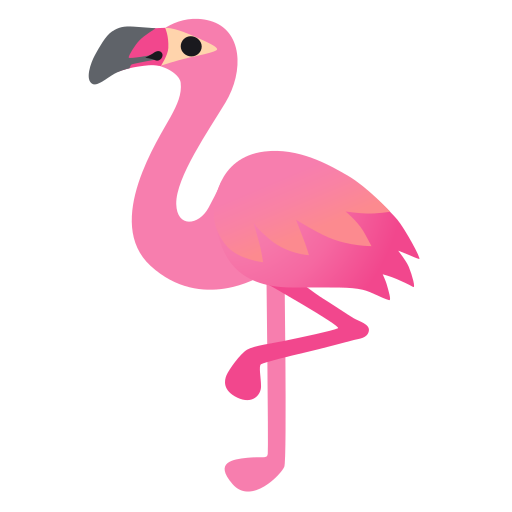
\includegraphics[width=0.025\textwidth]{figs/flamingo.png}}

\vspace{1cm}

\begin{figure*}[h]
	\centering
	\subfigure[$\text{Re}\,\Pi^{R}_{\phi}(\omega,\bm{p})$]{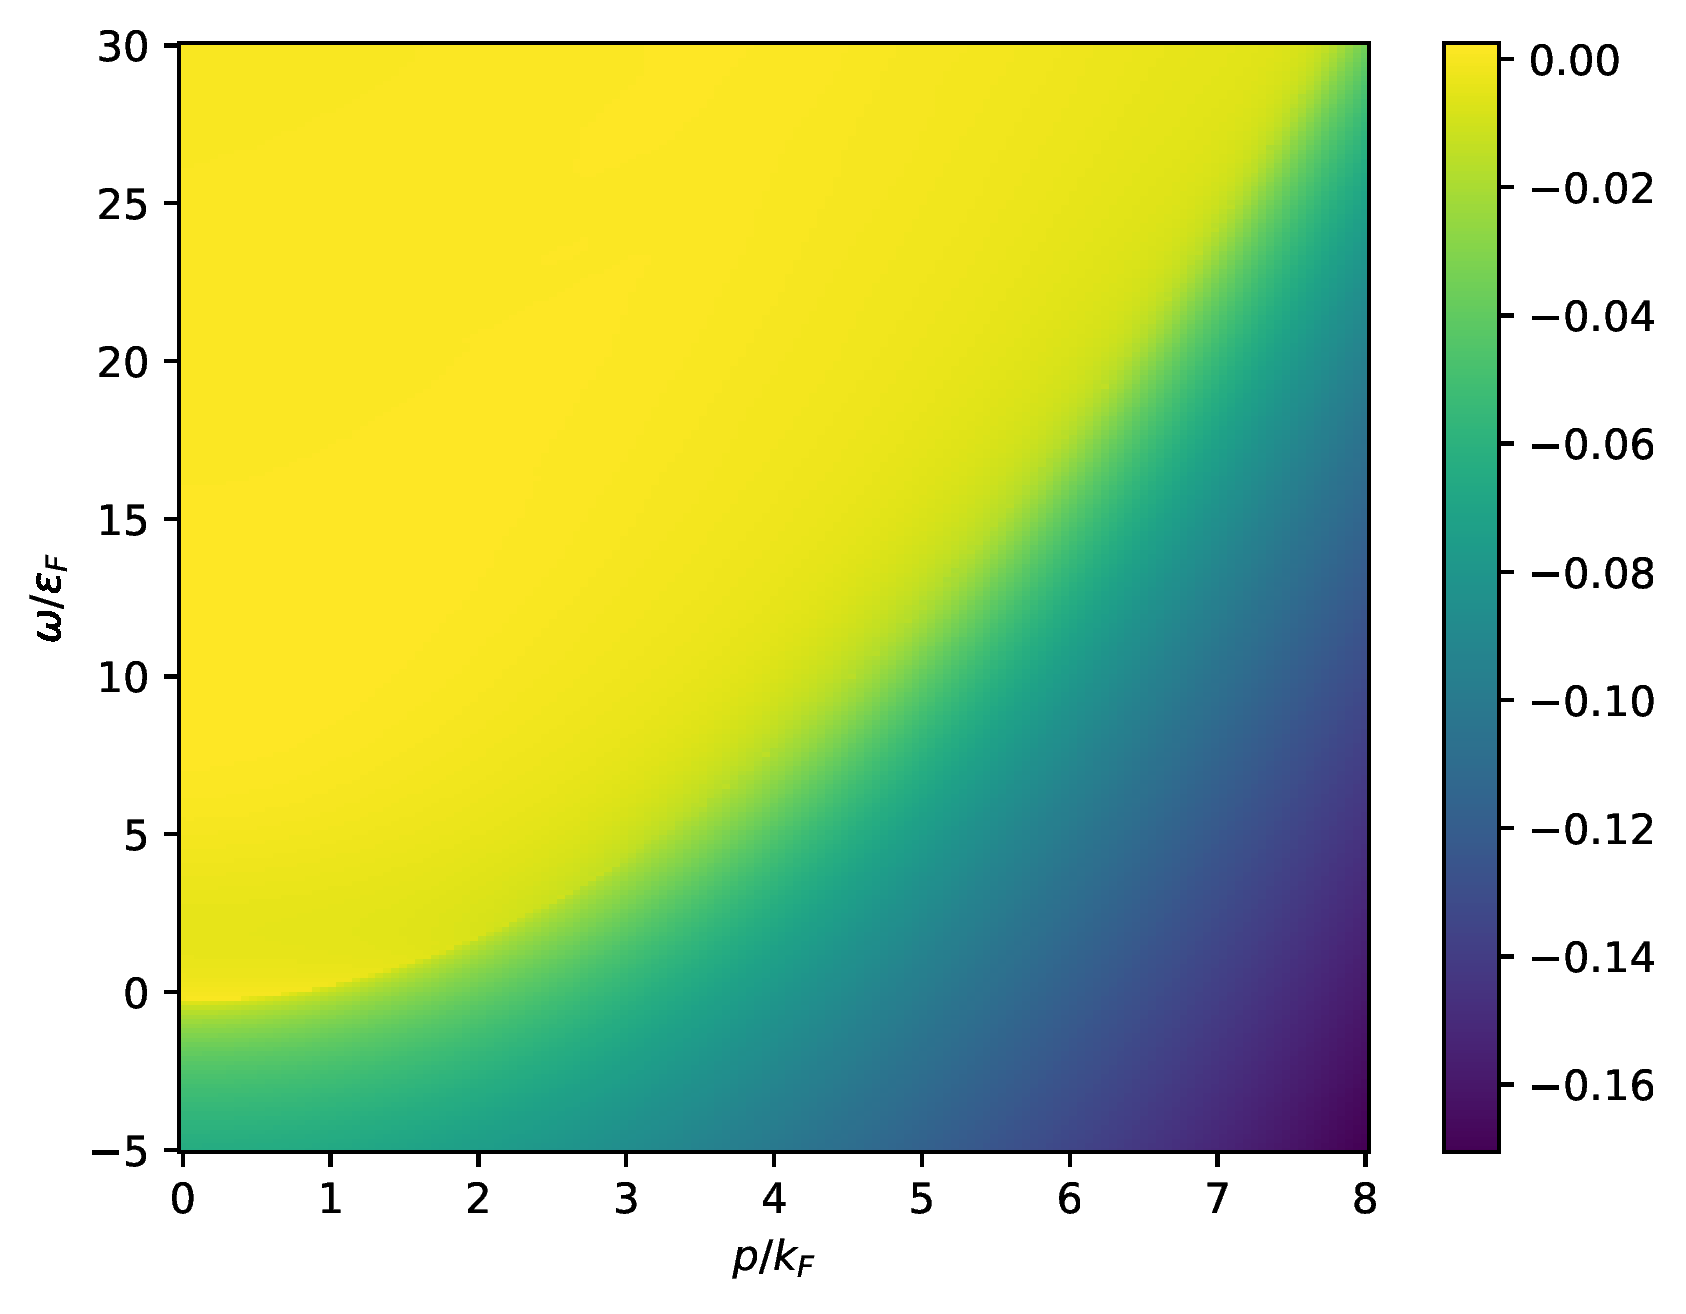
\includegraphics[width=0.475\textwidth]{figs/boson_self_re.png}}
	\subfigure[$\text{Im}\,\Pi^{R}_{\phi}(\omega,\bm{p})$]{\includegraphics[width=0.47\textwidth]{figs/boson_self_im.png}}
	\caption[Boson self-energy]{Real and imaginary part of the retarded boson self-energy $\Pi^{R}_{\phi}(\omega,\bm{p})$.}
	\label{fig:boson-self-energy}
\end{figure*}


\clearpage

%%%%%%%%%%%%%%%%%%%%%%%%%%%%
\section{Fermion self-energy calculation}
\label{app:fermion-self-energy-calculation}


For the fermion self-energy, there are no analytical results for the non-selfconsistent case in the single-channel model, since the bare boson propagator has no dispersion. Therefore, the self-energy has to be computed numerically from the spectral functions. The general expression for the retarded fermion self-energy $\Sigma^R_{\psi}(\omega,\bm{p})$ is
%
\begin{align}
	\label{eq:ferm_self}
	\Sigma^R_{\psi}(\omega,\bm{p}) = -h^2\int_{\bm{q},\lambda_1,\lambda_2} \rho_{\phi}(\lambda_1,\bm{q}) \rho_{\psi}(\lambda_2,\bm{p}-\bm{q})\, \frac{n_B(\lambda_1)+n_F(\lambda_2)}{-\omega+\lambda_1-\lambda_2-i0^+} \,,
\end{align}
%
Taking the imaginary part recovers Eq.~\eqref{eq:imaginary-part-self-energies}. Note that the imaginary part is strictly negative, since all quantities are positive definite, except of $n_B(\lambda_1)$ and $\rho_{\phi}(\lambda_1)$. Fortunately, the sign change of the boson distribution and spectral function occurs both at $\lambda_1=0$, and $n_B(\lambda_1),\rho_{\phi}(\lambda_1)<0$ for $\lambda_1<0$. Moreover, the pole of $n_B(\lambda_1)$ at $\lambda_1=0$ is exactly canceled by the zero crossing of the boson spectral function $\rho_{\phi}(\lambda_1)$, see Section~\ref{section:spectral-representation}. Thus, the imaginary part of Eq.~\eqref{eq:ferm_self} is a regular expression that can be evaluated numerically. The only difficulty is the highly peaked structure of the integrand, and will be discussed in the numerical Appendix~\ref{app:numerical-implementation}.

As a side remark, we note that non-selfconsistent results for the fermion self-energy can be derived for the two-channel model with dynamic bosons. Inserting the classical spectral functions $\rho_{\psi}(\lambda,\bm{p})=\delta(\lambda-\bm{p}^2+\mu)$ and $\rho_{\phi}(\lambda,\bm{p})=\delta(\lambda-\bm{p}^2/2-\nu+2\mu)$, we obtain
\begin{align}
\Sigma^R_{\psi}(\omega, \bm{p}) = -h^2 \int_{\bm{q}} \frac{n_B(\varepsilon_{\bm{q}}/2+\nu-2\mu) + n_F(\varepsilon_{\bm{p-q}}-\mu)}{-\omega+\varepsilon_{\bm{q}}/2- \varepsilon_{\bm{p-q}}+\nu-\mu-i0^+} \,.
\end{align}
However, this will not be evaluated further in this work. \\

Fig.~\ref{fig:fermion-self-energy} shows an example for the real and imaginary part of the retarded fermion self-energy $\Sigma^{R}_{\psi}(\omega,\bm{p})$ for the balanced case at unitarity and $\beta\mu=0.13146$.

\vspace{1cm}

\begin{figure*}[h]
	\centering
	\subfigure[$\text{Re}\,\Sigma^{R}_{\psi}(\omega,\bm{p})$]{\includegraphics[width=0.47\textwidth]{figs/fermion_self_re.png}}
	\subfigure[$\text{Im}\,\Sigma^{R}_{\psi}(\omega,\bm{p})$]{\includegraphics[width=0.47\textwidth]{figs/fermion_self_im.png}}
	\caption[Fermion self-energy]{Real and imaginary part of the retarded fermion self-energy $\Sigma^{R}_{\psi}(\omega,\bm{p})$.}
	\label{fig:fermion-self-energy}
\end{figure*}
	\chapter{Numerical Implementation}
\label{app:numerical-implementation}

The numerical implementation of the self-consistent equations was performed mainly
in \verb|Python 3.9| and partially in \verb|Mathematica|. Some of the numerical methods are inspired by the work of J. Winkel in our group, see~\cite{Winkel2021} for more details. The main steps and ideas of the present numerical framework are:

\begin{enumerate}
\item First iteration of the boson propagator: \\
Start with the analytic expression for $\text{Im}\,\Pi^R_{\phi}$ and calculate $\text{Re}\,\Pi^R_{\phi}$ on a finite grid. To simplify the calculation, treat the divergent vacuum part analytically, see below. \\
Choose grid size large enough such that the numerical corrections are quite small. This can be quantified in dependence of the temperature.
\item First iteration of the fermion propagator: \\
Take the bare fermion spectral function (delta peak) and the semi-analytic boson spectral function from the first iteration and calculate $\text{Im}\,\Sigma^R_{\psi}$ with~\eqref{eq:imaginary-part-self-energies} on a finite grid. From this, obtain $\text{Re}\,\Sigma^R_{\psi}$ as described below.
\item Further iterations of the fermion propagator: \\
Take the numerical spectral functions for the fermion and boson and calculate the self-energy as in step 2.
\item Further iterations of the boson propagator: \\
Take numerical spectral functions for the fermions and calculate $\text{Im}\,\Pi^R_{\phi}$ on a finite grid. Outside the grid, glue smoothly to the analytical non-selfconsistent result. Compute the difference $\delta\text{Re}\,\Pi^R_{\phi}$ to the non-selfconsistent result.
\end{enumerate}

For the numerical calculation of 2-dimensional functions an adaptive python package, called \verb|Adaptive|~\cite{Nijholt2019}, is used. The sampling points are chosen automatically based on the functional form. Less samples are taken in smoother regions and more samples are taken in faster changing regions. Additionally, the calculation of these sampling points can be parallelized over multiple cores. An example of how sampling points are taken by \verb|Adaptive| is shown in Fig.~\ref{fig:adaptive}. The resulting sampling points are then linearly interpolated. It is useful to simplify the interpolation by deforming the functions onto the quadratic dispersion relation, see Fig.~\ref{fig:shift_dispersion}. For the bosonic self-energy, this step can significantly improve the resolution of sharp edges in the function. For the fermionic self-energy, it can additionally help to ensure a large enough distance of the grid boundary to the main peak, such that asymptotic behavior is visible. 

The numerical integration of the self-energy loop integrals is performed mainly with an adaptive Monte Carlo method from \verb|Vegas+|~\cite{Lepage2021}. This allows for maximal flexibility when dealing with highly peaked integrands in a multidimensional space and can be generalized easily. However, this comes with the downside of a long runtime. For this specific use case, a different adaptive integration routine using sparse grids might be more efficient. The 1-dimensional principal value integral for the real part of the self-energy is computed using the adaptive quadrature integration from \verb|SciPy|~\cite{Virtanen2019}.

\begin{figure}[h]
	\centering
	\includegraphics[width=0.58\textwidth]{figs/adaptive.png}
	\caption[Evaluation of a function with Adaptive]{Example of a 2-dimensional function evaluated by Adaptive.}
	\label{fig:adaptive}
\end{figure}

\begin{figure}[h]
	\centering
	\subfigure[]{\includegraphics[width=0.46\textwidth]{figs/dispersion-shift1.png}} 
	\subfigure[]{\includegraphics[width=0.46\textwidth]{figs/dispersion-shift2.png}}
	\caption[Improving sampling and interpolation of 2d functions with sharp edges]{Procedure to improve the interpolation of sharp edges and curvy functions. (a) A 2-dimensional function is transformed onto the dispersion relation and linearly interpolated $f(\omega,\bm{p})$. (b) Afterwards, the interpolated function is shifted back to the dispersion relation $f(\omega-\bm{p}^2/2,\bm{p})$.}
	\label{fig:shift_dispersion}
\end{figure}


%%%%%%%%%%%%%%%%%%%%%%%%%%%%
\subsection*{Boson spectral function}
\label{subsec:boson_spec}

In this Section, we detail the calculation and representation of the boson spectral function $\rho_{\phi}$. Since the renormalized bosonic self-energy~\eqref{eq:self-energies} includes a counterterm, the numerical procedure requires suitable subtraction schemes and analytic treatment. 

The problematic part is the well-known vacuum solution, which is given by
%
\begin{align}
\Pi^0_{\phi}(\omega_n, \bm{p}) &= h^2 \int_{\bm{q}} \left[\frac{1}{-i\omega_m+\varepsilon_{\bm{q}}+\varepsilon_{\bm{p-q}}-2\mu} - \frac{1}{2\varepsilon_{\bm{q}}}\right] \notag \\
&= \frac{h^2}{8\pi} \sqrt{-\frac{i\omega_n}{2}+\frac{\bm{p}^2}{4}-\mu}  \,.
\end{align}
%
This means that the vacuum part,
%
\begin{align}
\mathrm{Im}\,\Pi^{R,0}_{\phi}(\omega, \bm{p}) = \frac{h^2}{8\pi} \sqrt{\frac{\omega}{2}-\frac{\bm{p}^2}{4}+\mu}  \,,
\end{align}
%
can be subtracted from the total numerical self-energy $\mathrm{Im}\,\Pi^{R}_{\phi}(\omega, \bm{p})$ in order to treat the divergent real part analytically. Thus, we calculate the full numerical imaginary part of the self-energy and obtain the real part via
%
\begin{align}
\mathrm{Re}\,\Pi^{R}_{\phi}(\omega, \bm{p}) &= \mathrm{Re}\,\Pi^{R,0}_{\phi}(\omega, \bm{p}) \notag \\
&+ \frac{1}{\pi} \int_{\lambda} \frac{\mathrm{Im}\,\Pi^R_{\phi}(\lambda,\bm{p})-\mathrm{Im}\,\Pi^{R,0}_{\phi}(\lambda,\bm{p})}{\lambda-\omega} \,,
\end{align}
%
where $\mathrm{Re}\,\Pi^{R,0}_{\phi}(\omega, \bm{p})$ is the real part of the vacuum solution
%
\begin{align}
\mathrm{Re}\,\Pi^{R,0}_{\phi}(\omega, \bm{p}) = -\frac{h^2}{8\pi} \sqrt{-\frac{\omega}{2}+\frac{\bm{p}^2}{4}-\mu} \,.
\end{align}
%
With these formulas, we can obtain $\mathrm{Im}\,\Pi^{R}_{\phi}$ and $\mathrm{Re}\,\Pi^{R}_{\phi}$ on a finite grid numerically.

However, the calculation of the real part requires also information about the high frequency tails outside the numerical grid. In this case, the imaginary part outside the grid is approximated by the analytic formula of the non-selfconsistent self-energy discussed in the previous Section,
%
\begin{align}
\mathrm{Im}\,\Pi^{R}_{\phi}(\omega, \bm{p})-\mathrm{Im}\,\Pi^{R,0}_{\phi}(\omega, \bm{p}) \approx \mathrm{Im}\,\Pi^{R,T}_{\phi}(\omega, \bm{p}) \,,
\end{align}
%
for large $\omega$. Thus, the bosonic spectral function outside the grid is approximated by the non-selfconsistent spectral function $\rho^{(1)}_{\phi}$ (first iteration). A different subtraction scheme would be to subtract the whole non-selfconsistent imaginary part straightaway and only deal with differences to the first iteration. In principle, both methods are equivalent and work similar. For practical reasons, we choose the latter subtraction scheme.

Another trick to improve the numerical calculation was already mentioned above. Since the boson self-energy follows a quadratic dispersion relation, it is practical to transform the functions onto the dispersion relation before interpolation, as shown in Fig.~\ref{fig:shift_dispersion}. This way, a better sampling and interpolation of the important regions can be achieved. Afterwards, the interpolated function is shifted back to the correct dispersion relation.

Since the fermion spectral functions in the self-energy integrals are very peaked for lower temperatures and larger momenta, it might be useful to subtract a broadened classical spectral function, or the first iteration, from the further iterations in order to improve the integration for larger momenta. The contribution from the subtracted spectral function has then to be taken into account. Since the fermion spectral functions are represented on a finite numerical grid, the bare delta peak contributions from outside the grid has to be taken into account too. This is similar to the peak-tail splits from~\cite{Horak2019}.

For the representation of the numerical self-energy on the finite grid, an adaptive grid is chosen for the imaginary and real part, separately. The boundaries in frequency are $\omega=(-100,100)\,\varepsilon_F$ and in momentum $p=(0,10)\,k_F$. Approximately 10.000 grid points are needed to obtain stable numerical results.


%%%%%%%%%%%%%%%%%%%%%%%%%%%%
\subsection*{Calculation of the real part via Kramers-Kronig}
\label{subsec:real-part}

It turns out that the calculation of the real part via Kramers-Kronig relation is very sensitive to the high frequency tails of the imaginary part. It is not sufficient to know the imaginary part on a finite grid, but rather, we have to extrapolate the high frequency behavior and estimate its contribution. For constant momentum $p$, the large-frequency behavior of the self-energy $\mathrm{Im}\,\tilde{\Sigma}^{R}(\omega)$ outside the numerical grid is well described by the power law
%
\begin{align}
\mathrm{Im}\,\tilde{\Sigma}^{R}(\omega) \approx \frac{a}{\omega^b} \,,
\end{align}
%
where the constants $a,b$ are determined by a fitting routine. From this fit one can calculate the missing contribution $\delta\mathrm{Re}\,\tilde{\Sigma}^{R}(\omega)$ for the real part at frequency $\omega$. We express the imaginary part as $\mathrm{Im}\,\tilde{\Sigma}^{R}(\lambda) = \mathrm{Im}\,\Sigma^{R}(\lambda)\theta(\omega_{\mathrm{max}}-\lambda) + a\lambda^{-b} \theta(\lambda-\omega_{\mathrm{max}})$ with a contribution inside and outside the numerical grid with frequency cutoff $\omega_{\mathrm{max}}$. From the Kramers-Kronig relation, we obtain the contribution outside the grid
%
\begin{align}
	\delta\mathrm{Re}\,\tilde{\Sigma}^{R}(\omega) = \int_{\Delta}^{\infty}\frac{\mathrm{Im}\,\tilde{\Sigma}^{R}(\omega+\lambda)\,d\lambda}{\pi\lambda} = \int_{\Delta}^{\infty}\frac{a\,d\lambda}{\pi\lambda(\omega+\lambda)^b} \,,
\end{align}
%
where $\Delta=\omega_{\mathrm{max}}-\omega$. Evaluating the last integral gives the analytic expression
%
\begin{align}
\delta\mathrm{Re}\,\tilde{\Sigma}^{R}(\omega) = \frac{a}{\pi\Delta^b b}\,{}_{2}F_{1}\left(b,b;1+b;-\frac{\omega}{\Delta}\right) \,,
\end{align}
%
where ${}_{2}F_{1}\left(a,b;c;z\right)$ is the hypergeometric function~\cite{Abramowitz1972}. Using this large-frequency contribution from outside the grid, improves the determination of the real part significantly. For the fermion self-energy, we observe $b\approx 0.5$ for large enough $\omega_{\mathrm{max}}$.

This asymptotic behavior can be shown by similar arguments as in Ref.~\cite{Schneider2009}. We consider only the large frequency behavior and rewrite the imaginary part of the fermion self-energy in~\eqref{eq:imaginary-part-self-energies} as
%
\begin{align}
	\mathrm{Im}\,\Sigma^R_{\psi}(\omega) \sim \int_{\bm{q},\lambda_1,\lambda_2}
	\rho_{\phi}(\lambda_1) \rho_{\psi}(\lambda_2)
	\delta(\omega-\lambda_1+\lambda_2) \left[n_B(\lambda_1)+n_F(\lambda_2)\right] \,.
\end{align}
%
In the limit $\omega\rightarrow\infty$, the delta function only contributes if (a) $\lambda_1$ large and $\lambda_2$ small or (b) $\lambda_2$ large negative and $\lambda_1$ small. In case (b), however, the fermion spectral function $\rho_{\psi}$ vanishes for small momenta and $\lambda_2\rightarrow-\infty$. Thus, only case (a) contributes and we are left with
%
\begin{align}
\mathrm{Im}\,\Sigma^R_{\psi}(\omega) \sim \int_{\bm{q},\lambda_2} \rho_{\phi}(\omega+\lambda_2) \rho_{\psi}(\lambda_2) n_F(\lambda_2) \,,
\end{align}
%
where we have used $n_B(\lambda_1)\rightarrow 0$ for $\lambda_1\rightarrow\infty$. As seen above, the large frequency behavior of the boson spectral function is dominated by $\rho_{\phi}(\omega)\sim 1/\sqrt{\omega}$. Additionally, the integrand vanishes for large negative values of $\lambda_2$, since $\rho_{\psi}(\lambda_2)$ vanishes, and for large positive values of $\lambda_2$, since $n_F(\lambda_2)$ vanishes. Thus, the range of $\lambda_2$ is limited and we can write
%
\begin{align}
\mathrm{Im}\,\Sigma^R_{\psi}(\omega) \sim \int_{\bm{q},\lambda_2} \rho_{\psi}(\lambda_2) n_F(\lambda_2) / \sqrt{\omega} \sim 1/\sqrt{\omega} \,,
\end{align}
%
where we used that $\int_{\bm{q},\lambda_2} \rho_{\psi}(\lambda_2) n_F(\lambda_2) = n$ is finite in the last step.


With the same argument one can show that $\mathrm{Im}\,\Sigma^R_{\psi}(\omega)$ vanishes rapidly for large negative frequency. 



%%%%%%%%%%%%%%%%%%%%%%%%%%%%
\subsection*{Iterative procedure}
\label{subsec:iteration}

Using~\eqref{eq:imaginary-part-self-energies} and the Kramers-Kronig relation, the retarded self energies can be computed in every iteration step and fed back into the next, after extraction of the spectral function via~\eqref{eq:spectral-relation}. The iterative procedure is initialized with the classical fermion spectral function,
%
\begin{align} \label{eq:inital-fermion-spec}
\rho^{(0)}_{\psi}(\omega,\bm{p}) = \delta(\omega-\bm{p}^2+\mu) \,.
\end{align}
%
This initial guess is inserted into the spectral form of $\Pi_{\phi}$ to obtain the first iteration of the boson spectral function $\rho_{\phi}^{(1)}$. Then, $\rho_{\phi}^{(1)}$ together with $\rho^{(0)}_{\psi}$ are inserted into the spectral integral of $\Sigma_{\psi}$ to obtain the first iteration of the fermion spectral function $\rho_{\psi}^{(1)}$. Now, $\rho_{\psi}^{(1)}$ can be used to obtain the next iteration for the boson spectral function $\rho_{\phi}^{(2)}$, and so on. In general, $\rho_{\psi}^{(i)}$ is used to obtain $\rho_{\phi}^{(i+1)}$, and $\rho_{\phi}^{(i+1)}$ and $\rho_{\psi}^{(i)}$ are used to obtain $\rho_{\psi}^{(i+1)}$. This iteration is repeated until convergence is reached. We observe that around 5-20 iterations are needed to obtain a converged result with ($\Lambda$: numerical momentum cutoff)
%
\begin{align}
\int_{\bm{q},\lambda}^{\Lambda} \left| \rho^{(i)}(\lambda,\bm{q})-\rho^{(i-1)}(\lambda,\bm{q}) \right| \lesssim 0.005\, \Lambda \,.
\end{align}
%
This criterion is similar to the statement that, at this point, the density $n^{(i)}$ obtained from the $i$th iteration does not change significantly anymore. In our case, the accuracy is around $1\%$.
As mentioned in the main text, the convergence is worse closer to the critical temperature and the spectral functions may jump around. One can improve the convergence by iterating twice over the fermions or updating the spectral functions only partially. Other methods are discussed in the main text.
}

\cleardoublepage
\pagenumbering{Roman}
%References, Figures etc.
\thispagestyle{plain}
\addcontentsline{toc}{chapter}{References}
\nocite{*}
\printbibliography[title=References]
\cleardoublepage

{\hypersetup{linkcolor=black}
\listoffigures
\addcontentsline{toc}{chapter}{List of Figures}
}	
\cleardoublepage
\thispagestyle{plain}
\section*{Acknowledgements}
First of all, I would like to thank Jan M. Pawlowski for providing me with the opportunity to work on such exciting and challenging topic during which I learned a lot.

Secondly, I thank Richard Schmidt for many discussions and for being the second referee of this thesis.

Furthermore, I thank Jan Horak, Friederike Ihssen and Jonas Wessely for many discussions and constant emotional support during good and bad times, and also for proofreading and comments on this thesis.

I would also like to thank my office mates Gioele Casagranda, Marcel Horstmann and Anton Kreuzkamp for discussions and making the time more enjoyable. I thank Gioele Casagranda for proofreading and comments on this work.

I thank Jonas von Milczewski, Marcel Gievers and Xin Chen for helpful discussions.

I thank Felipe Attanasio and Marc Bauer for discussions and providing their lattice data for comparion. Moreover, I thank Bernhard Frank, Martin W. Zwierlein and Biswaroop Mukherjee for providing their data.

Finally, a big thanks goes to Johannes Lang for many helpful discussions, during which I learned a lot, and also for taking the time to compare results.




\section*{Declaration of Authorship}
I hereby certify that this thesis has been composed by me and is based on my own work, unless stated otherwise.\\

Heidelberg, 08.08.2023 \hfill \rule{50mm}{.15mm} \par

\end{document}